\documentclass[12pt]{report}
\usepackage{graphicx}     %Note graphics<graphicx<epsfig
\usepackage[table,xcdraw, dvipsnames]{xcolor}
\usepackage{hyperref} %written by Sebastian Rahtz
%\usepackage{subeqn}    %allows equations 1a, 1b
%\usepackage{subfig}    %allows figures 1a, 1b
\usepackage{amsmath}
\usepackage{amssymb}
\usepackage{xurl}
\usepackage{bbm}%for indicator function
%\bibliographystyle{alpha}
\usepackage{floatrow}
\usepackage[normalem]{ulem}


\usepackage{tocloft}

% Adjust number widths
\setlength{\cftchapnumwidth}{2em}
\setlength{\cftsecnumwidth}{3.2em}
\setlength{\cftsubsecnumwidth}{3.5em}

\usepackage[toc,page]{appendix}
\usepackage[nottoc]{tocbibind}

\usepackage[color,matrix,frame,arrow,curve]{xy}
\usepackage[shortlabels]{enumitem}
\usepackage{array}
\usepackage{pdflscape}
\usepackage{multicol, multirow}
\usepackage{ctable}
\usepackage{dirtree}
\usepackage{subfig}
\usepackage{longtable}

%\usepackage{fdsymbol}
%\usepackage{animate}% play animation

\usepackage[vlined,ruled]{algorithm2e}
\newcommand{\mycommfont}[1]{\small\ttfamily\textcolor{blue}{#1}}
\SetCommentSty{mycommfont}

%highlighting
\usepackage{mdframed}

\usepackage[makeroom]{cancel}

\usepackage{pdfpages}
\usepackage{hyperxmp}

% this escapes the underscore in text
%\usepackage[T1]{fontenc}
%\usepackage{underscore}

\paperheight=11in
\topmargin=0in
\headheight=0in
\headsep=0in
\topskip=0in
\textheight=8.5in
\footskip=.5in


\paperwidth=8.5in
\oddsidemargin=.25in
\evensidemargin=.25in
\textwidth=6.0in
\parindent=.5in

\newcommand{\chapquote}[3]{\begin{quotation} \textit{#1} \end{quotation} \begin{flushright} - #2, \textit{#3}\end{flushright} }

\newtheorem{claim}{Claim}
\newcommand{\proof}[0]{{\bf proof:} }
\newcommand{\qed}[0]{\quad\newline \noindent{\bf QED }}

\newcommand{\upto}[0]{-}
\newcommand{\XT}[2]{{\substack{#1\\#2}}}

\newcommand{\bra}[1]{\langle#1|}
\newcommand{\ket}[1]{|#1\rangle}
\newcommand{\av}[1]{\left\langle#1\right\rangle}
\newcommand{\pder}[2]{\frac{\partial#1}{\partial#2}}
\newcommand{\der}[2]{\frac{d#1}{d#2}}
\newcommand{\tr}[0]{{\rm tr }}
\newcommand{\beq}{\begin{equation}}
\newcommand{\eeq}{\end{equation}}
\newcommand{\bsub}{\begin{subequations}}
	\newcommand{\esub}{\end{subequations}}
\newcommand{\beqa}{\begin{eqnarray}}
\newcommand{\eeqa}{\end{eqnarray}}
\newcommand{\rarrow}[0]{\rightarrow}
\newcommand{\larrow}[0]{\leftarrow}
\newcommand{\uarrow}[0]{\uparrow}
\newcommand{\darrow}[0]{\downarrow}
\newcommand{\Rarrow}[0]{\Rightarrow}
\newcommand{\nRarrow}[0]{\nRightarrow}
\newcommand{\Larrow}[0]{\Leftarrow}
\newcommand{\nLarrow}[0]{\nLeftarrow}
\newcommand{\ul}[1]{\uline{#1}}
\newcommand{\ol}[1]{\overline{#1}}
\newcommand{\CC}[0]{{ \mathbb{C}} }
\newcommand{\EE}[0]{{ \mathbb{E}} }
\newcommand{\NNN}[0]{ {\mathbb{N}}} %\NN already defined
\newcommand{\RR}[0]{{ \mathbb{R}} }
\newcommand{\WW}[0]{ {\mathbb{W}}}
\newcommand{\XX}[0]{{ \mathbb{X}} }
\newcommand{\ZZ}[0]{ {\mathbb{Z}}}

\newcommand{\ground}{{}_{\stackrel{\stackrel{\displaystyle{\bot}}{-}}{.}}}
\newcommand{\norm}[1]{\parallel#1\parallel}
\newcommand{\eqdef}[0]{\;\;\stackrel{\text{def}}{=}\;\;}

\newcommand{\heavy}[0]{\mathbf{H}}

\newcommand{\rva}[0]{{\ul{a}}}
\newcommand{\rvb}[0]{{\ul{b}}}
\newcommand{\rvc}[0]{{\ul{c}}}
\newcommand{\rvd}[0]{{\ul{d}}}
\newcommand{\rve}[0]{{\ul{e}}}
\newcommand{\rvf}[0]{{\ul{f}}}
\newcommand{\rvg}[0]{{\ul{g}}}
\newcommand{\rvh}[0]{{\ul{h}}}
\newcommand{\rvi}[0]{{\ul{i}}}
\newcommand{\rvj}[0]{{\ul{j}}}
\newcommand{\rvk}[0]{{\ul{k}}}
\newcommand{\rvl}[0]{{\ul{l}}}
\newcommand{\rvll}[0]{{\ul{\ell}}}
\newcommand{\rvm}[0]{{\ul{m}}}
\newcommand{\rvn}[0]{{\ul{n}}}
\newcommand{\rvo}[0]{{\ul{o}}}
\newcommand{\rvp}[0]{{\ul{p}}}
\newcommand{\rvq}[0]{{\ul{q}}}
\newcommand{\rvr}[0]{{\ul{r}}}
\newcommand{\rvs}[0]{{\ul{s}}}
\newcommand{\rvt}[0]{{\ul{t}}}
\newcommand{\rvu}[0]{{\ul{u}}}
\newcommand{\rvv}[0]{{\ul{v}}}
\newcommand{\rvw}[0]{{\ul{w}}}
\newcommand{\rvx}[0]{{\ul{x}}}
\newcommand{\rvy}[0]{{\ul{y}}}
\newcommand{\rvz}[0]{{\ul{z}}}


\newcommand{\rvA}[0]{{\ul{A}}}
\newcommand{\rvB}[0]{{\ul{B}}}
\newcommand{\rvC}[0]{{\ul{C}}}
\newcommand{\rvD}[0]{{\ul{D}}}
\newcommand{\rvE}[0]{{\ul{E}}}
\newcommand{\rvF}[0]{{\ul{F}}}
\newcommand{\rvG}[0]{{\ul{G}}}
\newcommand{\rvH}[0]{{\ul{H}}}
\newcommand{\rvI}[0]{{\ul{I}}}
\newcommand{\rvJ}[0]{{\ul{J}}}
\newcommand{\rvK}[0]{{\ul{K}}}
\newcommand{\rvL}[0]{{\ul{L}}}
\newcommand{\rvM}[0]{{\ul{M}}}
\newcommand{\rvN}[0]{{\ul{N}}}
\newcommand{\rvO}[0]{{\ul{O}}}
\newcommand{\rvP}[0]{{\ul{P}}}
\newcommand{\rvQ}[0]{{\ul{Q}}}
\newcommand{\rvR}[0]{{\ul{R}}}
\newcommand{\rvS}[0]{{\ul{S}}}
\newcommand{\rvT}[0]{{\ul{T}}}
\newcommand{\rvU}[0]{{\ul{U}}}
\newcommand{\rvV}[0]{{\ul{V}}}
\newcommand{\rvW}[0]{{\ul{W}}}
\newcommand{\rvX}[0]{{\ul{X}}}
\newcommand{\rvY}[0]{{\ul{Y}}}
\newcommand{\rvZ}[0]{{\ul{Z}}}

\newcommand{\rvbeta}[0]{{\ul{\beta}}}
\newcommand{\rvxi}[0]{{\ul{\xi}}}
\newcommand{\rvzeta}[0]{{\ul{\zeta}}}
\newcommand{\rvtheta}[0]{{\ul{\theta}}}
\newcommand{\rvmu}[0]{{\ul{\mu}}}
\newcommand{\rvsig}[0]{{\ul{\sigma}}}
\newcommand{\rvDel}[0]{{\ul{\Delta}}}
\newcommand{\rvtau}[0]{{\ul{\tau}}}

\newcommand{\cala}[0]{{\cal A}}
\newcommand{\calb}[0]{{\cal B}}
\newcommand{\calc}[0]{{\cal C}}
\newcommand{\cald}[0]{{\cal D}}
\newcommand{\cale}[0]{{\cal E}}
\newcommand{\calf}[0]{{\cal F}}
\newcommand{\calg}[0]{{\cal G}}
\newcommand{\calh}[0]{{\cal H}}
\newcommand{\cali}[0]{{\cal I}}
\newcommand{\calk}[0]{{\cal K}}
\newcommand{\call}[0]{{\cal L}}
\newcommand{\calm}[0]{{\cal M}}
\newcommand{\caln}[0]{{\cal N}}
\newcommand{\calo}[0]{{\cal O}}
\newcommand{\calp}[0]{{\cal P}}
\newcommand{\calq}[0]{{\cal Q}}
\newcommand{\calr}[0]{{\cal R}}
\newcommand{\cals}[0]{{\cal S}}
\newcommand{\calt}[0]{{\cal T}}
\newcommand{\calu}[0]{{\cal U}}
\newcommand{\calv}[0]{{\cal V}}
\newcommand{\calw}[0]{{\cal W}}
\newcommand{\calx}[0]{{\cal X}}
\newcommand{\caly}[0]{{\cal Y}}
\newcommand{\calz}[0]{{\cal Z}}

%\newcommand{\diamante}[1]{\Big\langle#1\Big\rangle}
\newcommand{\diamante}[1]{*++[F=]{#1}}
%\newcommand{\corchete}[1]{\Big\{#1\Big\}}
\newcommand{\corchete}[1]{#1}
\newcommand{\cuadro}[1]{*++[F]{#1}}

\newcommand{\Pmat}[4]{\calp\left[
\begin{array}{cc}#1&#2\\#3&#4
\end{array}\right]}

%\newcommand{\PN}[0]{PN^{0,0}_{1,1}}
%\newcommand{\PS}[0]{PS^{1,1}_{0,0}}
\newcommand{\PN}[0]{PN}
\newcommand{\PS}[0]{PS}

\newcommand{\lam}[0]{\lambda}
\newcommand{\Lam}[0]{\Lambda}
\newcommand{\alp}[0]{\alpha}
\newcommand{\eps}[0]{\epsilon}
\newcommand{\s}[0]{\sigma}
\newcommand{\su}[0]{{\Sigma}}

\newcommand{\pp}[0]{\mathbb{P}}
\newcommand{\dbm}[0]{{
		[1,\partial_{b},\partial_{m}]
}}

\newcommand{\dg}[0]{{[1, \partial_{\theta_G}]}}
\newcommand{\dd}[0]{{[1, \partial_{\theta_D}]}}
\newcommand{\dgd}[0]{{[1, \partial_{\theta_G}, \partial_{\theta_D}]}}

\newcommand{\veca}[0]{{\vec{a}}}
\newcommand{\vecb}[0]{{\vec{b}}}
\newcommand{\vecc}[0]{{\vec{c}}}
\newcommand{\vecd}[0]{{\vec{d}}}
\newcommand{\vecf}[0]{{\vec{f}}}
\newcommand{\vech}[0]{{\vec{h}}}
\newcommand{\vecr}[0]{{\vec{r}}}
\newcommand{\vecs}[0]{{\vec{s}}}
\newcommand{\vecu}[0]{{\vec{u}}}
\newcommand{\vecx}[0]{{\vec{x}}}
\newcommand{\vecy}[0]{{\vec{y}}}
\newcommand{\vechy}[0]{{\vec{\haty}}}
\newcommand{\vtheta}[0]{{\vec{\theta}}}

\newcommand{\haty}[0]{{\widehat{y}}}
\newcommand{\hatx}[0]{{\widehat{x}}}
\newcommand{\hata}[0]{{\widehat{a}}}
\newcommand{\hatr}[0]{{\widehat{r}}}


\newcommand{\cond}[0]{{\:\mathbf{|}\:}}
\newcommand{\mymathbf}[1]{#1}

\newcommand{\ranvec}[1]{\ul{\vec{#1}}}
\newcommand{\indi}[0]{\mathbbm{1}}
\newcommand{\smoid}[0]{{\rm smoid}}
\newcommand{\lodds}[0]{{\rm lodds}}
\newcommand{\expit}[0]{{\rm expit}}
\newcommand{\logit}[0]{{\rm logit}}
\newcommand{\sign}[0]{{\rm sign}}

\renewcommand{\labelitemii}{$\bullet$}

\newcommand{\HAT}[1]{{\widehat{#1}}}
\newcommand{\TIL}[1]{{\widetilde{#1}}}
\newcommand{\tild}[0]{{\TIL{d}}}
\newcommand{\tile}[0]{{\TIL{e}}}
\newcommand{\tilg}[0]{{\TIL{g}}}
\newcommand{\tilu}[0]{{\TIL{u}}}
\newcommand{\tilx}[0]{{\TIL{x}}}
\newcommand{\tilP}[0]{{\TIL{P}}}
\newcommand{\tilPT}[0]{{\TIL{P}_\theta}}

\newcommand{\maparrow}[1]
{\xymatrix{\ar[r]_{#1}&}}


\newcommand{\ucalm}[0]{\ul{\calm}}

\newcommand{\bool}[0]{\{0,1\}}

\newcommand{\argmin}{\mathop{\mathrm{argmin}}\limits}
\newcommand{\argmax}{\mathop{\mathrm{argmax}}\limits}

\newcommand{\softmax}[0]{{\rm softmax}}

\newcommand{\A}[0]{\wedge}
\newcommand{\V}[0]{\vee}
\newcommand{\xor}{\oplus}
\newcommand{\bigA}[0]{\bigwedge}
\newcommand{\bigV}[0]{\bigvee}
\newcommand{\bigxor}{\bigoplus}


\newcommand{\rdart}[0]{\Rightarrow}
\newcommand{\ldart}[0]{\Leftarrow}
\newcommand{\rveps}[0]{\ul{\eps}}

\newcommand{\hatvar}[0]{\widehat{\sigma^2}}
\newcommand{\ptp}[0]{{(t)}}

\newcommand{\tseries}[1]{{\{#1\}_{\forall t}}}

\newcommand{\xbeta}[0]{X_\s^T\beta}
\newcommand{\xtau}[0]{X_\s^T\tau}

%arguments phi1, phi2, phi3, e
\newcommand{\rbd}[4]{
\xymatrix@-1.3pc{
&#1\ar[d]&&#2\ar[d]
\\
&\rvx_1\ar[rr]
&&
\rvx_2
\ar `r[rd][rd]
\\
0\ar`u[u][ru]
\ar`d[dr][rrd]
&&&&\rvA\ar[r]&#4
\\
&&
\rvx_3
\ar `r[rru][rru]
\\
&&#3\ar[u]
}
}

\newcommand{\rulezeroif}[0]{
If $(\rvb. \perp \rva.
|\rvr., \rvs.)$
in $G$, then}

\newcommand{\rulezerothen}[0]{
$\rva.=a. \leftrightarrow 1$}

\newcommand{\rulezeroP}[0]{
P(b.|a.,r.,s.)=P(b.|r., s.)}

\newcommand{\rulezeroH}[0]{
H(\rvb.:\rva.|\rvr.,\rvs.)=0}

\newcommand{\rulezeropic}[0]{
\xymatrix@C=1pc@R=1pc{
&r.\ar[dr]
&s.\ar[d]
\\
a.\ar[rr]
&&b.
&=
}
\xymatrix@C=1pc@R=1pc{
&r.\ar[dr]&s.\ar[d]
\\
a.\ar[rr]|0
&&b.
}}

\newcommand{\ruleoneif}[0]{
If $(\rvb. \perp \rva.
|\rvr., \rvs.)$
in $\cald_{\rvr.} G$, then}

\newcommand{\ruleonethen}[0]{
$\rva.=a. \leftrightarrow 1$}

\newcommand{\ruleoneP}[0]{
P(b.|a., \cald\rvr.=r.,s.)=
P(b.|\cald\rvr.=r., s.)}

\newcommand{\ruleoneH}[0]{
H(\rvb.:\rva.|\cald\rvr.,\rvs.)=0}

\newcommand{\ruleonepic}[0]{
\xymatrix@C=1pc@R=1pc{
&\cald\rvr.=r.\ar[dr]
&s.\ar[d]
\\
a.\ar[rr]
&&b.
&=
}
\xymatrix@C=1pc@R=1pc{
&\cald\rvr.=r.\ar[dr]
&s.\ar[d]
\\
a.\ar[rr]|0
&&b.
}}

\newcommand{\ruletwoif}[0]{
If $(\rvb.\perp \rva. |
 \rvr., \rvs.)$
in $\call_{\rva.}\cald_{\rvr.} G$,
 then}

\newcommand{\ruletwothen}[0]{
$\cald \rva.=a. \leftrightarrow \rva.=a.$}

\newcommand{\ruletwoP}[0]{
P(b.|\cald\rva.=a., \cald\rvr.=r., s.)=
P(b.|a., \cald\rvr.=r.,  s.)}

\newcommand{\ruletwoH}[0]{
H(\rvb.:\cald\rva.|\cald\rvr.,  \rvs.)
=
H(\rvb.:\rva.|\cald\rvr.,  \rvs.)}

\newcommand{\ruletwopicA}[0]{
\xymatrix@C=1pc@R=1pc{
\;\ar[d]_0
&\cald\rvr.=r.\ar[dr]
&s.\ar[d]
\\
\cald\rva.=a.\ar[rr]\ar[d]
&&b.
&=\quad\quad
\\
&
}
\xymatrix@C=1pc@R=1pc{
\;\ar[d]_0
&&\cald\rvr.=r.\ar[dr]
&s.\ar[d]
\\
\cald\rva.=a.\ar[d]
&a.\ar[rr]
&&b.
\\
&
}}
\newcommand{\ruletwopicB}[0]{
\xymatrix@C=1pc@R=1pc{
\;\ar[d]
&\cald\rvr.=r.\ar[dr]
&s.\ar[d]
\\
a.\ar[rr]\ar[d]
&&b.
&=\quad\quad
\\
&
}
\xymatrix@C=1pc@R=1pc{
\;\ar[d]
&&\cald\rvr.=r.\ar[dr]
&s.\ar[d]
\\
a.\ar[d]
&\cald\rva.=a.\ar[rr]
&&b.
\\
&
}}

\newcommand{\rulethreeif}[0]{
If $
(\rvb. \perp \rva.
| \rvr., \rvs.)$
in $\cald_{\rva.-an(\rvs.)}
\cald_{\rvr.}G$,
 then}

\newcommand{\rulethreethen}[0]{
$\cald \rva.=a. \leftrightarrow 1$}

\newcommand{\rulethreeP}[0]{
P(b.|\cald\rva.=a.,\cald\rvr.=r.,  s.)=
P(b.|\cald\rvr.=r., s.)}

\newcommand{\rulethreeH}[0]{
H(\rvb.:\cald\rva.|\cald\rvr., \rvs.)=0}

\newcommand{\rulethreepic}[0]{
\xymatrix@C=1pc@R=1pc{
&
&\cald\rvr.=r.\ar[dr]
&s.\ar[d]
\\
&\cald\rva.=a.\ar[rr]
&&b.
&=
}
\xymatrix@C=1pc@R=1pc{
&
&\cald\rvr.=r.\ar[dr]
&s.\ar[d]
\\
&\cald\rva.=a.\ar[rr]|0
&&b.
}}

\newcommand{\bdoordef}[0]{
Suppose that we have access to data
that allows us to
estimate a probability
distribution
 $P(x., y., z.)$.
Hence, the variables
$\rvx., \rvy., \rvz.$ are
ALL observed (i.e, not hidden).
Then we say that the
backdoor $\rvz.$
satisfies the
{\bf backdoor adjustment criterion}
relative to $(\rvx., \rvy.)$
if
\begin{enumerate}
\item
All backdoor paths from $\rvx.$
to $\rvy.$
 are blocked by  conditioning on
 $\rvz.$.
\item
$\rvz. \cap de(\rvx.)=\emptyset$.
\end{enumerate}
}

\newcommand{\bdoorclaim}[0]{
If $\rvz.$ satisfies the
backdoor criterion relative to
 $(\rvx., \rvy.)$, then

\beqa
P(y. | \cald \rvx.=x.)&=&
\sum_{z.} P(y.|x., z.)P(z.)
\\
&=&
\begin{array}{l}
\\
\\
\end{array}
\xymatrix{
\sum z.\ar[dr]
\\
x.\ar[r]
&y.
}
\eeqa
where $\sum z.$ means node
$\rvz.$ is summed over.
}

\newcommand{\fdoordef}[0]{
Suppose that we have access to data
that allows us to
estimate a probability
distribution
 $P(x., m., y.)$.
Hence, the variables
$\rvx., \rvm., \rvy.$ are
ALL observed (i.e, not hidden).
Then we say that
the frontdoor $\rvm.$
satisfies the
{\bf frontdoor adjustment criterion}
relative to $(\rvx., \rvy.)$
if
\begin{enumerate}
\item
All directed paths from
$\rvx.$ to $\rvy.$ are intercepted by
(i.e., have a node in) $\rvm.$.
\item
All backdoor paths from $\rvx.$ to
$\rvm.$ are blocked.
\item
All backdoor paths from
on $\rvm.$ to $\rvy.$
are blocked by conditioning
on  $\rvx.$.
\end{enumerate}
}

\newcommand{\fdoorclaim}[0]{
If $\rvm.$ satisfies the
frontdoor criterion
relative to $(\rvx., \rvy.)$,
and $P(x.,m.)>0$, then

\beqa
P(y. | \cald \rvx.=x.)&=&\sum_{m.}
\underbrace{\left[\sum_{x'.}
P(y.|x'., m.)P(x'.)\right]}_
{P(y.|\cald \rvm.=m.)}
\underbrace{P(m.|x.)}_
{P(m.|\cald \rvx.=x.)}
\\
&=&
\xymatrix{
&\sum x'.\ar[dr]
\\
x.´\ar[r]
&\sum m.\ar[r]&y.
}
\eeqa
where $\sum x'.$ and
$\sum m.$
means nodes
$\rvx'.$ and $\rvm.$
are summed over.
}


%Symmetry
\newcommand{\symrule}[0]{
$\rva\perp_P\rvb\implies \rvb\perp_P\rva$}

\newcommand{\symruleH}[0]{
$H(\rva:\rvb)=0\implies H(\rvb:\rva)=0$}

%Decomposition
\newcommand{\decrule}[0]{
$\rva\perp_P\rvb, \rvc\implies
\rva\perp_P\rvb \text{ and } \rva\perp_P\rvc$}

\newcommand{\decruleH}[0]{
$H(\rva:\rvb, \rvc)=0\implies
H(\rva:\rvb)=0 \text{ and } H(\rva:\rvc)=0$}

%Weak Union
\newcommand{\wearule}[0]{
$\rva\perp_P \rvb, \rvc \implies
\rva\perp_P\rvb|\rvc\text{ and }\rva\perp_P\rvc|\rvb$}

\newcommand{\wearuleH}[0]{
$H(\rva:\rvb, \rvc)=0 \implies
H(\rva:\rvb|\rvc)=0\text{ and }H(\rva:\rvc|\rvb)=0$}

%Contraction
\newcommand{\conrule}[0]{
$\rva\perp_P\rvb|\rvc\text{ and }\rva\perp_P \rvc
\implies \rva\perp_P \rvb, \rvc$}

\newcommand{\conruleH}[0]{
$H(\rva:\rvb|\rvc)=0\text{ and }H(\rva:\rvc)=0
\implies H(\rva:\rvb, \rvc)=0$}

%Intersection
\newcommand{\intrule}[0]{
$\rva\perp_P\rvb|\rvc, \rvd\text{ and }
\rva\perp_P \rvd|\rvc, \rvb\implies
\rva\perp_P \rvb,\rvd|\rvc$}

\newcommand{\intruleH}[0]{
$H(\rva:\rvb|\rvc, \rvd)=0\text{ and }
H(\rva:\rvd|\rvc, \rvb)=0\implies
H(\rva:\rvb,\rvd|\rvc)=0$}

\newcommand{\dotbarmu}[0]{{\cdot|\mu}}
\newcommand{\dotmu}[0]{{\cdot, \mu}}
\newcommand{\kbarmu}[0]{{k|\mu}}
\newcommand{\kmu}[0]{{k,\mu}}
\newcommand{\plusbarmu}[0]{{+|\mu}}
\newcommand{\plusmu}[0]{{+,\mu}}

\newcommand{\bnlearn}[0]{{\tt bnlearn\;}}

\newcommand{\sqsig}[0]{{[\sigma]}}

\newcommand{\misscellone}[0]{
\begin{array}{c}
\frac{1}{nsam}
P(x_0=0, x_2=0\cond x_1=1, \theta)
\\
\frac{1}{nsam}
P(x_0=0, x_2=1\cond x_1=1, \theta)
\\
\frac{1}{nsam}
P(x_0=1, x_2=0\cond x_1=1, \theta)
\\
\frac{1}{nsam}
P(x_0=1, x_2=1\cond x_1=1, \theta)
\end{array}
}

\newcommand{\misscelltwo}[0]{
\begin{array}{c}
\frac{1}{nsam}
P(x_1=0\cond x_0=0,x_2=1, \theta)
\\
\frac{1}{nsam}
P(x_1=1\cond x_0=0,x_2=1,  \theta)
\end{array}
}


\newcommand{\td}[0]{{\TIL{d}}}
\newcommand{\rvtd}[0]{{\ul{\TIL{d}}}}
\newcommand{\tx}[0]{{\TIL{x}}}
\newcommand{\tmu}[0]{{\TIL{\mu}}}
\newcommand{\rvtx}[0]{{\ul{\TIL{x}}}}

\newcommand{\mlarr}[0]{\xrightarrow{\rm ML-fit}}
\newcommand{\lrarr}[0]{\xrightarrow{\rm LR-fit}}

\newcommand{\setprob}[3]
{{\begin{array}{c}S=\{#1\}
\\P(S)=#2\\ \haty(x^\s_S)=\$#3 K
\end{array}}}

\newcommand{\Gno}[0]{\xymatrix{\;\ar[r]|\parallel_G&}}
\newcommand{\Gyes}[0]{\xymatrix{\;\ar[r]_G&}}

\newcommand{\calypso}[0]{\ol{\caly}}

\newcommand{\SeqBdoorDef}[0]{
Suppose that we have access to data
that allows us to
estimate a probability
distribution
 $P(x^n, y, z^n)$.
Hence, the variables
$\rvx^n, \rvy, \rvz^n$ are
ALL observed (i.e, not hidden).
Then we say that the
the multinode
of \enquote{covariates} $\rvz^n$
satisfies the
{\bf sequential backdoor (SBD) adjustment criterion}
relative to $(\rvx^n, \rvy)$
if for all $t\in\{0,1, \ldots, n-1\}$,

\begin{enumerate}
\item
$\rvy\perp\rvx_t|
\underbrace{(\rvx_0, \rvx_1, \ldots,\rvx_{t-1},
\rvz_0, \rvz_1, \ldots, \rvz_t)}
_{\text{Past of $\rvx_t$}}$
in $\call_{\rvx_{t}}
\cald_{\rvx_{t+1},\rvx_{t+2}
,\ldots, \rvx_{n-1}}G$.
\item
$\rvz_t \cap de(\rvx_t)=\emptyset$.
\end{enumerate}
}

\newcommand{\SeqBdoorClaim}[0]{
If $\rvz^n$ satisfies the
sequential backdoor criterion relative to
 $(\rvx^n, \rvy)$, then

\beq
P(y | \cald \rvx^n=x^n)=
\calq(y|x^n)
\;,
\eeq
where $\calq(y|x^n)$
is defined by
Eq.(\ref{def-q-y-xn-seqbdoor}).
}


\usepackage[T1]{fontenc}
\usepackage[english]{babel}
\usepackage{lmodern}
\usepackage[utf8]{inputenc}
\usepackage{csquotes}
\usepackage{listings}
\usepackage{xcolor}

\definecolor{codegreen}{rgb}{0,0.6,0}
\definecolor{codegray}{rgb}{0.5,0.5,0.5}
\definecolor{codepurple}{rgb}{0.58,0,0.82}
\definecolor{backcolour}{rgb}{0.95,0.95,0.92}

\lstdefinestyle{mystyle}{
    backgroundcolor=\color{backcolour},
    commentstyle=\color{codegreen},
    keywordstyle=\color{magenta},
    numberstyle=\tiny\color{codegray},
    stringstyle=\color{codepurple},
    basicstyle=\footnotesize,
    breakatwhitespace=false,
    breaklines=true,
    captionpos=b,
    keepspaces=true,
    numbers=left,
    numbersep=5pt,
    showspaces=false,
    showstringspaces=false,
    showtabs=false,
    tabsize=2
}
\lstset{style=mystyle}

% special commands of Shannon Info paper
\newcommand{\rv}[1]{{\,\ul{#1}\,}}
\newcommand{\tcall}[0]{{ \cal\widetilde{L} } }

\newcommand{\ptype}[1]{{P_{[#1]} } }
\newcommand{\ptiltype}[1]{{\widetilde{P}_{[#1]} } }

\newcommand{\sts}[1]{{S_{#1}}}
\newcommand{\zn}[0]{{Z_{1,N}}}
\newcommand{\rvxdot}[0]{{\ul{x_.}}}

\newcommand{\what}[1]{{\widehat{#1}}}
%\includeonly{conventions/conventions,rnn/rnn}


\begin{document}
\title{\textbf{Bayesuvius},
 \\a small visual dictionary of
 Bayesian Networks}



\author{Robert R. Tucci\\
        www.ar-tiste.xyz}

\date{ \today}

\maketitle

\begin{figure}[h!]
\centering
\includegraphics[width=5in]{vesuvius-from-pompei.png}
\caption{View of Mount Vesuvius from  Pompeii} 
\end{figure}

\begin{figure}[h!]
\centering
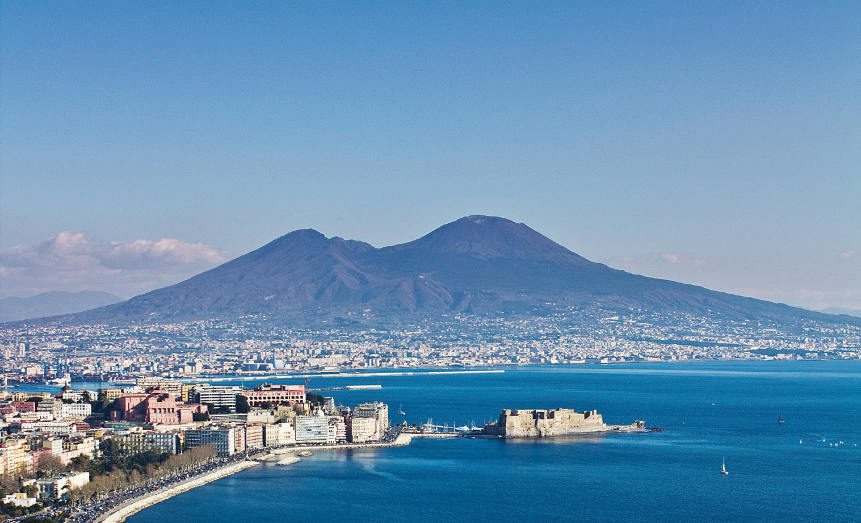
\includegraphics[width=5in]{vesuvius-bay-of-naples.jpg}
\caption{Mount Vesuvius and Bay of Naples} 
\end{figure}


\newpage
\tableofcontents
\section{Foreword}
Welcome to Bayesuvius! a proto-book uploaded to github.

A different Bayesian network is discussed
 in each chapter. Each chapter title is 
the name of a B net. Chapter titles are
 in alphabetical order.

This is a volcano in its early stages.
 First version uploaded to a github repo 
called Bayesuvius on June 24, 2020. 
First version only covers 2 B nets 
(Linear Regression and GAN). 
I will add more chapters periodically.
 Remember, this is a moonlighting effort 
so I can't do it all at once.

For any questions about notation, 
please go to Notational Conventions section.

Requests and advice are welcomed.


\bigskip
\noindent Thanks for reading this.

\noindent Robert R. Tucci

\noindent www.ar-tiste.xyz




\chapter*{Notational Conventions and Preliminaries}
\addcontentsline{toc}{chapter}{Notational Conventions and Preliminaries}

\label{ch0-conventions}
\section{Some abbreviations frequently
used throughout this book}

\begin{itemize}
\item
bnet= Bnet= Bayesian Network
\item
CPT = Conditional Probabilities Table,
 same as TPM
\item
DAG = Directed Acyclic Graph
\item
i.i.d.= independent identically
distributed.
 \item
 RCT= Randomized Controlled Trial,
a.k.a. A/B testing.

\item
TPM= Transition Probability Matrix,
same as CPT

\end{itemize}

\section{${\cal N}(!a)$}
$\caln(!a)$ will denote
a normalization constant that does not depend
on $a$. For example, $P(x)=\caln(!x)e^{-x}$
where $\int_0^\infty dx \;P(x)=1$.

\section{One hot vector}
A {\bf one hot  vector}
is a vector with all entries
equal to zero with
the exception of a single entry which is one.
A {\bf one cold vector}  is a vector with all entries
equal to one with the exception of  a
single entry which is zero.
For example, if $x^n=(x_0, x_1, \ldots,
x_{n-1})$ and
$x_i=\delta(i,0)$ then $x^n$ is one hot.

Two types of
sets that one frequently encounters
are {\bf categorical sets} (a.k.a. ``nominal sets", i.e.,
sets with ``named" elements, with elements given a ``nomme")
and {\bf numerical sets} (a.k.a. ``ordinal sets", i.e., sets
 with ``ordered"
elements).
For example, $\{1,2,5\}$ is a numerical set
because its elements have a natural order,
and $\{\text{cat, dog, bird}\}$ is a  categorical set
because its elements don't have a natural order.

In Machine Learning (ML),
one often encodes categorical sets as one-hot vectors.
For example, suppose we have 4 binary registers (i.e., nodes)
 $x_3, x_2,x_1, x_0$
and  the categorical set $\{\text{cat, dog, canary}\}$.
Then a possible {\bf one-hot encoding}
of the set
is cat=0001, dog=0010 and canary=0100.
This differs from
a {\bf binary encoding} of the set such as
cat=0000, dog=0001, canary=0011.
Clearly, a binary encoding requires
fewer registers than a one-hot
encoding to
encode the same set,
and the one-hot encoding
of a set with $n$ elements requires
$n$ or more registers.

\section{Special sets}
Define $\ZZ, \RR, \CC$ to be
 the integers, real numbers
 and complex numbers, respectively.

For $a<b$, define $\ZZ_I$
to be the integers in the
interval $I$, where
$I=[a,b],[a,b),(a,b],(a,b)$
(i.e, $I$ can be closed or
 open on either side).

$A_{>0}=\{k\in A: k>0\}$ for $A=\ZZ, \RR$.

\section{Kronecker
delta function}

 For $x,y$ in discrete set $S$,
\beq
\delta(x,y)=\left\{
\begin{array}{l}
1\;{\rm if}\; x=y
\\
0 \;{\rm if}\; x\neq y
\end{array}
\right.
\eeq

\section{Dirac delta function}
 For $x,y\in\RR$,
\beq
\int^{+\infty}_{-\infty}dx\;\delta(x-y)f(x)=f(y)
\eeq

\section{Indicator function
(a.k.a. Truth function)}
\beq
\indi(\cals)=\left\{
\begin{array}{l}
1\;{\rm if\; \cals\; is\; true}
\\
0 \;{\rm if \;\cals\; is \;false}
\end{array}
\right.
\eeq
For example, $\delta(x,y)=\indi(x=y)$.

\section{Majority function}
The {\bf majority function}  is defined as follows.

\beq
\begin{array}{ll}
{\tt majority}(L)=&
\text{ most common element of  list $L$}
\\
&\text{(ties resolved by chance)}
\end{array}
\eeq
Note that the majority function
acts on lists, not sets. By definition,
all elements of a set appear only once in the set.
${\tt majority}(L)$
is usually
used when the elements of
$L$ are categorical (i.e., not real numbers).
When they are real numbers,
it makes more sense to use, instead of
${\tt majority}(L)$, a simple average
of the elements of $L$.


\section{Underlined letters
 indicate random variables}
Random variables will be indicated by
underlined letters and their values
by non-underlined letters.
 Each node of a bnet will be
 labelled by a random variable.
 Thus, $\rvx=x$ means that node
$\rvx$ is in state $x$.

It is more
conventional to
use an upper
case letter to
indicate
a random
variable
and a lower case letter
for its state.
Thus, $X=x$ means that
random variable
$X$ is in state $x$.
However,
we have
opted
in this
book to
avoid
that notation,
because
we often
want to define
certain lower
case letters
to be random variables
or, conversely, define certain upper
case letters to
be non-random variables.

\section{Probability distributions}
 $P_\rvx(x)=P(\rvx=x)=P(x)$ is the probability that random variable $\rvx$ equals $x\in S_\rvx$. $S_\rvx$ is the set of states (i.e., values) that $\rvx$ can assume and $n_\rvx = |S_\rvx|$ is the size (a.k.a. cardinality) of that set. Hence,
\beq
\sum_{x\in S_\rvx}P_\rvx(x)=1
\eeq

\hrule
\beq
P_{\rvx,\rvy}(x,y)=P(\rvx=x, \rvy=y)=P(x,y)
\eeq
\beq
P_{\rvx|\rvy}(x|y)=P(\rvx=x| \rvy=y)=P(x|y)=\frac{P(x,y)}{P(y)}
\eeq



\section{Discretization
of continuous
probability distributions}

The TPM of a node
of a bnet can be either a discrete or
a continuous probability distribution.
To go from continuous to discrete, one
replaces integrals over states of a node
 by sums over new states, and Dirac delta
functions by Kronecker delta functions.
 More precisely, consider a function
$f: [a, b]\rarrow \RR$. Express
 $[a,b]$ as
a union of
small, disjoint (except for
one point) closed sub-intervals (bins) of
length $\Delta x$.
Name one point
in each bin to be the representative of that bin,
and  let $S_\rvx$ be the
set of all the bin representatives. This is called
discretization or binning. Then

\beq
\frac{1}{(b-a)}
\int_{[a,b]} dx \; f(x)\rarrow
\frac{\Delta x}{(b-a)} \sum_{x\in S_\rvx}f(x)
=
\frac{1}{n_\rvx} \sum_{x\in S_\rvx}f(x)
 \;.
\eeq
Both sides of last equation are 1 when $f(x)=1$.
 Furthermore, if $y\in S_\rvx$, then

\beq
\int_{[a,b]} dx \; \delta(x-y)f(x)=f(y)
\rarrow \sum_{x\in S_\rvx}\delta(x,y)f(x)
=f(y)
\;.
\eeq

As usual in this book, let $S_\rvx$ denote the set of
values that the random variable $\rvx$ can take.
When $S_\rvx\subset \RR$,
we will assume that $S_\rvx$
for a probability distribution $P(x)$
can be either a discrete or a continuous
subset of $\RR$.\footnote{By a ``continuous set" we
mean a finite set of intervals
 each of which has non-zero length.}
When $S_\rvx$ is a discrete subset of $\RR$, $P(x)$
will denote a probability distribution
for which $\sum_{x\in S_\rvx}P(x)=1$, whereas when
$S_\rvx$ is continuous, $P(x)$ will denote
a probability density
for which $\int_{x\in S_\rvx}dx\; P(x)=1$.

\section{Samples,
i.i.d. variables}
\beq
\vec{x}= (x[0], x[1], x[2] \ldots,
 x[nsam(\vecx)-1])=x[:]
\eeq

 $nsam(\vecx)$ is the number of samples
 of $\vecx$.
$\rvx[\sigma]\in S_\rvx$ are
 i.i.d. (independent identically distributed)
samples with

 \beq
x[\sigma]\sim P_\rvx\;\;({\rm i.e.}\; P_{\ul{x[\sigma]}}=P_\rvx)
\eeq

\beq
P(\rvx=x)=\frac{1}{nsam(\vecx)}\sum_\sigma \indi(x[\sigma]=x)
\eeq
Hence, for any $f:S_\rvx\rarrow \RR$,
\beq
\sum_x P(\rvx=x)f(x)
=\frac{1}{nsam(\vecx)}\sum_\sigma f(x[\sigma])
\eeq


If we use two sampled variables, say $\vecx$ and $\vecy$,
in a given bnet, their number of samples
$nsam(\vecx)$ and $nsam(\vecy)$ need not be equal.

\hrule
\beq
P(\vecx) = \prod_\sigma P(x[\sigma])
\eeq

\beq
\sum_\vecx = \prod_\sigma\sum_{x[\sigma]}
\eeq

\beq
\partial_\vecx =
[\partial_{x[0]}, \partial_{x[1]},\partial_{x[2]}, \dots, \partial_{x[nsam(\vecx)-1]}]
\eeq

\hrule
\beqa
P(\vecx)&\approx& [\prod_x P(x)^{P(x)}]^{nsam(\vecx)} \\
&=& e^{nsam(\vecx)\sum_x P(x)\ln P(x)}\\
&=& e^{-nsam(\vecx)H(P_\rvx)}
\eeqa

\section{Expected Value and Variance}

Given a random variable
 $\rvx$ with states $S_\rvx$ and
a function $f:S_\rvx\rarrow \RR$, define

\beq
E_\rvx[f(\rvx)]=
E_{x\sim P(x)}[f(x)] = \sum_x P(x) f(x)
\eeq

\beqa
Var_\rvx[f(\rvx)]&=& E_\rvx
\left[(f(\rvx)-E_\rvx[f(\rvx)])^2\right]
\\
&=&
E_\rvx[f(\rvx)^2]-(E_\rvx[f(\rvx)])^2
\eeqa

\beq
E[\rvx]=E_\rvx[\rvx]
\eeq

\beq
Var[\rvx]=
Var_\rvx[\rvx]
\eeq



\section{Conditional Expected Value}

Given a random variable $\rvx$ with states $S_\rvx$, a random variable $\rvy$ with states $S_\rvy,$ and a function $f:S_\rvx\times S_\rvy\rarrow \RR$, define

\beq
E_{\rvx|\rvy}[f(\rvx, \rvy)]=
\sum_x P(x|\rvy) f(x, \rvy)
\;,
\eeq

\beq
E_{\rvx|\rvy=y}[f(\rvx, y)]=
E_{\rvx|y}[f(\rvx, y)]= \sum_x P(x| y) f(x, y)
\;.
\eeq
Note that

\beqa
E_\rvy[E_{\rvx|\rvy}[f(\rvx, \rvy)]]&=&
\sum_{x,y}P(x|y)P(y)f(x,y)
\\&=&
\sum_{x,y}P(x,y)f(x,y)
\\&=&
E_{\rvx, \rvy}[f(\rvx, \rvy)]
\;.
\eeqa



\section{Notation
for covariances}
Consider two random variables $\rvx, \rvy$.

\begin{itemize}
\item
Mean value of $\rvx$
\beq
\av{\rvx}=
E_\rvx[\rvx]
\eeq

\item
Signed distance of $\rvx$ to its mean value
\beq
\Delta \rvx = \rvx - \av{\rvx}
\eeq

\item
Covariance of $(\rvx, \rvy)$
\beq
Cov(\rvx, \rvy)=\av{\rvx, \rvy}=
\av{\Delta \rvx \Delta \rvy}
=
\av{\rvx\rvy}-\av{\rvx}\av{\rvy}
\eeq

$\av{\rvx, \rvy}$ is symmetric
(i.e., $\av{\rvx, \rvy}=\av{\rvy, \rvx}$)
and bilinear (i.e.,
$\av{\sum_i \alp_i\rvx_i, \rvy}
=
\sum_i\alp_i\av{\rvx_i, \rvy}$, where
$\alp_i\in \RR$
are non-random scalars
and $\rvx_i, \rvy\in\RR$ are
real-valued random
variables.)

\item
Variance of $\rvx$
\beq
Var(\rvx)=\av{\rvx, \rvx}
\eeq

\item
Standard deviation or $\rvx$
\beq
\sigma_\rvx=\sqrt{\av{\rvx, \rvx}}
\eeq

\item
Correlation Coefficient of $(\rvx, \rvy)$
\beq
\rho_{\rvx, \rvy}=
\frac{\av{\rvx, \rvy}}
{\sqrt{\av{\rvx, \rvx}\av{\rvy, \rvy}}}
\eeq
\end{itemize}

\section{Conditional Covariance}
Let $\rvx, \rvy, \rva$
be random variables.
The covariance $Cov(\rvx, \rvy|\rva)$
of $\rvx$ and $\rvy$
given $\rva$, is defined
the same
way as $Cov(\rvx, \rvy)$,
except that all
expected values are
conditioned on $\rva$.



\beq
Cov(\rvx, \rvy|\rva)=
\av{\rvx, \rvy}_{|\rva}
=
\av{(\rvx-\av{\rvx}_{|\rva})
(\rvy-\av{\rvy}_{|\rva})}_{|\rva}
\eeq
where

\beq
\av{\rvx}_{|\rva}=E_{\rvx|\rva}[\rvx]
\;.
\eeq

\section{Law of Total Variance}

\begin{claim}
Suppose $P:S_\rvx\times S_\rvy\rarrow [0,1]$
is a probability distribution.
Suppose $f:S_\rvx\times S_\rvy\rarrow \RR$
 and $f=f(x,y)$. Then
\beq
Var_{\rvx, \rvy}(f)=
E_\rvy[Var_{\rvx|\rvy}(f)]
+
Var_\rvy(E_{\rvx|\rvy}[f])
\;.
\eeq
In particular,
\beq
Var_{\rvx}(x)=
E_\rvy[Var_{\rvx|\rvy}(x)]
+
Var_\rvy(E_{\rvx|\rvy}[x])
\;.
\eeq

\end{claim}
\proof

Let
\beq
A=\sum_y P(y)\left(\sum_x P(x|y)f\right)^2
\;.
\eeq
Then

\beqa
Var_{\rvx, \rvy}(f)&=& \sum_{x,y}P(x,y)f^2 -
\left( \sum_{x,y} P(x,y) f\right)^2
\\
&=&
\left\{
\begin{array}{l}
\sum_{x,y}P(x,y)f^2
-A
\\
+\left(A-\left( \sum_{x,y} P(x,y) f\right)^2\right)
\end{array}
\right.
\eeqa

\beqa
E_\rvy[Var_{\rvx|\rvy}(f)]
&=&
\sum_y P(y)\left(\sum_x P(x|y)f^2
-
\left(\sum_x P(x|y)f\right)^2
\right)
\\
&=&
\sum_{x,y}P(x,y)f^2
-A
\eeqa

\beqa
Var_\rvy(E_{\rvx|\rvy}[f])
&=&
\sum_y P(y)
\left(\sum_x P(x|y)f\right)^2
-\left(
\sum_y P(y)\sum_xP(x|y)f
\right)^2
\\
&=&
A-\left( \sum_{x,y} P(x,y) f\right)^2
\eeqa
\qed





\section{Normal Distribution}


For $x, \mu, \sigma\in \RR$,
$\sigma >0$, we define the Normal Distribution
(see Fig.\ref{fig-norm-dist}) by

\beq
\caln(x; \mu, \sigma^2)=
\frac{1}{\sigma\sqrt{2\pi}}
e^{-\;\frac{1}{2}\left(
\frac{x-\mu}{\sigma}\right)^2}
\;.
\eeq

For a {\bf standard deviation}
$\s$, the {\bf precision} $\tau$
is defined as $\tau=\frac{1}{\s^2}$.

\begin{claim}
If

\beq
\rvx_1\sim \caln(\mu_1, \s^2_1)
\eeq
and

\beq
\rvx_2\sim \caln( \mu_2, \s^2_2)
\eeq
then
\beq
\rvx=\rvx_1 +\rvx_2 \sim \caln(\mu_1 + \mu_2, \s^2_1 + \s^2_2)
\;.
\eeq
\end{claim}
\proof

\beqa
P(\rvx=x)&=&\caln(!x)
\int_{-\infty}^{+\infty}dx_2\;
P(\rvx_1 + \rvx_2 = x|\rvx_2=x_2)P(x_2)
\\
&=&\caln(!x)
\int_{-\infty}^{+\infty}dx_2\;
\caln(x-x_2;\mu_1, \s^2_1)
\caln(x_2;\mu_2, \s^2_2)
\\
&=&
\caln(x;\mu_1 +\mu_2; \s^2_1+\s^2_2)
\eeqa
\qed

\begin{figure}[h!]
\centering
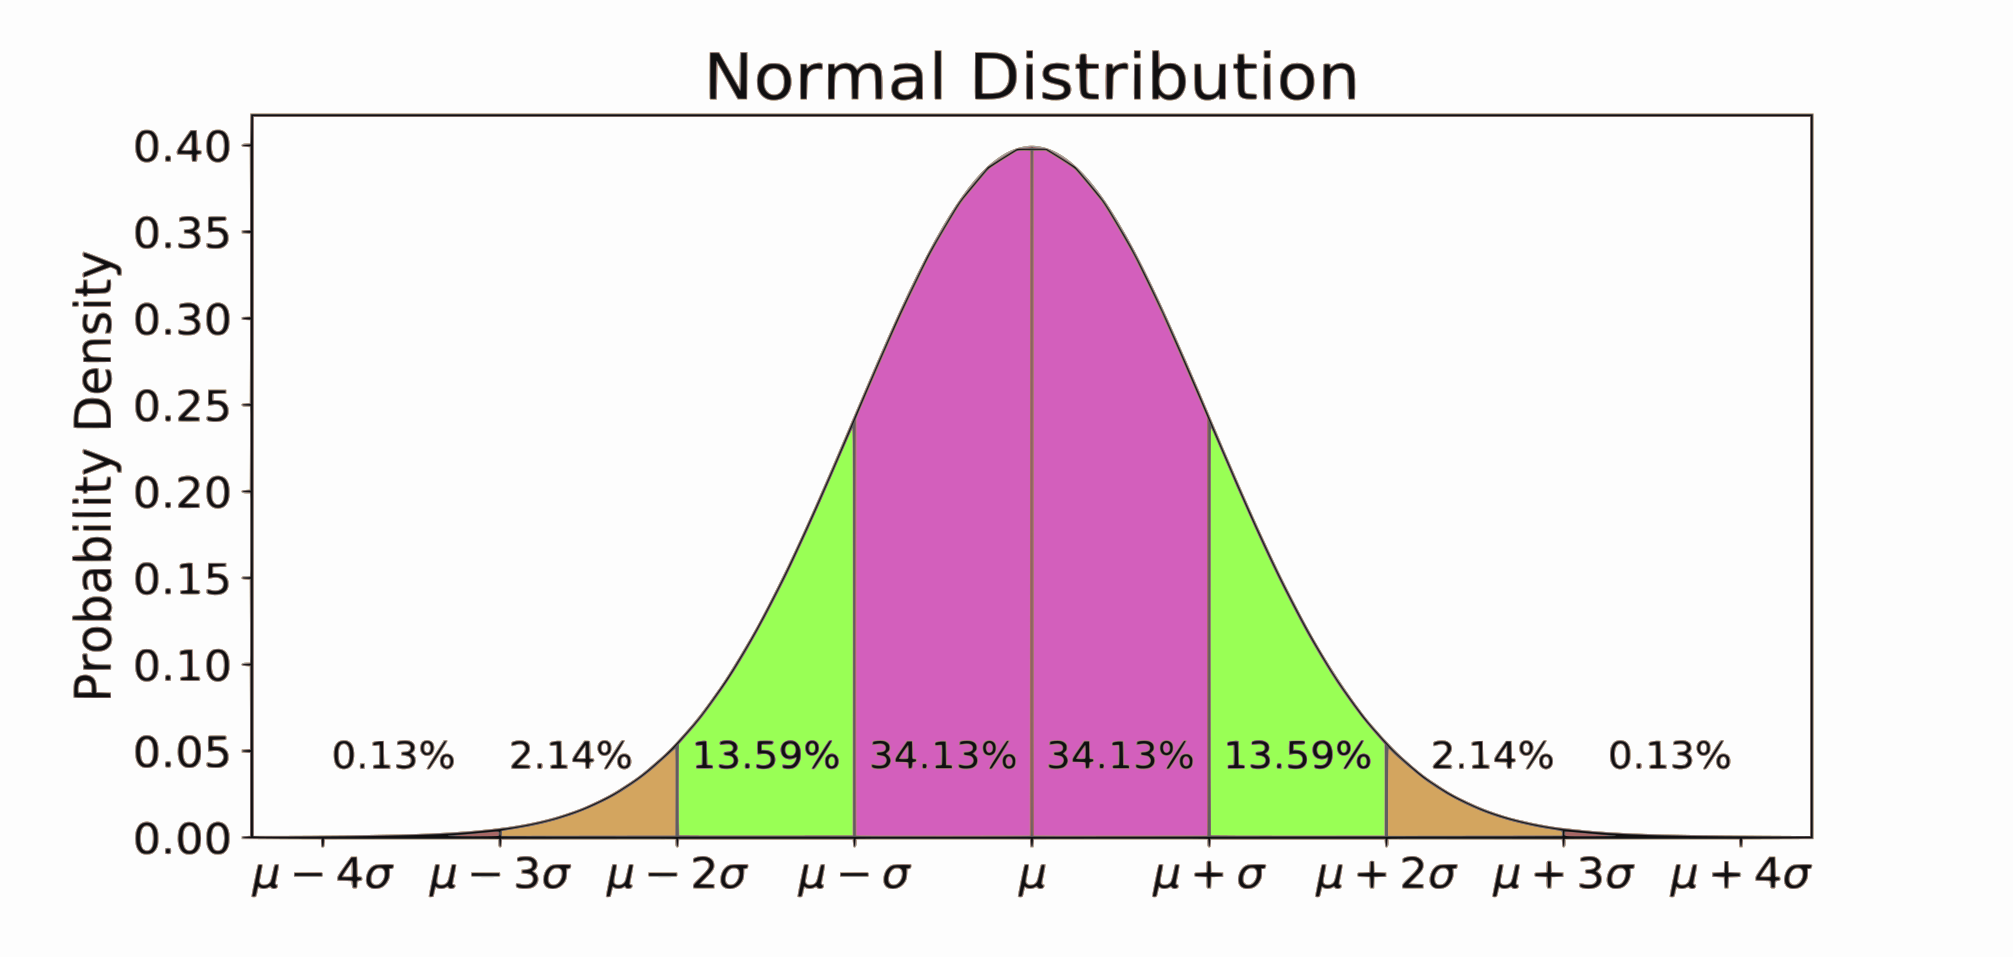
\includegraphics[width=5in]
{conventions/normal-dist.png}
\caption{Normal Distribution
$\caln(x;\mu, \s^2)$.}
\label{fig-norm-dist}
\end{figure}

The {\bf Standard Normal Distribution} $P_{SND}(x)$
and its cumulative distribution $\Phi(x)$ are defined by

\beq
P_{SND}(x)=\caln(x; \mu=0, \s=1)
\eeq

\beq
\Phi(x) = \int_{-\infty}^x dx'\;P_{SND}(x')
\eeq

The {\bf error function} ${\rm erf}:\RR\rarrow [-1,1]$
is defined by
\beq
{\rm erf}(x) = \frac{2}{\sqrt{\pi}}
\int_0^x du \; e^{-\;\frac{u^2}{2}}
\eeq

Note that

\beq
\Phi(x)= \frac{1}{2} + \frac{1}{2}{\rm erf}(x)
\label{eq-Phi-erf}
\eeq
Eq.(\ref{eq-Phi-erf})
is interpreted geometrically in Fig.\ref{fig-erf}.

\begin{figure}[h!]
\centering
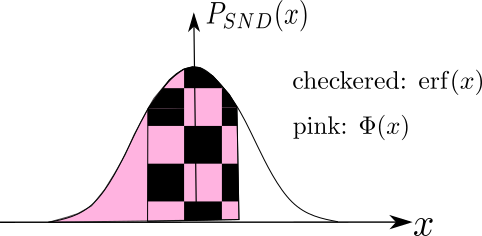
\includegraphics[width=2.8in]
{conventions/erf.png}
\caption{Plot of Standard
Normal Distribution $P_{SND}(x)$.
 Values of ${\rm erf}(x)$ and $\Phi(x)$
 equal indicated areas.}
 \label{fig-erf}
\end{figure}
\section{Uniform Distribution}
For $a<b$, $x\in [a,b]$

\beq
\calu(x;a,b) =
\frac{1}{b-a}
\eeq

\section {Softmax function
(a.k.a. Boltzmann Distribution)}

The Softmax function
 is defined by
\beq
P(x_i
|x.)=\frac{e^{x_i}}{\sum_i e^{x_i}}=
\softmax(x.)_i
\label{eq-softmax}
\eeq
The
Boltzmann distribution is defined as

\beq
P(\rvE_a=E_a)=\frac{\exp(-\;\frac{E_a}{kT})}{\sum_{a}
\exp(-\;\frac{E_{a}}{kT})}=
P(\frac{-E_a}{kT}|E.)\eeq
for a system with energies $E_a$
and temperature $T$,
where $k$
is Boltzmann's constant.

The function
softmax() is called softmax because if we
approximate the exponentials,
 both in the numerator and denominator
of Eq.(\ref{eq-softmax}),
by the largest one
of them or zero,
we get

\beq
\softmax(x.)_i\approx \indi(i=\argmax_k x_k)
\;.
\eeq
Thus, softmax($x.$)
returns a continuous
function that approximates a one-hot vector
that is 1 at the
$i$th
component, where
$i=\argmax_k(x_k)$,
and zero at the other components.

Note that
\beq
\pder{\ln P(x_i|x)}{x_a}
=
\pder{}{x_a}\ln\left[
\frac{e^{x_i}}{\sum_i e^{x_i}}
\right]
=
\delta(a,i)
-
P(x_a|x)
\eeq

For 2 variables $x_0, x_1$,
\beqa
P(x_0|x.)&=&
\frac{e^{x_0}}{e^{x_0} + e^{x_1}}\\
&=&\smoid(x_0-x_1)
\;,
\eeqa

\beq
P(x_1|x.)=\smoid(x_1-x_0)
\;.
\eeq

\section{Sigmoid and log-odds functions}
\label{sec0-smoid}
The {\bf sigmoid (a.k.a. exp-it,  logistic) function} smoid:$\RR\rarrow [0,1]$
is defined by
\beq
\smoid(x)=
\frac{1}{1+e^{-x}}
\eeq
$\smoid()$ is monotonically
increasing with $\smoid(-\infty)=0$,
$\smoid(0)=1/2$
and $\smoid(+\infty)=1$.
Note that for $x<<0$, $\smoid(x)\approx e^x$, which
is why ``smoid" is also called ``expit".

\beqa
\smoid(x)+\smoid(-x)&=&
\frac{1}{1+e^{-x}}+\frac{1}{1+e^x}\\
&=&\frac{2+e^x+e^{-x}}{2+e^x+e^{-x}}
\\&=&1
\eeqa


The {\bf log-odds (a.k.a. log-it) function}
lodds:$[0,1]\rarrow \RR$ is defined by

\beq
{\rm lodds}(p)=\ln\frac{p}{1-p}
\eeq
Note that for $0< p<<1$, $\lodds(x)\approx \ln p$,
which is why ``lodds" is also called ``logit".

Note that for $x<<1$, $\smoid(x)\approx e^x<<1$,
so $\lodds(e^x)\approx \ln(e^x)=x$.
More generally, it
is easy to check that for any $p\in[0,1]$ and $x\in \RR$,
\beq
\lodds[\smoid(x)]=x
\eeq

\beq
\smoid [\lodds(p)] =p
\eeq
Hence,
$\lodds()$ is the inverse of $\smoid()$ and vice-versa.

\begin{claim}
\beq
\smoid'(x)=\smoid(x)[1-\smoid(x)]
\eeq

\beq
\smoid''(x)=\smoid'(x)[1-2\smoid(x)]
\eeq
\end{claim}
\proof

In this proof, we will
abbreviate $\smoid(x)$ by $s(x)$.
\beq
1-s(x)=1 -\;\frac{1}{1+e^{-x}}=
\frac{e^{-x}}{1+e^{-x}}
\eeq

\beq
s'(x)= \frac{e^{-x}}{(1+e^{-x})^2}
=s(x)[1-s(x)]
\eeq

\beqa
s''(x)&=&s'(x)[1-s(x)]
+
s(x)(-1)s'(x)
\\
&=&
s'(x)[1-2s(x)]
\\
&=&
s(x)[1-s(x)][1-2s(x)]
\eeqa
\qed

\section{Estimand, Estimator (curve-fit, cfit), Estimate, Bias}
\label{sec0-estimand}
For an {\bf estimand} $\theta$,
an {\bf estimator (a.k.a. curve fit,
cfit)} $\ul{\HAT{\theta}}$
gives {\bf estimate} $E[\ul{\HAT{\theta}}(\theta)]=\theta+b$
with {\bf bias} $b$.
We say this estimate is an {\bf unbiased estimate}
if $b=0$.

Note that, strictly
speaking, an estimator is a function
waiting to be averaged over
and denoted by a letter with a hat,
whereas an estimate is a real number
denoted by a letter without a hat.
Unfortunately, the
words ``estimator" and
``estimate" are often used interchangeably,
as if they were synonyms.
And often the estimate $\theta + b$
is denoted by a letter with a hat too.
In some sense, an estimator is an estimate
of a curve, so it's understandable that
the terms ``estimator" and ``estimate"
are used synonymously.
In this book, we will bow to traditional
practice and
also use
the terms ``estimator" and ``estimate"
synonymously, and use a letter
with a hat to denote either of them.
This is not
ambiguous as long as we don't
use the same letter with a
hat to denote two different quantities, of course.
When we need to distinguish semantically
between the real value and the function,
we will call the function a cfit,
and the real value the estimate.

\section{Maximum Likelihood Estimate,
Likelihood Ratio Test}
\label{sec0-likelihood-ratio}

Given a bnet, let $P(x|\theta)$
be its full joint probability distribution,
where
$x$ denotes the joint state
of all the nodes and $\theta$
denotes all the parameters.
 $P(x|\theta)$ is often
called the {\bf likelihood function of $\theta$}
and is denoted by

\beq
L(\theta)= P(x|\theta)
\eeq
It's called a likehood of $\theta$
because, even though it's a probability,
it isn't the probability of $\theta$,
but rather of $x$.

The value of $\theta$
that we obtain by maximizing $L(\theta)$
over $\theta$ is called
the
{\bf maximum likelihood
estimate (MLE) of $\theta$}. Let us denote it by
$\HAT{\theta}$. Note that\footnote{``sup" stands for supremum.
It's a generalization of the function $\max()$
to arbitrary sets
that might not be discrete or finite.
If $S$ is a
finite set,
then $\sup_{\theta\in S} f(\theta)=
\max_{\theta\in S} f(\theta)$
for any function $f:S\rarrow \RR$.
Likewise, ``inf" stands for infimum,
and it generalizes the $\min()$ function.}

\beq
\sup_{\theta\in S}L(\theta)=
L(\HAT{\theta})
\eeq


Let $S_0, S_1$ be disjoint sets such that
 $S=S_0\cup S_1$.
We'll say
the {\bf null hypothesis $H_0$} holds
 if $\theta\in S_0$,
and the {\bf alternative hypothesis $H_1$}
holds if
$\theta\in S_1$.
The {\bf likelihood ratio (LR) test statistic}
is defined by


\beq
R=-2\ln
\left(\frac{\sup_{\theta\in S_0}L(\theta)}
{\sup_{\theta\in S}L(\theta)}\right)
\eeq
$R\geq 0$ and $R=0$ if  $S_0=S$.
For some small $c>0$,
if $R<c$, then we reject the alternative hypothesis,
and if $R>c$, we accept it.




If $S_0=\{\theta_0\}$,
then

\beq
R= -2[\ln L(\theta_0) -\ln L(\HAT{\theta})]
\eeq


\section{Mean Square Error (MSE)}

Suppose we are
given $nsam$ samples $y^\s\in\RR$
labeled by an index $\s$,
and a cfit $\haty^\s(a)\in\RR$
that depends on a parameter $a\in\RR$.
Define the {\bf Mean Square
Error (MSE)}
by

\beq
MSE(a) = \frac{1}{nsam}\sum_\s (y^\s-\haty^\s(a))^2
\;.
\eeq
For example, in Linear Regression (LR),
we have $\haty^\s= a_0 + a_1 x^\s$
where $a=(a_0, a_1)$ is a deterministic
parameter.
If the samples $y^\s$
are i.i.d,
then we can also write


\beq
MSE(a)=E_{|a}[(\rvy-\ul{\haty}(a))^2]
\;.
\eeq
and for LR, $\ul{\haty}(a)=a_0+a_1\rvx$.

Define the {\bf residual} $\Delta\rvy$ by:


\beq
\Delta\rvy(a) =\rvy-\ul{\haty}(a)
\;\;\;\text{ (Hence
$\rvy=\ul{\haty} + \Delta\rvy$)}
\eeq

In the rest of this section,
we will discuss the case that
$\haty^\s(a)$ is independent of $x^\s$.
I call
this the {\bf deterministic MSE (D-MSE)}
model.
Note that this
is different from the LR
case where
$\haty^\s(a)$ does depend on $x^\s$.
In LR, we are trying
to fit
a line to a cigar-shaped
2-D scatter plot.
Here, we are just trying
to estimate
the mean value (center of mass)
of a scatter plot.


\begin{claim}
MSE is minimized
over all functions $\haty$ if
\beq
\haty =E_{|a}[\rvy]
\eeq
\end{claim}
\proof

\beq
MSE = E_{|a}[\rvy^2]-2\haty E_{|a}[\rvy]+ \haty^2
\eeq

\beq
0=\frac{d}{d\haty} MSE = 2(-E_{|a}[\rvy]+\haty)
\eeq
Hence,
\beq
\haty =E_{|a}[\rvy]
\eeq
\qed

Sometimes, we will
use the notation
\beq
\haty_{MSE} = E_{|a=a_{MSE}}[\rvy]
\;.
\eeq

\begin{claim}
Suppose $f(a)$
is a function of $a$.
If $\haty=E_{|a}[\rvy]$, then

\beq
E_{|a}[\Delta \rvy]=
E[\Delta \rvy]=0
\eeq



\beq
E_{|a}
\left[\Delta \rvy f(\rva)\right]=
E
\left[\Delta \rvy f(\rva)\right]=0
\eeq
\end{claim}
\proof

\beq
E_{|a}[\Delta\rvy]=
E_{|a}
\left[\rvy-E_{|a}[\rvy]\right]=
E_{|a}[\rvy]-E_{|a}[\rvy]=0
\eeq

\beq
E[\Delta \rvy] =
 E_{\rva}[E_{|\rva}[\Delta\rvy]]=0
\eeq


\beqa
E_{|\rva}
\left[\Delta \rvy f(\rva)\right]
&=&
f(\rva)
\underbrace{E_{|\rva}
[\Delta\rvy]}_{=0}
\eeqa

\beq
E[\Delta \rvy f(\rva)]
=E_\rva[E_{|\rva}[\Delta\rvy f(\rva)]]=0
\eeq
\qed


\begin{claim}
If $\haty=E_{|a}[\rvy]$, then

\beq
\av{\Delta\rvy, \haty}_{|a}
=0
\label{eq-mse-uncorr}
\eeq

\beq
Var_{|a}[\rvy]
=
Var_{|a}[\haty]
+
Var_{|a}[\Delta\rvy]
\eeq
The same results hold
without the conditioning on $a$.
\end{claim}
\proof

\beqa
\av{\Delta\rvy, \ul{\haty}}_{|a}
&=&
\underbrace{E_{|a}[\Delta\rvy \;\underbrace{\ul{\haty}}
_{f(\rva)}]
}_{=0}
-
\underbrace{E_{|a}[\Delta\rvy]}_{=0}
E_{|a}[ \ul{\haty}]
\eeqa

\beqa
Var_{|a}[\rvy]
&=&
\av{\haty +\Delta\rvy, \haty +\Delta\rvy}_{|a}
\\
&=&
\av{\haty, \haty}_{|a}
+
\av{\Delta\rvy, \Delta\rvy}_{|a}
\;\text{(by Eq.(\ref{eq-mse-uncorr}))}
\\
&=&
Var_{|a}[\haty]
+
Var_{|a}[\Delta\rvy]
\eeqa
The same proof
holds
if we remove all the $|a$
subscripts.
\qed

Fig.\ref{fig-ms-error}
illustrates how
$\rvy=\ul{\haty} +\Delta \rvy$
and the variances of these
quantities add.


\begin{figure}[h!]
\centering
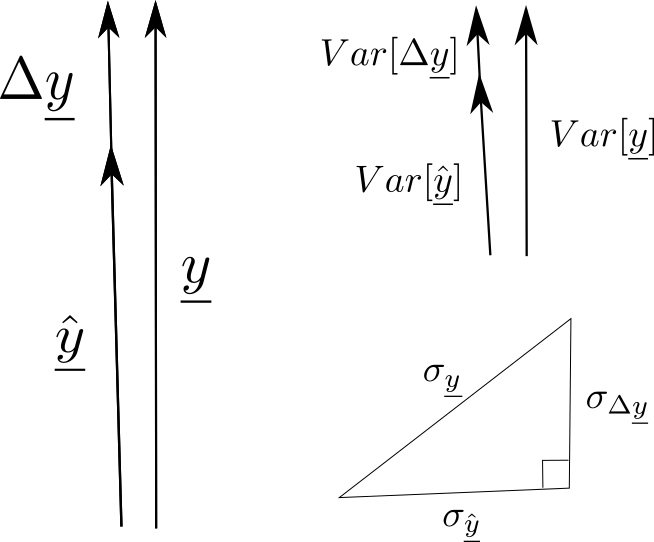
\includegraphics[width=2.3in]
{conventions/ms-error.png}
\caption{$\rvy=\HAT{y}+\Delta y$
and the variances (not standard deviations)
of these quantities add. }
\label{fig-ms-error}
\end{figure}

\section{Cramer-Rao Bound}

This discussion of the Cramer-Rao (CR) bound
is based on Ref.\cite{wiki-cramer-rao}.

Suppose $\rvx$ is a random variable with values $x\in S_\rvx$
and $\theta\in\RR$ is a parameter.
For any function
$f_{\rvx,\theta}: S_\rvx\times \RR\rarrow \RR$,
define

\beq
\av{f_{\rvx,\theta}} =\sum_x P(x|\theta)f_{x,\theta}
\eeq

\beq
\Delta f_{\rvx,\theta}=f_{\rvx,\theta}-\av{f_{\rvx,\theta}}
\eeq

\beq
\av{f_{\rvx,\theta},f_{\rvx,\theta}}=
\av{\Delta f_{\rvx,\theta}\;\Delta f_{\rvx,\theta}}
\eeq

Define the {\bf log likelihood function} by
\beq
LL_\theta = \ln P(x|\theta)
\eeq

Define the {\bf Fisher information} by
\beq
I_\theta=\av{\partial_\theta LL_\theta,\partial_\theta LL_\theta}
\eeq

Note that $LL_\theta\leq 0$.
Let $\theta^*$ be the
value of $\theta$ that maximizes $LL_\theta$.


Note that $I_\theta\geq 0$ and
$I_\theta=0$ when $\theta=\theta^*$
because $\partial_\theta LL_\theta|_{\theta=\theta^*}=0$.
This suggests that $I_\theta$
measures the distance
between $\theta$ and $\theta^*$.



Note that
\beqa
\av{\partial_\theta LL_\theta}&=&
\sum_x P(x|\theta)\frac{1}{P(x|\theta)}
\partial_\theta P(x|\theta)
\\
&=&
\partial_\theta \sum_x P(x|\theta)
\\
&=&
0
\eeqa
Therefore

\beqa
I_\theta &=&\av{[\partial_\theta LL_\theta]^2}
-
\av{\partial_\theta LL_\theta}^2
\\
&=&
\av{[\partial_\theta LL_\theta]^2}
\eeqa

\begin{claim}
\beq
I_\theta = -\av{\partial_\theta^2 LL_\theta}
\eeq
\end{claim}
\proof

\beqa
I_\theta &=& \av{[\partial_\theta LL_\theta]^2}
\\
&=&
\sum_x P(x|\theta)
\frac{1}{P(x|\theta)}
\partial_\theta P(x|\theta)
\partial_\theta \ln P(x|\theta)
\\
&=&
-\sum_x P(x|\theta)\partial_\theta^2 \ln P(x|\theta)
+ \partial_\theta\sum_x
P(x|\theta)\partial_\theta \ln P(x|\theta)
\\
&=&
-\av{\partial_\theta^2 LL_\theta}
+ \partial_\theta^2\sum_x P(x|\theta)
\\
&=&
-\av{\partial_\theta^2 LL_\theta}
\eeqa
\qed

\begin{claim}
If $x=[x_i]_{i=1,2, \ldots \nu}\in \RR^\nu$ are i.i.d., then


\beq
I_\theta = \nu \av{[\partial_\theta LL_{\theta, i}]^2}
\eeq
where

\beq
LL_{\theta, i} = \ln P(x_i|\theta)
\eeq
\end{claim}
\proof

\beqa
LL_\theta
&=& \ln \prod_i P(x_i|\theta)
\\
&=&
\sum_i LL_{\theta, i}
\eeqa

\beqa
I_\theta &=&
\sum_i \sum_j \av{
\partial_\theta LL_{\theta,i}
\partial_\theta LL_{\theta,j}
}
\\
&=&
\sum_i  \av{
[\partial_\theta LL_{\theta,i}]^2}
\\
&=&
\nu \av{
[\partial_\theta LL_{\theta,i}]^2
}
\eeqa
\qed




A function  $t_\rvx:S_\rvx\rarrow \RR$
is called a {\bf test statistic} of random variable $\rvx$.

\begin{claim}(Cramer-Rao bound for single parameter $\theta\in\RR$)

\beq
\av{t_\rvx,t_\rvx}I_\theta \geq
 \left[\partial_\theta\av{t_\rvx}\right]^2
 \label{eq-crao-tx}
 \eeq
\end{claim}
\proof

Cauchy-Schwartz inequality

For two vectors $\veca,\vecb\in\RR^n$:
\beq
\veca\cdot\vecb =|\veca||\vecb|\cos \phi \leq |\veca||\vecb|
\eeq

For two real valued random variables $\rva, \rvb$:
\beq
\av{\rva, \rva} \av{\rvb,\rvb}\geq |\av{\rva,\rvb}|^2
\eeq
Replace

\beq
\rva\rarrow t_\rvx,
\quad\rvb\rarrow \partial_\theta LL_\theta
\eeq
Then

\beqa
\av{t_\rvx, \partial_\theta LL_\theta}
&=&
\av{t_\rvx \partial_\theta LL_\theta}
-
\av{t_\rvx} \underbrace{\av{\partial_\theta LL_\theta}}_{=0}
\\
&=&
\sum_x P(x|\theta)
t_\rvx \frac{1}{P(x|\theta)}\partial_\theta P(x|\theta)
\\
&=&
\partial_\theta\sum_x  t_\rvx P(x|\theta)
\\
&=&
\partial_\theta\av{ t_\rvx}
\eeqa
\qed

See Fig.\ref{fig-cramer-rao}
for a pictorial representation
of Eq.(\ref{eq-crao-tx}).

\begin{figure}[h!]
\centering
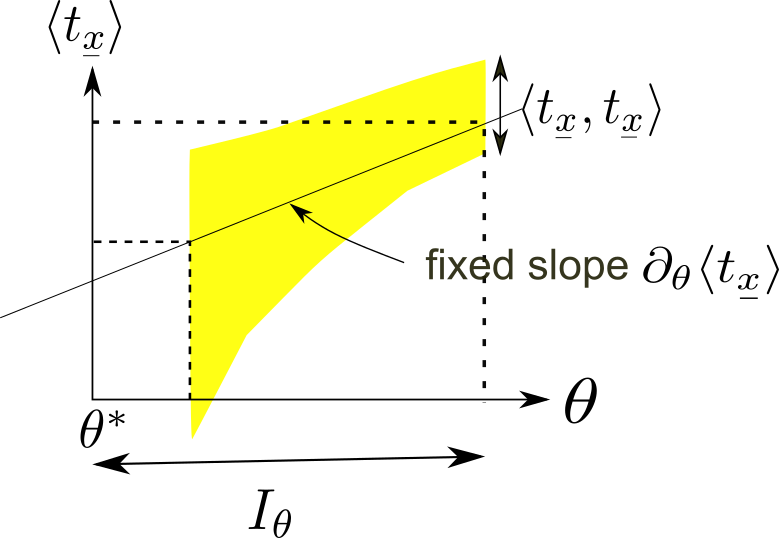
\includegraphics[width=2.7in]
{conventions/cramer-rao.png}
\caption{
In this drawing,
$\theta^*$ is the
value of $\theta$ that maximizes $LL_\theta$.
According
to the CR bound,
the product of the
variance $\av{t_\rvx, t_\rvx}$ and
the distance $I_\theta$
must be greater or equal to $[\partial_\theta\av{t_\rvx}]^2$.
At fixed $[\partial_\theta\av{t_\rvx}]^2$,
if the variance increases, the distance decreases,
and vice versa.
}
\label{fig-cramer-rao}
\end{figure}


Now suppose the test statistic $t_\rvx$
equals an {\bf estimator} $\HAT{\theta}$
of $\theta$ with bias $b_\rvx:S_\rvx \rarrow \RR$.

\beq
t_\rvx = \HAT{\theta}(\rvx) = \theta + b_\rvx
\eeq
$\HAT{\theta}$ is said to be a {\bf biased estimator}
if $b_\rvx\neq 0$ and an {\bf unbiased estimator} if $b_\rvx=0$.

\begin{claim}

\beq
\av{\HAT{\theta}} = \theta + \av{b_\rvx}
\eeq

\beq
\av{\HAT{\theta}, \HAT{\theta}} \geq
\frac{[1 + \partial_\theta\av{b_\rvx}]^2}
{I_\theta}
\label{eq-crao-theta}
\eeq

\beq
\av{[\HAT{\theta}-\theta]^2} \geq
\frac{[1 + \partial_\theta\av{b_\rvx}]^2}
{I_\theta}
+
\av{b_\rvx}^2
\eeq

\end{claim}
\proof
\beqa
\partial_\theta\av{t_\rvx}
&=&
\partial_\theta\av{\theta + b_\rvx}
\\
&=&
\partial_\theta\left[\theta +\av{b_\rvx}\right]
\\
&=&
1 + \partial_\theta\av{b_\rvx}
\eeqa
Eq.(\ref{eq-crao-theta})
follows from Eq.(\ref{eq-crao-tx})
once we replace $t_\rvx$ by $\HAT{\theta}$.

Let
\beq
\Delta \HAT{\theta} =
\HAT{\theta} -\av{\HAT{\theta}}
=
\underbrace{(\HAT{\theta} -\theta)}_\xi  - \av{b_\rvx}
\eeq
Then

\beq
0=\av{\Delta \HAT{\theta}} = \av{\xi} - \av{b_\rvx}
\eeq

\beqa
\frac{[1 + \partial_\theta\av{b_\rvx}]^2}
{I_\theta} &\leq&
\av{[\Delta \HAT{\theta}]^2}
\\
&=&
\av{\xi^2 -2\xi\av{b_\rvx} + \av{b_\rvx}^2}
\\
&=&
\av{\xi^2} -\av{b_\rvx}^2
\eeqa

\qed

Multi-dimensional case:
parameter
 $\theta=[\theta_1, \theta_2, \ldots, \theta_n]^T\in \RR^n$
 and test statistic
 $t_\rvx=[t_{\rvx,1}, t_{\rvx,2}, \ldots, t_{\rvx,n}]^T\in \RR^n$
are column vectors.

Define {\bf Fisher information matrix} by

\beq
[I_\theta]_{i,j}=
\av{\partial_{\theta_i} LL_\theta, \partial_{\theta_j}LL_\theta}
=
\av{\partial_{\theta_i} LL_\theta\;\partial_{\theta_j}LL_\theta}
\eeq

CR bound for multi-dimensional parameter $\theta\in\RR^n$:
\beq
\text{matrix}\left[\av{t_{\rvx,i}, t_{\rvx,j}}\right]\geq
\text{matrix}\left[
\partial_{\theta_i} \av{t_{\rvx,a}}
[I_\theta]^{-1}_{a,b}
\partial_{\theta_j} \av{t_{\rvx,b}}
\right]
\eeq
where we are using the Einstein summation
convention (repeated indices are summed over).
For two matrices $A,B\in\RR^n$, $A\geq B$ means $A-B$ has
non-negative eigenvalues.


\section{Bayes Rule,
Bayesian Updating And Conjugate Priors}

Bayes Rule says:

\beq
P(\theta|x)P(x)
=
P(x|\theta)P(\theta)
\eeq
Expressed diagramatically\footnote{Two bnets are equated if their full probability
distributions (i.e.,
their full instantiations) are equal numerically.
For example,  
$$
\rva\rarrow\rvb\rarrow \rvc = P(c|b)P(b|a)P(a)= \rva\larrow\rvb\larrow\rvc
$$},
we have for  $\rvx\in\RR$:
\beq
\xymatrix{
\rvtheta&\rvx\ar[l]
}
\quad =\quad
\xymatrix{
 \rvtheta\ar[r]&\rvx
}
\eeq
and for $\rvx=(\rvx_1, \rvx_2)\in \RR^2$:
\beq
\begin{array}{c}
\xymatrix@R=.3pc{
&\rvx_1\ar[ld]\ar[dd]
\\
\rvtheta
\\
&\rvx_2\ar[lu]
}
\xymatrix@R=.3pc{\\\quad =\quad}
\xymatrix@R=.3pc{
&\rvx_1\ar[dd]
\\
\rvtheta\ar[ru]\ar[rd]
\\
&\rvx_2
}
\end{array}
\eeq
Note how Bayes rule
allows us to reverse the
direction of the arrows
impinging on $\theta$.
We see from Bayes Rule
that even though
the directions of
the arrows in a
bnet can have causal
motivation, a bnet
with arrows reversed
from their causally
motivated directions
can still be very useful
as a calculation tool.

Another way of stating
Bayes Rule is




\beq
\underbrace{P(\theta|x)}_{\rm posterior}=
\caln(!\theta)
\underbrace{P(x|\theta)}_{\rm likelihood}
\underbrace{P(\theta)}_{\rm prior}
\;.
\eeq

If, for a given likelihood,
the prior and posterior
distributions belong to
the same family (for instance,
they are both
Beta distributions),
then we say that the prior is the
{\bf conjugate prior}
of that likelihood.

For example,
Beta $\sim$ Bernoulli*Beta.
Hence, the
Beta distribution\footnote{See
Ref.\cite{wiki-beta-dist} for a discussion
of the Beta distribution.}
is the conjugate prior of the
Bernoulli distribution\footnote{See
Ref.\cite{wiki-bern-dist} for a discussion
of the Bernoulli distribution}.
More explicitly,
if

\beq
p_1\sim {\rm Beta}(p_1;\alp, \beta)
\eeq
and

\beq
x|p_1\sim {\rm Bernoulli}(x;p_1)
\;,
\eeq
where $p_1=P(x=1)$,
then

\beq
p_1|x\sim {\rm Beta}(p_1;\alp', \beta')
\eeq
where

\beq
\alp'= \alp + x
\eeq

\beq
\beta'= \beta + (1-x)
\eeq


Ref.\cite{wiki-conj-prior}
has a table of
conjugate priors.

Conjugate priors facilitate
Bayesian updating
of the prior to
posterior in a
feedback loop(see Fig.\ref{fig-conj-prior}).

\begin{figure}[h!]
$$\xymatrix{
&x_t\ar[d]
\\
&\stackrel{Bernoulli}{P(x_t|\theta)}\ar@/_2pc/[ld]
\\
\stackrel{Beta}{P(\theta|x_{\leq t})}\ar@/_2pc/[rd]
&&\stackrel{Beta}{P(\theta|x_{\leq t-1})}\ar@/_2pc/[ul]
\\
&t\rarrow t+1 \text{ for } t=0, 1, 2,\ldots
\ar@/_2pc/[ur]
}$$
\caption{Bayesian updating facilitated
by conjugate prior. In this figure,
$x_{\leq t}=(x_0, x_1, \ldots, x_{t-1}, x_t)$.}
\label{fig-conj-prior}
\end{figure}


\section{Linear regression, Ordinary Least Squares (OLS)}
\label{sec0-conv-lr}
Wikipedia articles
\begin{enumerate}
\item
Linear Regression (LR)
\begin{itemize}
\item
linear regression, Ref.\cite{wiki-lr}
\item
 simple linear regression, Ref.\cite{wiki-slr}
\item
errors in variable, Ref.\cite{wiki-errors-in-iv}

\end{itemize}
\item
Least squares (LS)
\begin{itemize}
\item
least squares, Ref.\cite{wiki-lsquares}
\item
ordinary least squares (OLS), Ref.\cite{wiki-ols}
\end{itemize}
\end{enumerate}


Some nomenclature: In LR, the
data consists of
{\bf independent x-variables} $x^\s_1,
 x^\s_2, \ldots x^\s_n$
and a {\bf dependent y-variable} $y^\s$.
We find a linear fit $\haty^\s =
\beta_0 + \sum_{i=1}^n \beta_i x^\s_i$
to the data.
$\haty^\s$ is called the {\bf estimate}
of $y^\s$.
 The coefficients $\beta_0, \beta_i$
are called {\bf regression coefficients}.
$y^\s-\haty^\s=\eps^\s$
are called  the {\bf residuals}.
$\cale =\sum_\s (\eps^\s)^2$
is called the {\bf error or cost}. We choose the
regression coefficients
so as to minimize the error.

Below, we consider two types of LR:

\begin{enumerate}
\item
LR
in which the independent x-variables are non-random.
\item
LR
in which the independent x-variables are random
and i.i.d.
\end{enumerate}

The  term OLS
is often used to refer to LR
of type 1.



For LR of type 2,
there is randomness in $y$
coming from the randomness in $x$
and in the residuals.
For LR of type 1,
there  is randomness in $y$
too, but
it comes
from the residuals
only.

Once one assumes that certain
variables are random, a
``model" (i.e., a bnet,
with probabilities expressed as TPMs)
 must be
specified.


\subsection{LR, assuming
$x_\s$ are non-random}

Let

$\s\in\{0, 1, 2, \ldots, nsam-1\}$ : sample index

$i_0\in\{0, 1, 2, \ldots, n\}$ :
index that can assume values 0 to $n$

$i\in\{1, 2, \ldots, n\}$ :
index that can assume values 1 to $n$.
$i$ is never equal to 0.


$y_\s\in \RR$: dependent y-variables

$x_{\s i}\in \RR$: independent x-variables

$\eps_\s\in \RR$: residuals

$\beta_0, \beta_i\in \RR$:
regression coefficients


\beq
y_\s= \beta_0 +
\sum_{i=1}^{n} x_{\s i}\beta_{i} + \eps_\s
\label{eq-LR-start}
\eeq

If we define
\beq
x_{\s 0}=1
\;
\eeq
for all $\s$, then

\beq
y_\s=
\sum_{i_0=0}^{n} x_{\s i_0}\beta_{i_0} + \eps_\s
\;.
\eeq
If $y$ and $\eps$ are $nsam$ dimensional
 column vectors and $\beta$
is an $n+1$ dimensional column vector,
and $X$ is an $nsam\times (n+1)$ matrix,
then we can write the previous equation in matrix
form as:


\beq
y=X\beta+\eps
\;.
\eeq

\subsubsection{Derivation of LR
 From Minimization of Error}

Let $W=[W_{\s, \s'}]$
be a symmetric matrix with non-negative
diagonal elements $W_{\s,\s}\geq 0$ for all $\s$.
$W$ is called the {\bf weight matrix}.
The following claim
describes the method of
{\bf Weighted LR}
when $W\neq 1$
and of simple LR  when $W=1$.
\begin{claim}
Assume the
Einstein summation convention; i.e.,
implicit sum over
repeated indices.
The
 error function $\cale$ given by

\beq
\cale=
\underbrace{(y_{\s}-X_{\s, j_0}\beta_{j_0})}
_{\text{residual $\eps_\s$}}
W_{\s, \s'}
\underbrace{(y_{\s'}-X_{\s', k_0}
\beta_{k_0})}_{\eps_{\s'}}
\;,
\eeq
is minimized
over $\beta_{k_0}$ for all $k_0
\in\{0,1,\ldots,n\}$,
if $\beta_{k_0}$ is given by:

\beq
\HAT{\beta}= (X^T W X)^{-1} X^T W y
\;.
\label{eq-betahat-non-ran-w}
\eeq
When $W=1$,

\beq
\HAT{\beta}= (X^T X)^{-1} X^T y
\;.
\label{eq-betahat-non-ran}
\eeq

\end{claim}
\proof

At the minimum of $\cale$,
the variation $\delta\cale$
 must vanish:
\beq
0=\delta \cale=
-2 X_{\s j_0}(\delta \beta_{j_0})
W_{\s, \s'}(y_{\s'}
-X_{\s' k_0}
\beta_{k_0})
\;.
\eeq
Thus,

\beq
X^T W y - X^T W X\beta=0
\eeq
which
implies Eq.(\ref{eq-betahat-non-ran-w}).
\qed

\subsubsection{Geometry of LR
with non-random $x_\s$.}

Recall that

\beq
y=X\beta+\eps
\;.
\eeq


Define the {\bf projection matrices}

\beq
\A=X(X^TX)^{-1}X^T
\;,\;\;\V=1-\A
\eeq
A square matrix $M$
is symmetric if $M^T=M$
and is idempotent if $M^2=M$.
$\A$ is symmetric
and idempotent
and so is $\V$.
Note that $\A$ and $\V$
also satisfy:

\beq
\V\A=\A\V=0
\eeq
and

\beq
\A X=X\;,\;\; \V X=0
\;.
\eeq

One has

\beq
\beta=
(X^TX)^{-1}X^T(y-\eps)
\;.
\eeq


Define

\begin{subequations}
\beq \boxed{
\HAT{\beta}=
\underbrace{(X^TX)^{-1}X^T}_B \;y
\;,
}
\label{eq-beta-nonrandom-lin-reg}
\eeq



\beq
\HAT{y}=
X\HAT{\beta}= \A y
\;,
\eeq
and

\beq
\HAT{\eps}=
y-X\HAT{\beta}=
y-\HAT{y}=(1-\A)y=\V y
\;.
\eeq
\end{subequations}
$\A$ is sometimes  called the {\bf hat matrix},
because it gives $y$ a hat.

Given any function $f=f(y,X,\eps)$
and a scalar factor $\xi\in \RR$,
suppose
$f(\xi y, \xi X, \xi\eps)=\xi^\calo f(y,X,\eps)$.
Then we will say that $f(\cdot)$
is of {\bf order $\calo$ under scaling}.
Note that $\{\HAT{y},
 \HAT{\eps}\}$
are all of order 1 under scaling,
$\{\beta, \HAT{\beta}, \A, \V\}$
are all of order 0 under scaling,
and $B$ is of order $-1$ under scaling.
Thus, each cfit (i.e., symbol
with a hat)
scales the same way as its estimand (i.e., same
symbol
without a hat). Furthermore,
$\beta$, its cfit $\HAT{\beta}$, and
the projection matrices $\A, \V$
are invariant ($\calo=0$) under scaling.



Note that $y$
can be expressed as
a sum of 2 orthogonal estimates:



\beq
y= \underbrace{\HAT{y}}_{\A y} +
\underbrace{\HAT{\eps}}_{\V y}
\;.
\eeq
Fig.\ref{fig-lin-reg-vecs}
shows triangles representing
$y=X\beta+\eps$ and $y=\HAT{y}+\HAT{\eps}$.


\begin{figure}[h!]
\centering
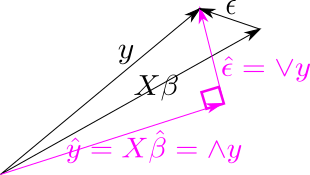
\includegraphics[width=2in]
{conventions/lin-reg-vecs.png}
\caption{Triangles
representing
$y=X\beta+\eps$ and $y=\HAT{y}+\HAT{\eps}$.}
\label{fig-lin-reg-vecs}
\end{figure}

\subsubsection{LR Goodness of Fit, $R^2$}


Assume the components of $\eps$
are random with zero mean:

\beq
E[\rveps]=\av{\rveps}=0
\eeq



Assume $X$ and $\beta$ are not random.
This makes $\rvy=X\beta +\rveps$ and $\ul{\HAT{\beta}}=
(X^TX)^{-1}X^T\rvy
$
random.
One finds that

\begin{subequations}
\beq
\av{\rvy}=X\beta
\eeq


\beq
\av{\HAT{\rvy}}=\A
\underbrace{\av{\rvy}}_{X\beta}
=\av{\rvy}
\eeq

\beq
\av{\HAT{\rveps}}=\V
\underbrace{\av{\rvy}}_{X\beta}
=0
\eeq

\beq
\av{\ul{\HAT{\beta}}}=\beta
\eeq


So far, we have
assumed a zero mean value for $\eps$.
Next, assume
{\bf  ``homoscedasticity" (homo-spread)}\footnote{I
 find the word ``homoscedasticity"
unnecessarily long, cryptic
and easy to misspell so
I like to replace
it by ``homo-spread".
The opposite
of ``homoscedasticity"
is ``heteroscedasticity",
which I like to replace with ``hetero-spread".}, which
means that

\beq
\av{\rveps, \rveps^T}=\xi^2 I_{nsam}
\eeq
\end{subequations}
where
$\xi\geq 0$,  and
$I_{nsam}$ is the
$nsam\times nsam$ identity matrix.
It follows that

\begin{subequations}
\label{eq-lin-re-variances}
\beq
\av{\rvy, \rvy^T}=
\av{\rveps, \rveps^T}=
\xi^2 I_{nsam}
\;,
\eeq

\beq
\av{\HAT{\rveps},
\HAT{\rveps}^T}=
\V\av{\rvy, \rvy^T}\V^T=\xi^2\V
\label{eq-homo}
\;,
\eeq

\beq
\av{\HAT{\rvy},
\HAT{\rvy}^T}=
\A\av{\rvy, \rvy^T}\A^T=\xi^2\A
\eeq
and

\beq
\av{\HAT{\ul{\beta}},
\HAT{\ul{\beta}}^T}=
B\av{\rvy, \rvy^T}B^T=\xi^2 (X^TX)^{-1}
\;.
\eeq
\end{subequations}

For any random column vector $\rva$,
let

\beq
\norm{\rva}^2= \rva^T\rva=\tr(\rva\rva^T)
\eeq
and

\beq
\av{\norm{\rva-\av{\rva}}^2}=
\av{\rva^T\rva}-\av{\rva^T}\av{\rva}
=
\tr\av{\rva, \rva^T}
\;.
\eeq

Define the following sums of squares (SS):

\begin{subequations}
\label{eq-lin-reg-ss}
\beq
SS_{\rvy}=\av{\norm{\rvy-\av{\rvy}}^2}
=\av{\rvy^T\rvy}-\av{\rvy^T}\av{\rvy}
=\tr\av{\rvy,\rvy^T}
\eeq

\beq
SS_{\HAT{\rvy}}=\av{\norm{\HAT{\rvy}-\av{\HAT{\rvy}}}^2}
=\av{\HAT{\rvy}^T\HAT{\rvy}}-\av{\HAT{\rvy}^T}\av{\HAT{\rvy}}
=\tr\av{\HAT{\rvy},\HAT{\rvy}^T}
\eeq

\beq
SS_{res}=\av{\norm{\rvy-\HAT{\rvy}}^2}
=
\av{\norm{\ul{\HAT{\eps}}}^2}
=\tr\av{\ul{\HAT{\eps}},\ul{\HAT{\eps}}^T}
\eeq
\end{subequations}

\begin{claim}
The following is true
without homo-spread:


\beq
\underbrace{\tr\av{\rvy,\rvy^T} }_{SS_\rvy}
=
\underbrace{\tr\av{\HAT{\rvy}, \HAT{\rvy}^T}}_{SS_{\HAT{\rvy}}}
+
\underbrace{\tr\av{\HAT{\rveps}, \HAT{\rveps}^T}}_{SS_{res}}
\eeq
This is like the Pythagorean Theorem
for the magenta right triangle
in Fig.\ref{fig-lin-reg-vecs}.
\end{claim}
\proof

From Eqs.\ref{eq-lin-re-variances}
and \ref{eq-lin-reg-ss},
we see that

\beq
SS_\rvy=\tr\av{\rvy,\rvy^T}
\eeq

\beq
SS_{\HAT{\rvy}}=\tr\av{\HAT{\rvy},\HAT{\rvy}^T}
=\tr\av{\A\rvy, \rvy^T}
\eeq

\beq
SS_{res}=\tr\av{\HAT{\rveps}, \HAT{\rveps}^T}
=\tr\av{\V\rvy, \rvy^T}
\eeq
Now use $\A + \V=1$.
\qed


The goodness of fit
for this model
is often measured using  the
{\bf coefficient of determination}
$R^2$. $R^2$  is defined by


\beq
R^2= 1 -\;\frac{SS_{res}}{SS_\rvy}=
\frac{SS_{\HAT{y}}}{SS_\rvy}
=
\frac{\tr \av{\HAT{\rvy},\HAT{\rvy}^T}}
{ \tr \av{\rvy,\rvy^T}}
\eeq
If homo-spread holds, then
$R^2$ reduces to


\beq
R^2 =\frac{\tr\; \A}{nsam}
\;.
\eeq


\subsection{LR, assuming
$x_\s$ are random}
Let

$i_0\in\{0, 1, 2, \ldots, n\}$ :
index that can assume values 0 to $n$

$i\in\{1, 2, \ldots, n\}$ :
index that can assume values 1 to $n$.
$i$ is never equal to 0.


$\rvy\in\RR$:  true value
of dependent y-variable

$\HAT{\rvy}\in\RR$: cfit
of dependent y-variable

$\ul{\eps}\in\RR$: residual



$\rvx_{i}\in \RR$: independent x-variables
for $i\in\{1,\ldots,n\}$

$\beta_0, \beta_i\in\RR$:
regression coefficients

\beqa
\HAT{\rvy}
&=&
\beta_0 +\sum_{j=1}^{n}
\beta_{j} \rvx_j
\\
&=&
\sum_{j_0=0}^{n}\beta_{j_0} \rvx_{j_0}
\;\;(\text{Assume $\rvx_0=1$.})
\eeqa

\beq
\rvy = \HAT{\rvy}+\ul{\eps}
\eeq

\subsubsection{Transforming
expressions
from
non-random to
random $x_\s$ }

Define the following
population averages:


\beq
E_\s[x^\s]=
\frac{1}{nsam}
\sum_\s x^\s
\;,
\eeq

\beq
E_\s[x^\s y^\s]=
\frac{1}{nsam}
\sum_\s x^\s y^\s
\;,
\eeq

\beq
\av{x^\s,y^\s}_\s=
E_\s[x^\s y^\s]-E_\s[x^\s]E_\s[y^\s]
\;.
\eeq


\begin{claim}\label{cl-sigma-to-ran}
If the $x_\s$ are i.i.d. random
variables,

\beq
E_\s[x^\s] =\av{\rvx}
\;
\label{eq-exp-x}
\eeq
\beq
E_\s[x^\s y^\s]
=
\av{\rvx\rvy}
\label{eq-exp-xy}
\eeq

\beq
\av{x^\s,y^\s}_\s
=
\av{\rvx, \rvy}
\label{eq-exp-x--y}
\eeq
\end{claim}
\proof
\beqa
\frac{1}{nsam}
\sum_\s x^\s
&=&
\frac{1}{nsam}
\sum_{x\in S_\rvx}
x
\underbrace{
\sum_\s \indi(x^\s=x)}_
{N(x^\s=x)}
\\
&=&
\sum_{x}x\;P(x)
\\
&=&
\av{\rvx }
\eeqa

\beqa
\frac{1}{nsam}
\sum_\s x^\s y^\s
&=&
\frac{1}{nsam}
\sum_{x\in S_\rvx}
\sum_{y\in S_\rvy}
xy
\underbrace{
\sum_\s \indi(x^\s=x, y^\s=y)}_
{N(x^\s=x, y^\s=y)}
\\
&=&
\sum_{x,y}xy\;P(x,y)
\\
&=&
\av{\rvx \rvy}
\eeqa
Eq.(\ref{eq-exp-x--y})
follows from
Eq.(\ref{eq-exp-x}) and Eq.(\ref{eq-exp-xy}).
\qed

Recall that

\beq
Y_\s = \beta_0 +  \sum_{j=1}^n X_{\s,j}\beta_j + \eps_\s
\;.
\eeq

Assume
\beq
E_\s[X_{\s,k} \eps_\s]=E_\s[X_{\s,k}]
\underbrace{E_\s[ \eps_\s]}_{=0}=0
\;.
\eeq
Then we have

\beq
E_\s[X_{\s,k} Y_\s]=
E_\s[X_{\s,k}]\beta_0 + \sum_{j=1}^n
E_\s [X_{\s,k} X_{\s,j}] \beta_j +
\underbrace{E_\s[X_{\s,k} \eps_\s]}_{=0}
\label{eq-EXY}
\eeq
and

\beq
E_{\s'}[X_{\s',k}]E_\s[ Y_\s]=
E_{\s'}[X_{\s',k}]\beta_0 + \sum_{j=1}^n
E_{\s'} [X_{\s',k}] E_\s[ X_{\s,j}] \beta_j +
\underbrace{E_{\s'}[X_{\s',k}]  E_\s[ \eps_\s]}_{=0}
\label{eq-EX-EY}
\;.
\eeq
Subtracting
Eq.(\ref{eq-EX-EY}) from Eq.(\ref{eq-EXY}), we get

\beq
\av{X_{\s,k} ,Y_\s}_\s=
\sum_{j=1}^n
\av{X_{\s,k}, X_{\s,j}}_\s \beta_j
\label{eq-avX-comma-Y}
\;.
\eeq
Define the $n$ dimensional
covariance matrix $C$
by

\beq
C_{k,j}=\av{X_{\s,k}, X_{\s,j}}_\s
\:.
\eeq
Then Eq.(\ref{eq-avX-comma-Y}) implies

\beq
\beta_j =\sum_{k=1}^n
C^{-1}_{j,k} \av{X_{\s,k} ,Y_\s}_\s
\label{eq-beta_j-c-inv}
\eeq
for all $j=1,2,\ldots, n$.

If we assume that the $x_\s$ are i.i.d.,
then, by  virtue of Claim \ref{cl-sigma-to-ran},
the matrix $C$ tends to


\beq
C_{k,j}
\rarrow \av{\rvx_k, \rvx_j}
\eeq
and Eq.(\ref{eq-beta_j-c-inv})
implies

\beq
\beta_j = \sum_{k=1}^n C^{-1}_{j,k}\av{\rvx_k, \rvy}
\label{eq-beta-random-from-nonrandom}
\;.
\eeq

\subsubsection{Geometry of LR with random $x_\s$}
Recall that

\beq
\rvy =
\underbrace{\beta_0 +\sum_{j=1}^{n}
\beta_{j} \rvx_j}_{\HAT{\rvy}}
+\ul{\eps}
\;.
\eeq


Assume

\beq
\av{\rveps}=0
\eeq
and
\beq
\av{\rvx_j, \ul{\eps}}=0
\eeq
for all $j$.

For $k=1, \ldots, n$,
\beq
\av{\rvx_k, \rvy}
=
\sum_{j=1}^{n}\beta_j\av{\rvx_k, \rvx_j}
\;.
\label{eq-beta-0-wrong}
\eeq

Let $\rvx^n$ and $\beta^n$ be
$n$-dimensional column vectors.
Then Eq.(\ref{eq-beta-0-wrong})
can be represented
 in matrix notation by
\beq
\av{\rvx^n, \rvy}=
\av{\rvx^n, (\rvx^n)^T}\beta^n
\;.
\eeq
Hence,

\beq
\boxed{
\beta^n=
\av{\rvx^n, (\rvx^n)^T}^{-1}
\av{ \rvx^n, \rvy}
\;.}
\label{eq-beta-random-lin-reg}
\eeq
For $\beta_0$, use

\beq
\beta_0=
\av{\rvy}-\av{\rvx^n}^T \beta^n
\eeq

Notice that
Eq.(\ref{eq-beta-random-lin-reg})
for the regression coefficients
is the same
as Eq.(\ref{eq-beta-random-from-nonrandom}).
So we have rederived the same formula
via a different method.


Next, we will
write
 Eq.(\ref{eq-beta-random-lin-reg})
for the special cases
$n=1$ and $n=2$,
where $n$ is the
number of independent x-variables $\rvx_j$

\begin{enumerate}
\item $n=1$ ($\rvy$ fitted by a line)

\beq
\rvy = \beta_0 + \beta_1\rvx + \rveps
\eeq

Eq.(\ref{eq-beta-random-lin-reg}) becomes
\beq
\beta_1=
\frac{\av{\rvy,\rvx}}{\av{\rvx,\rvx}}
\eeq


\item $n=2$ ($\rvy$ fitted by a plane)


\beq
\rvy = \beta_0 + \beta_1 \rvx_1 + \beta_2 \rvx_2 +\rveps
\eeq
Define


\beq
C_{i,j}=\av{\rvx_i, \rvx_j}
\eeq
for all $i,j$.
Then Eq.(\ref{eq-beta-random-lin-reg})
becomes\footnote{
Recall that if
$
M=
\left[
\begin{array}{cc}
a&b
\\
c&d
\end{array}
\right]
$
then
$
M^{-1}
=
\frac{1}{\det M}
\left[
\begin{array}{cc}
d&-b
\\
-c&a
\end{array}
\right]
$
}


\beqa
\left[
\begin{array}{c}
\beta_1
\\
\beta_2
\end{array}
\right]
&=&
C^{-1}
\left[
\begin{array}{c}
\av{\rvy, \rvx_1}
\\
\av{\rvy, \rvx_2}
\end{array}
\right]
\\
&=&
\frac{1}{\det C}
\left[
\begin{array}{cc}
C_{22}&-C_{12}
\\
-C_{21}&C_{11}
\end{array}
\right]
\left[
\begin{array}{c}
\av{\rvy, \rvx_1}
\\
\av{\rvy, \rvx_2}
\end{array}
\right]
\eeqa


Hence,
\beq
\beta_1
=\pder{\rvy}{\rvx_1}=
\frac{
C_{22}\av{\rvy, \rvx_1}
-C_{12}\av{\rvy, \rvx_2}
}
{
C_{11}C_{22}-C_{12}^2
}
\label{eq-beta-lr-plane}
\eeq
Eq.(\ref{eq-beta-lr-plane})
 agrees with
the
value of $\beta_{YX, Z}$ in
Ref.\cite{pearl-lin-reg}
by Pearl,
if  we replace in Pearl's
formulae $X\rarrow \rvx_1$,
$Y\rarrow \rvy$, $Z\rarrow \rvx_2$.


\end{enumerate}

\subsubsection{Regression
 interpreted as differentiation
 of $y$}

Finding the derivative of $y$
with respect to (wrt) $X$
(a.k.a. ``{\bf Regressing $y$ on $X$}")
is finding
$\HAT{\beta}=\frac{d}{dX}
\underbrace{y}_{X\beta}$.

Recall that

\beq
\rvy = \beta_0 + \sum_{k=1}^n \rvx_k \beta_k + \ul{\eps}
\;.
\eeq
Therefore,

\beqa
\av{\rvx_i, \rvy}
&=&
\sum_{k=1}^n \av{\rvx_i, \rvx_k}\beta_k
\\
&=&
 \av{\rvx_i, \rvx_i}\beta_i
+
\sum_{k=1}^n
\indi(k\neq i)
 \av{\rvx_i, \rvx_k}\beta_k
\;.
\eeqa
Hence,

\beq
\beta_i
=
\frac{\av{\rvx_i, \rvy}}
{\av{\rvx_i, \rvx_i}}
-\sum_{k=1}^n
\indi(k\neq i)
\frac{ \av{\rvx_i, \rvx_k}}
{\av{\rvx_i, \rvx_i}}
\beta_k
\;.
\label{eq-beta-i-non-deriv}
\eeq

Let's represent
the linear
operator
$\av{\rvx_i, \rvx_i}^{-1}\av{\rvx_i, \cdot}
$ as a derivative:

\beq
\frac{d\;\cdot}{d\rvx_i}=
\frac{\av{\rvx_i, \cdot}}
{\av{\rvx_i, \rvx_i}}
\;.
\eeq
Eq.(\ref{eq-beta-i-non-deriv})
can be expressed
in derivative notation as:

\beq
\beta_i
=
\frac{d \rvy}
{d\rvx_i}
-\sum_{k=1}^n\indi(k\neq i)
\frac{ d\rvx_k}
{d\rvx_i}
\beta_k
\label{eq-beta-i-deriv}
\eeq
Note that Eq.(\ref{eq-beta-i-deriv})
evokes the formula for differentials:

\beq
d\rvy=
\sum_{k=1}^n \beta_kd\rvx_k
\;.
\eeq

Note also that,
because of the
linearity of the derivative operator,
Eq.(\ref{eq-beta-i-deriv})
implies:

\beq
\beta_i=
\frac{d}
{d\rvx_i}
\left(\rvy
-
\underbrace{\sum_{k=1}^n
\indi(k\neq i)\rvx_k \beta_k
}_{\rvy-\rvx_i\beta_i}
\right)
\label{eq-beta-i-2-steps}
\;.
\eeq

Eq.(\ref{eq-beta-i-2-steps})
can be used to find
$\HAT{\beta}_i$
in two steps:

STEP 1: Regress $\rvy-\rvx_i\beta_i$
on $(\rvx_k)_{k\in \{1,2,
\ldots, n\}- \{ i\}}$.
Get estimates
$(\HAT{\beta}_k)_{k\in \{1,2,
\ldots, n\}- \{ i\}}$.

STEP 2: Regress $\rvy-\sum_{k\neq i} \rvx_k\HAT{\beta}_k$ on $\rvx_i$.
Get estimate $\HAT{\beta}_i$.

Of course, one can also
find $\HAT{\beta}_i$
by regressing $\rvy$
on $(\rvx_k)_{k\in \{1,2,
\ldots, n\}}$, to get
estimates
$(\HAT{\beta}_k)_{k\in \{1,2,
\ldots, n\}}$.

\section{Logistic Regression (LoR)}

Suppose
$x_\s\in \RR^n$,
$y_\s\in \RR$,
and $\Sigma$
is a population
of individuals $\s$.
In general,
a {\bf regression}
is when
we curve-fit a dataset
$\{(x_\s, y_\s):\s\in\Sigma\}$
with a function
$\haty=f(x)$.
In {\bf Linear
Regression (LR)},
which we
discussed earlier,
$f(x)$ is a hyperplane
in $x$.
On the other hand,
in {\bf Logistic Regression (LoR)},
$y_\s\in[0,1]$ and
$f(x)$ is the sigmoid of
a hyperplane in $x$.



More specifically, for LR
we have
Eq.(\ref{eq-LR-start})
which reads as follows:

\beq
y_\s=
\underbrace{
\beta_0 +
\sum_{i=1}^{n} x_{\s i}\beta_{i}
}_{\haty_\s}+ \eps_\s
\quad\text{(LR)}\;.
\eeq
For LoR, we have instead

\beq
p_\s=
\smoid\left(
\beta_0 +
\sum_{i=1}^{n} x_{\s i}\beta_{i} + \eps_\s
\right)
\quad\text{(LoR)}\;,
\eeq
or, equivalently,


\beq
\underbrace{\lodds(p_\s)}
_{\ln \frac{p_\s}{1-p_\s}}=
\underbrace{
\beta_0 +
\sum_{i=1}^{n} x_{\s i}\beta_{i}
}_{\haty_\s} + \eps_\s
\quad\text{(LoR)}\;,
\eeq
where we have used the fact that
$\lodds()$
is the inverse function of $\smoid()$.
Hence, an LoR
fit can be calculated by
collecting a dataset
$\{(x_\s, p_\s):\s\in\Sigma\}$,
transforming that
dataset to the dataset
$\{(x_\s,\lodds( p_\s)):\s\in\Sigma\}$,
and fitting the latter dataset
with a hyperplane.
Let $P(\rvY_\s=1)=p_\s\in [0,1]$.
LoR can be used
for binary
classification
if we define the
binary class
variable $c_\s\in \bool$ by

\beq
c_\s =\indi(P(\rvY_\s=1)>\alp)
\eeq
for some $0<\alp<1$.



\section{Entropy,
 Kullback-Leibler divergence, Cross-Entropy}

For probability distributions $p(x), q(x)$ of $x\in S_\rvx$
\begin{itemize}
\item
Entropy:
\beq
H(p)=-\sum_x p(x)\ln p(x)\geq 0
\eeq

\item
Kullback-Leibler divergence:

\beq
D_{KL}(p\parallel q)=\sum_{x} p(x)\ln \frac{p(x)}{q(x)}\geq 0
\eeq
\item
Cross entropy:
\beqa
CE(p\parallel q) &=& -\sum_x p(x)\ln q(x)\\
&=& H(p) + D_{KL}(p\parallel q)
\eeqa
\end{itemize}

\section{Definition of various
entropies used in Shannon Information Theory}

\begin{itemize}
\item
{\bf (plain) Entropy of $\rvx$}

\beq
H(\rvx) =
-\sum_{x} P(x)\ln P(x)
\eeq
This quantity measures the
spread of $P_\rvx$.
$H(\rvx)\geq 0$
and it vanishes iff $P(x)=\delta(x,x_0)$ (deterministic case)


\item
{\bf Conditional Entropy of $\rvy$ given $\rvx$}

\beqa
H(\rvy|\rvx) &=&
-\sum_{x,y}P(x,y)\ln {P(y|x)}
\\
&=&
H(\rvy,\rvx)-H(\rvx)
\eeqa
This quantity measures  the conditional
 spread
of $\rvy$ given $\rvx$. $H(\rvy|\rvx)\geq 0$.


\item {\bf Mutual Information (MI)
of $\rvx$ and $\rvy$}.

\beqa
H(\rvy:\rvx) &=&
\sum_{x,y} P(x,y) \ln \frac{P(x,y)}{P(x)P(y)}
\\
&=&
H(\rvx) + H(\rvy) - H(\rvy,\rvx)
\eeqa
This quantity measures the correlation
between $\rvx$ and $\rvy$.
$H(\rvy:\rvx)\geq 0$
and it vanishes iff
$P(x,y)=P(x)P(y)$.

\item {\bf Conditional Mutual Information
(CMI)\footnote{CMI
can be read as ``see me".}
of $\rvx$ and $\rvy$
given $\ul{\lam}$}


\beqa
H(\rvy:\rvx|\ul{\lam})
&=&
\sum_{x,y, \lam}P(x,y, \lam) \ln
\frac{P(x,y|\lam)}{P(x|\lam)P(y|\lam)}
\\
&=&
H(\rvx|\ul{\lam}) + H(\rvy|\ul{\lam})
- H(\rvy,\rvx|\ul{\lam})
\eeqa

This
quantity measures the conditional correlation
of $\rvx$ and $\rvy$ given $\ul{\lam}$.
$H(\rvy:\rvx|\ul{\lam})\geq 0$
and it vanishes iff
$P(x,y|\lam)=P(x|\lam)P(y|\lam)$.

An interesting special case
occurs when
$P(\lam)=\delta(\lam, \lam_0)$ (the
frequentist  case of no $\lam$ prior.)
In that case CMI
reduces to

\beq
H(\rvy:\rvx|\lam_0)
=
\sum_{x,y}P(x,y|\lam_0) \ln
\frac{P(x,y|\lam_0)}{P(x|\lam_0)P(y|\lam_0)}\geq 0
\eeq



\item {\bf Kullback-Leibler Divergence
from $P_\rvx$ to $P_\rvy$.}

Assume random variables $\rvx$
and $\rvy$
have the same set of states
$S_\rvx=S_\rvy$. Then


\beq
D_{KL}(P_\rvx\parallel P_\rvy)=
\sum_x P_\rvx(x) \ln \frac{P_\rvx(x)}{P_\rvy(x)}
\eeq

This quantity measures a non-symmetric distance
between the probability distributions
$P_\rvx$ and $P_\rvy$.
$D_{KL}(P_\rvx\parallel P_\rvy)\geq 0$
and it equals zero iff $P_\rvx=P_\rvy$.

\end{itemize}

\section{Mean log likelihood asymptotic behavior}
\label{sec-ent-like-connect}

Define the log likelihood  by
\beq
 LL_{y|\theta} = \ln P(y|\theta)
\;.
\eeq
In this section, we will represent averages over $\rvy|\theta$ by
angular brackets:
\beq
\av{f(y)}= \sum_y P(y|\theta) f(y)= E_{\rvy|\theta}[f(y)]
\;.
\eeq
Note that the mean log likelihood equals minus the entropy:

\beq
H(\rvy|\theta)= -\av{ LL_{y|\theta}}
\eeq

\begin{claim}

\beq
\av{\partial_\theta   LL_{y|\theta}}=0
\eeq

\beq
\av{\partial^2_\theta   LL_{y|\theta}}=
-\av{ (\partial_\theta  LL_{y|\theta})^2 }
\eeq

\end{claim}
\proof

\beqa
\av{\partial_\theta   LL_{y|\theta}}
&=&
\sum_y P(y|\theta)\partial_\theta\ln  P(y|\theta)
\\
&=&
\sum_y \partial_\theta P(y|\theta)
\\
&=& 0
\eeqa


\beqa
\av{\partial^2_\theta   LL_{y|\theta}}
&=&
\sum_y  P(y|\theta)\partial_\theta \left[ \frac{1}{P(y|\theta)}
 \partial_\theta P(y|\theta) \right]
\\
&=&
- \sum_y  P(y|\theta)
\frac{1}{P(y|\theta)^2}[ \partial_\theta P(y|\theta)]^2
+  \underbrace{ \sum_y   \partial_\theta^2   P(y|\theta)}_{=0}
\\
&=&
-\sum_y  P(y|\theta)[ \partial_\theta \ln P(y|\theta)]^2
\\
&=&
-\av{ (\partial_\theta  LL_{y|\theta})^2 }
\eeqa
\qed

Define
\beq
\Delta \theta =  \theta' - \theta
\eeq
and

\beq
-\Delta H(\rvy|\theta)=
\Delta\av{  LL_{y|\theta}}
=
\av{  LL_{y|\theta'}}-
\av{  LL_{y|\theta}}
\;
\eeq
If we expand
$\av{  LL_{y|\theta'}}$ as a Taylor series
to second order
about the point $\theta'=\theta$,
we get


\beq
\av{  LL_{y|\theta'}}=
\av{  LL_{y|\theta}}
+
\Delta \theta
\underbrace{\av{ \partial_\theta LL_{y|\theta}}}_{=0}
+
\frac{(\Delta\theta)^2}{2}
\underbrace{\av{ \partial^2_\theta LL_{y|\theta}}}_
{-\av{ (\partial_\theta LL_{y|\theta})^2} }
+ \calo((\Delta\theta)^3)
\eeq

\beq
-\Delta H(\rvy|\theta)=\Delta\av{  LL_{y|\theta}}
=
-\;\frac{(\Delta\theta)^2}{2}
\av{ (\partial_\theta LL_{y|\theta})^2}
+ \calo((\Delta\theta)^3)
\eeq
Thus, $\theta'=\theta$ maximizes
the mean log likelihood $\av{  LL_{y|\theta}}$
(and minimizes the entropy $H(\rvy|\theta)$).

Note that
\beq
\Delta\av{  LL_{y|\theta}}
=
\av{\ln \frac{P(y|\theta')}{P(y|\theta)}}
\;.
\eeq
If we approximate
the ratio of these 2 probabilities by a Gaussian,

\beq
\frac{P(y|\theta')}{P(y|\theta)}
\approx \exp \left(-\;\frac{(\Delta \theta)^2}{2\s^2_\theta}\right)
\;,
\eeq
then

\beq
\s^2_\theta = \av{ (\partial_\theta LL_{y|\theta})^2}^{-1}
\;.
\eeq


\section{Arc Strength (Arc Force)}

Given a bnet with an arc (i.e., arrow) $\rvx\rarrow \rvy$,
we define the {\bf arc strength or arc force}
of arc $\rvx\rarrow \rvy$
to be
$H(\rvx:\rvy)$ (i.e., the mutual information between $\rvx$ and
$\rvy$). Evaluation of $H(\rvx:\rvy)$ requires knowing
$P(y|x)$, $P(x)$ and $P(y)$.
$P(y|x)$ is the TPM of node $\rvy$, so it is immediately
available from the specification of the bnet.
Calculating $P(x)$ and $P(y)$ is more involved,
and  requires marginalizing the full probability
distribution of the bnet. Such marginalizations can be
done using the junction tree algorithm described in
Chapter \ref{ch-junc-tree}.


\section{Pearson Chi-Squared Test}

The
{\bf Pearson divergence}
(a.k.a. {\bf Pearson Chi-squared test statistic})
for two
probability distributions
$PO(x)$ and $PE(x)$,
where $x\in S_\rvx$,
is defined
as follows:
\beq
D_{\chi^2}=
\sum_x
\frac{[PO(x)-PE(x)]^2}{PE(x)}
=
\sum_x \frac{PO^2(x)}{PE(x)}-1
\;.
\eeq
Usually $PO$ is the
observed probability distribution and
$PE$ is the expected, theoretical one.

As the following claim shows,
the Pearson divergence
is closely related to the
Kullback-Leibler divergence.


\begin{claim}
If $\left|\frac{PO(x)}{PE(x)}-1\right|<<1$
for all $x\in S_\rvx$, then

\beq
D_{KL}(PO\parallel PE)\approx D_{\chi^2}
\;.
\eeq
\end{claim}
\proof
\beqa
D_{KL}(PO\parallel PE)
&=&
\sum_x PO(x)\ln \frac{PO(x)}{PE(x)}
\\
&=&
\sum_x PO(x)\ln
\left(1 + \frac{PO(x)}{PE(x)} -1
\right)
\\
&\approx&
\sum_x
PO(x)\left(
\frac{PO(x)}{PE(x)} -1
\right)
\\
&=&
\sum_x
\frac{PO^2(x)}{PE(x)} -1
\\
&=&
D_{\chi^2}
\eeqa
\qed

Let $nx=|S_\rvx|$.
Let $P_{\chi^2}(y)$
be the $\chi^2$
(with $nx-1$ degrees of freedom)
probability
distribution,
and let $F_{\chi^2}(\alp)$
be its cumulative
distribution.
Find $\alp$
such that
\beq
95\%=\int_{0}^{\alp}dy\; P_{\chi^2}(y)=
F_{\chi^2}(\alp)
\eeq
If $D_{\chi^2}<\alp$,
then we say that $PO=PE$ to 95\%
significance level (SL),
whereas if
$D_{\chi^2}>\alp$,
we say that $PO\neq PE$
to 95\% SL (i.e., SL$=95\%$).
The higher SL becomes,
the higher $\alp$ becomes,
and the bigger the
divergence $D_{\chi^2}$
has to be,
before we are
willing to declare that $PO\neq PE$.

\section{Demystifying Population
and Sample Variances}
Let $x[\s]=x^\s$.
Given  i.i.d.real  variables
$(x^\s)_{\s=0,1, \ldots, n-1}$,
let\footnote{Do not confuse the sample
index $\s$ and the standard deviation
$\s$.}

\beq
\HAT{\mu}=\ol{x}=
\frac{1}{n}
\sum_\s x^\s
\;
\eeq

\beq
(\hatvar)_\infty=
\frac{1}{n}
\sum_\s (x^\s-\mu)^2
\eeq

\beq
\hatvar=
\frac{1}{n-1}
\sum_\s (x^\s-\HAT{\mu})^2
\eeq

Statisticians\footnote{
In the language of Statisticians,
 a ``population"
is supposed to be
so large that its $\mu$
does not fluctuate,
and a ``sample" is
supposed to be a small
subset of that population
for which the $\mu$
is assumed to fluctuate.
In this book, I
use the word ``population"
to mean a set of any size
containing individuals, I use
the word ``sub-population"
to refer to a subset
of the population,
and I use the
word ``sample"
(a.k.a. individual, observation, unit,
record)  to mean a
single individual
of the population.} call
$(\hatvar)_\infty$ the
``population variance". I will
call it the {\bf population
variance for fixed $\mu$}.
Note that it depends
on
the fixed parameter $\mu$.
Statisticians   call
$\hatvar$ the
``sample variance".
Instead,
 I will
call $\hatvar$ the {\bf
population
variance for random $\mu$}.

If one treats $x^\s$ as a random
variable, then one must treat
$\HAT{\mu}$
as a random variable too.
Let
\beq
E[\rvx^\s]=\mu
\eeq
and

\beq
\av{\rvx^\s, \rvx^{\s'}}=
\delta(\s, \s')\s^2
\;.
\eeq
Then one can show that

\beqa
E[\ul{(\hatvar)_\infty}]
&=&
\frac{1}{n}
E\left[
\sum_\s (\rvx^\s-\mu)^2
\right]
\\
&=&
\s^2
\eeqa
and

\beqa
E[\ul{\hatvar}]
&=&
\frac{1}{n-1}
E\left[
\sum_\s (\rvx^\s-\HAT{\ul{\mu}})^2
\right]
\\
&=&
\s^2
\eeqa
This is the
reason
why
we use
an $n-1$
instead
of an $n$
in $\hatvar$.
Because it
makes
$E[\hatvar]=\s^2$
so
$\hatvar$
is an
unbiased estimator of
the single individual variance $\s^2$.

The intuitive reason for
why $\hatvar$
is divided
by $n-1$
instead of $n$
is that whereas $\mu$
in $(\hatvar)_\infty$
is kept fixed
and is ``quiet",
the $\ul{\HAT{\mu}}$
in  $\hatvar$
is a random variable,
noisy instead of quiet.
The fluctuations in
$\ul{\HAT{\mu}}$
are strongly
correlated with
the fluctuations
of the $\rvx^\s$,
so they decrease the
fluctuations  in $\hatvar$
compared to those in
$(\hatvar)_\infty$.
By dividing by $n-1$
instead of $n$,
we compensate for this
decrease in fluctuations
so that the ratio
of the numerator
and denominator
of  $\hatvar$
equals $\s^2$,
instead of something
{\it smaller} than $\s^2$,
as would happen if were to divide
by $n$ instead of $n-1$.
In terms of ``degrees of freedom"(DOFs),
$(\hatvar)_\infty$ has $n$ DOFs
(namely one for each $\rvx^\s$),
whereas $\hatvar$
has $n-1$ DOFs.
(the presence of $\ul{\HAT{\mu}}$
subtracts one DOF).
In both $(\hatvar)_\infty$
and $\hatvar$,
one divides by the number of DOFs.

\section{Independence of $\widehat{\mu}$
and $\widehat{\sigma^2}$} % hyperrefs can't take \HAT
\label{sec0-ind-mu-sig-hat}

Let $x[\s]=x^\s$.
Consider i.i.d.real  variables
$(x^\s)_{\s=0,1, \ldots, n-1}$
such that\footnote{Do not confuse the sample
index $\s$ and the standard deviation
$\s$.}
\beq
E[\rvx^\s]=\mu
\eeq

\beq
\av{\rvx^\s, \rvx^{\s'}}=
\delta(\s, \s')\s^2
\;.
\eeq

\beq
\HAT{\mu}=\ol{x}=
\frac{1}{n}
\sum_\s x^\s
\;
\eeq

\beq
(\hatvar)_\infty=
\frac{1}{n}
\sum_\s (x^\s-\mu)^2
\eeq

\beq
\hatvar=
\frac{1}{n-1}
\sum_\s (x^\s-\HAT{\mu})^2
\eeq


\begin{claim}\label{claim-3Delta}
Let
\beq
\rvDel^\s= \rvx^\s-\mu
\;.
\eeq
For any $\s_1, \s_2, \s_3$,
\beq
\av{\rvDel^{\s_1}\rvDel^{\s_2}, \rvDel^{\s_3}}=0
\;.
\eeq
\end{claim}
\proof

Suppose $\s_2\neq\s_3$.
Then

\beq
\av{\rvDel^{\s_1}\rvDel^{\s_2}, \rvDel^{\s_3}}
=\underbrace{\av{\rvDel^{\s_2}}}_{0}
\av{\rvDel^{\s_1}, \rvDel^{\s_3}}
=0
\;.
\eeq
So assume $\s_2=\s_3=\s$
and evaluate
$\av{\rvDel^{\s_1}\rvDel^{\s}, \rvDel^{\s}}$.

Suppose $\s_1\neq \s$. Then
\beq
\av{\rvDel^{\s_1}\rvDel^{\s}, \rvDel^{\s}}=
\underbrace{\av{\rvDel^{\s_1}}}_{0}
\av{\rvDel^{\s}, \rvDel^{\s}}=0
\;.
\eeq
So suppose $\s_1=\s$ and evaluate
$\av{(\rvDel^{\s})^2, \rvDel^{\s}}$.

\beq
\av{(\rvDel^{\s})^2, \rvDel^{\s}}=
\underbrace{\av{(\rvDel^\s)^3}}_0
-\av{(\rvDel^\s)^2}
\underbrace{\av{\rvDel^\s}}_0=0
\;.
\eeq
\qed

\begin{claim}
\beq
\av{ \HAT{\ul{\s^2}}, \HAT{\rvmu}}=0
\;.
\eeq
\end{claim}
\proof
\beqa
\av{ \HAT{\ul{\s^2}}, \HAT{\rvmu}}
&=&\frac{1}{n(n-1)}
\sum_{\s, \s'}\av{
\left(\rvx^\s-\;\frac{1}{n}\sum_{\s''}\rvx^{\s''}\right)^2,
\rvx^{\s'}}
\\
&=&\frac{1}{n(n-1)}
\sum_{\s, \s'}\av{
\left(\rvx^\s-\;\frac{1}{n}\sum_{\s''}\rvx^{\s''}\right)^2,
\rvDel^{\s'}}
\\
&=&\frac{1}{n(n-1)}
\sum_{\s, \s'}\av{
\left(\rvDel^\s-\;\frac{1}{n}\sum_{\s''}\rvDel^{\s''}\right)^2,
\rvDel^{\s'}}
\\
&=&0\;\;\;\; \text{by Claim \ref{claim-3Delta}}
\;.
\eeqa
\qed

\section{Chi-square distribution}
This section
is based on Ref.\cite{wiki-chi-sq}.

\begin{figure}[h!]
$$
\xymatrix{
\rvq&\rvz.\ar[l]
}
$$
\caption{Bnet
used to define the Chi-square distribution.}
\label{fig-chi-sq}
\end{figure}

Let $q\in\RR$ and
$z.=\{z_i\}_{i=0,1, \ldots, \nu-1}$
where $z_i\in \RR$.
Consider the bnet of Fig.\ref{fig-chi-sq}.
The TPMs, printed in blue,
for that bnet, are as follows:\footnote{
Don't confuse the $q$
independent constant $\caln(!q)$
with the normal probability distribution
$\caln(x;\mu, \s^2)$.}




\beq
\color{blue}
P(z_i)=\caln(z_i; \mu=0, \s^2=1)
\;.
\eeq
We want
\beq
\rvq = \sum_{i=0}^{\nu-1} (\rvz_i)^2
\eeq
so $P(q|z.)$
is a Dirac delta function:

\beq
\color{blue}
P(q|z.)=\delta(
q - \sum_{i=0}^{\nu-1} (z_i)^2
)
\;.
\eeq
Therefore

\beqa
P(q) &=& \prod_{i=0}^{\nu-1}\left\{\int dz_i
\;P(z_i)
\right\}P(q|z_.)
\\
&=&
\caln(!q)q^{\frac{\nu}{2}-1}e^{-q/2}=\chi^2(q;\nu)
\;,
\eeqa
where $\caln(!q)$ is a constant that does not depend
on $q$ and is adjusted so that $\int_0^\infty dq\;P(q)=1$.

\section{Student's t-distribution}
This section
is based on Ref.\cite{wiki-stud}.

Let $x[\s]=x^\s$.
Consider i.i.d.real  variables
$(x^\s)_{\s=0,1, \ldots, n-1}$
such that\footnote{Do not confuse the sample
index $\s$ and the standard deviation
$\s$.}

\beq
E[\rvx^\s]=\mu
\eeq

\beq
\av{\rvx^\s, \rvx^{\s'}}=
\delta(\s, \s')\s^2
\;.
\eeq

\beq
\HAT{\mu}=\ol{x}=
\frac{1}{n}
\sum_\s x^\s
\;
\eeq

\beq
(\hatvar)_\infty=
\frac{1}{n}
\sum_\s (x^\s-\mu)^2
\eeq

\beq
\hatvar=
\frac{1}{n-1}
\sum_\s (x^\s-\HAT{\mu})^2
\;.
\eeq

If we define

\beq
z =
\frac{\HAT{\mu}-\mu}{\frac{\s}{\sqrt{n}}}
\label{eq-conv-zdef}
\;,
\eeq
then $\rvz$ has a Standard Normal
 Distribution (SND):

\beq
P(z)=\frac{1}{\sqrt{2\pi}}e^{-\;\frac{x^2}{2}}=\caln(z;\mu=0, \s^2=1)
\eeq
But what if we allow the standard deviation $\s$
to fluctuate in the expression
Eq.(\ref{eq-conv-zdef}) for $z$?
Define

\beq
t =
\frac{\HAT{\mu}-\mu}{\sqrt{\frac{\HAT{\s^2}}{n}}}
\;.
\label{eq-conv-tdef}
\eeq
Then one can show that
$\rvt$
has the {\bf Student's t-distribution}
${\rm Stud}(t;\nu=n-1)$
given by:

\beq
P(t)=
\caln(!t)
(1+\frac{t^2}{\nu})^{-\;\frac{\nu+1}{2}}=\text{Stud}(t;\nu=n-1)
\eeq

Note that if we use the approximation
$e^x\approx 1 +x +\calo(x^2)$,
we can show that ${\rm Stud}(t)$
tends to the SND
when $n>>1$:

\beqa
P(t)&=&\caln(!t)
(1+\frac{t^2}{\nu})^{-\;\frac{\nu+1}{2}}
\\
&\approx&
\caln(!t)e^{-\;\frac{t^2}{2}\frac{\nu+1}{\nu}}
\\
&\approx&
\caln(t; \mu=0, \s^2=1)
\;.
\eeqa

\hrule\noindent {\bf Partial derivation
of the explicit
form of ${\rm Stud}(t)$.}

Note that the $z$ definition
Eq.(\ref{eq-conv-zdef})
and the $t$ definition
Eq.(\ref{eq-conv-tdef}),
imply that
\beq
t= z
\underbrace{\sqrt{\frac{\s^2}{\HAT{\s^2}}}}_{\varrho}
\;,
\eeq
In the
expression $\rvt=\rvz\ul{\varrho}$,
the
 random variables
$\rvz$ and $\ul{\varrho}$
are independent
because, as shown in Section
[\nameref{sec0-ind-mu-sig-hat}],
 $\HAT{\mu}$
and $\HAT{\sigma^2}$
are independent.
Therefore, the random variable $\rvt$
can be defined using the bnet
of Fig.\ref{fig-stud-bnet}.

\begin{figure}[h!]
$$
\xymatrix{
&\ul{\varrho}\ar[ld]
\\
\rvt&\rvz\ar[l]
}
$$
\caption{Bnet used to define
the Student's t-distribution.}
\label{fig-stud-bnet}
\end{figure}
The TPMs, printed in blue,
for the bnet Fig.\ref{fig-stud-bnet},
are as follows:

\beq\color{blue}
P(t|z, \varrho)=
\delta(t- z\varrho)
\;\;\;\text{(Dirac delta function)}
\eeq

\beq\color{blue}
P(z)=\caln(z; \mu=0, \s^2=1)
\eeq

\beq\color{blue}
P(\varrho)=\text{given by
 Eq.(\ref{eq-stud-rho-pd}) below.}
\eeq

Note that
\beqa
P(\rvt=t)&=&
P(\rvz\ul{\varrho}=t)
\\
&=&
\int d\varrho\;
P(\rvz=\frac{t}{\varrho}|\varrho)P(\varrho)
\\
&=&\int d\varrho\;
\caln(\frac{t}{\varrho}; 0, 1)P(\varrho)
\\
&=&\int d\varrho\;
\frac{1}{\sqrt{2\pi}}
e^{-\;\frac{1}{2}(\frac{t}{\varrho})^2}P(\varrho)
\;.
\eeqa
If we define $q$ by

\beq
q =\frac{n-1}{\varrho^2}
\;,
\label{eq-stud-def1-q}
\eeq
then

\beq
q=\frac{(n-1)\hatvar}{\s^2}
=
\frac{1}{\s^2}
\sum_{\s=0}^{n-1}(x^\s-\HAT{\mu})^2
\;.
\label{eq-stud-def2-q}
\eeq
As a consequence of
``Cochran's Theorem"
(see Ref.\cite{wiki-coch-theo}),
$\rvq$ given
by Eq.(\ref{eq-stud-def2-q}) must have
a Chi-square probability
distribution with $\nu=n-1$
degrees of freedom:\footnote{Note
that this $q$
is a quadratic form
$q=\vec{x}^T M \vec{x}$,
where $\vec{x}$ is an $n$ dimensional
column vector with components
$x^\s$,
and $M$ is an $n\times n$ matrix.
Cochran's Theorem
diagonalizes $M$
and replaces the
vectors $\vec{x}$
by equivalent ones in a new
basis.
Then the number
of $DOF$s (degrees of freedom)
of the chi-square distribution
is the number of non-zero
diagonal elements in
 the diagonalized $M$
(this
number is called the rank of $M$).
In the particular case of
Eq.(\ref{eq-stud-def2-q}),
$DOF=n-1$.}

\beq
P(q)= \chi^2(q;\nu=n-1)
\eeq

Henceforth, let $\nu=n-1$.
From the definition
Eq.(\ref{eq-stud-def1-q})
of $q$, we get

\beq
dq=
\frac{-2\nu}{\varrho^3}d\varrho
\;.
\eeq
Therefore,


\beqa
P(\varrho)d\varrho
&=&
P(q)dq
\\
&=&
\chi^2(\frac{\nu}{\varrho^2};\nu)\frac{(-2\nu)}{\varrho^3}d\varrho
\\
&=&
\caln(!\varrho)
\left(\frac{\nu}{\varrho^2}\right)
^{\frac{\nu}{2}-1}e^{-\;\frac{\nu}{2\varrho^2}}
\frac{d\varrho}{\varrho^3}
\\
&=&\caln(!\varrho)
\frac{d\varrho}
{\varrho^{\nu+1}}e^{-\;\frac{\nu}{2\varrho^2}}
\;.
\label{eq-stud-rho-pd}
\eeqa
Hence,

\beqa
P(t)&=&\caln(!t)
\int_0^\infty
\frac{d\varrho}
{\varrho^{\nu+1}}e^{-\;\frac{\nu}{2\varrho^2}}
e^{-\;\frac{1}{2}(\frac{t}{\varrho})^2}
\\
&=&\caln(!t)
\int_0^\infty
\frac{d\varrho}
{\varrho^{\nu+1}}
e^{-\;\frac{1}{2}\frac{t^2+\nu}{\varrho^2}}
\;.
\eeqa

\section{Hypothesis testing and 3 classic test statistics
(Likelihood, Score, Wald)}

Suppose we have
data $\vec{x}=[x^\s]_{\s=0, 1, \ldots,
nsam-1}$ which is distributed
according to
a probability distribution
$P(\vec{x};\theta)$
which depends
on some parameters $\theta=
(\theta_i)_{i=0, 1, \ldots,n-1}\in \RR^n$.
We define the
\begin{itemize}
\item
{\bf Likelihood of $\theta$} by

\beq
L(\theta)=P(\vec{x}|\theta)
\;,
\eeq
\item
the {\bf Maximum Likelihood estimate
of $\theta$} by

\beq
\HAT{\theta}=\argmax_\theta L(\theta)
\;,
\eeq
\item
the
{\bf log likelihood of $\theta$} by

\beq
LL(\theta) =\ln L(\theta)
\;,
\eeq
\item
the {\bf Score} or {\bf Lagrange
Multiplier vector}\footnote{$sc_i(\theta)=
\partial_{\theta_i}LL(\theta)$
is called a Lagrange multiplier
because to maximize $LL(\theta)$
over $\theta$ subject to
the constraint $\theta=\theta^*$,
we maximize
the Lagrangian $\call= LL(\theta)
-\sum_i \alp_i[\theta_i - \theta^*_i]$ over
$(\theta_i,\alp_i)$ for all $i$. The latter
gives $\alp_i=\partial_{\theta_i}LL(\theta^*)$
and $\theta=\theta^*$.
For a general
constrained optimization
problem, $\call=LL(\theta)-\sum_i \alp_ic_i(\theta)$
for some constraint functions $c_i(\theta)$.
Hence, $\alp_i=\partial_{\theta_i}LL/
\partial_{\theta_i}c_i$
and $c_i(\theta)=0$
for all $i$.
So, in general,
a Lagrange multiplier
is a ratio of two partial
derivatives.} of $\theta$ by

\beq
sc(\theta)=[sc_i(\theta)]\in \RR^n
\;,
\eeq
where

\beq
sc_i(\theta)=\partial_{\theta_i}LL(\theta)
\;,
\eeq
\item
and the
{\bf Fisher Information Matrix
of $\theta$} by

\beq
FI(\theta)= [FI_{i,j}(\theta)]\in \RR^{n\times n}
\eeq
where
\beq
FI_{i,j}(\theta)
=-
E_{\vec{\rvx}|\theta}
[
\partial_{\theta_i}\partial_{\theta_j}
\overbrace{
\ln P(\vec{\rvx}|\theta)}^{LL(\theta)}
]
\;.
\eeq
\end{itemize}

Note that if

\beq
LL(\theta)=\ln P(x|\theta)=
 \frac{-(\theta
-\HAT{\theta})^2}{2\s^2} + \caln(!\theta)
\;,
\label{eq-normal-ll}
\eeq
then

\beq
sc(\theta)=\frac{-(\theta-\HAT{\theta})}{\s^2}
\eeq
and

\beq
FI(\theta)=\frac{1}{\s^2}
\eeq



In hypothesis testing, one has
 a {\bf null hypothesis}
$H_0$: $\theta=\theta^*$,
and an {\bf alternative hypothesis}
 $H_1$: $\theta\neq \theta^*$.
We use a {\bf test statistic}
$\lam(\theta^*, \HAT{\theta})\geq 0$
which
measures a kind of
distance or separation between the
estimate $\HAT{\theta}$
and
the value $\theta^*$
for the null Hypothesis $H_0$.
For some {\bf confidence level} $C>0$,
if $\lam(\theta^*, \HAT{\theta})> C$,
$H_0$ is {\bf rejected}, whereas
if $\lam(\theta^*, \HAT{\theta})\leq C$,
$H_0$ is {\bf accepted}.


$\alp=1-C$ is called the
{\bf significance level}.
Usually $\alp<<1$
represents
the area under both
tails
of a Normal
distribution,
 and $C\approx 1$
represents
all the area except the tails of a
Normal distribution.

\begin{figure}[h!]
\centering
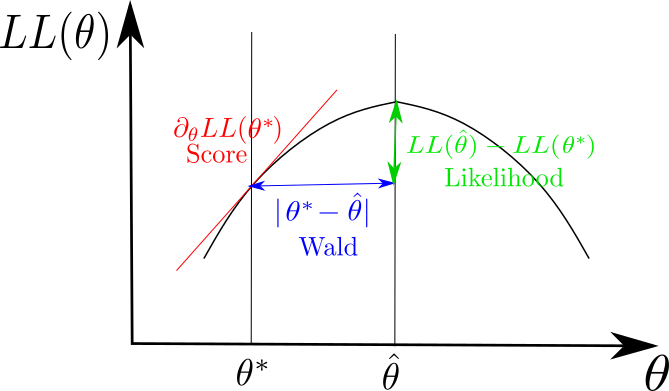
\includegraphics[width=3.2in]{conventions/classic-trio.png}
\caption{For $n=1$ and $\theta\in\RR$,
this figure shows the geometrical significance of
certain
quantities that
characterize the
3 classic test statistics
(Likelihood, Score, Wald)
for hypothesis testing.}
\label{fig-classic-trio}
\end{figure}

Henceforth in this section,
we will
occasionally  use the
Einstein summation
convention; i.e., implicit sum over
repeated indices.

Three classic test statistics
are (See Fig.\ref{fig-classic-trio}):

\begin{enumerate}

\item
{\bf Likelihood Ratio test statistic}
(Ref.\cite{wiki-Li-test}.)

\beq
\lam_{Li}=
2\ln\left[
\frac{L(\HAT{\theta})}
{L(\theta^*)}
\right]=
2[LL(\HAT{\theta})-LL(\theta^*)]
\eeq

\item
{\bf Score (a.k.a.
Lagrange multiplier) test statistic}
(Ref.\cite{wiki-Sc-test}.)

\beqa
\lam_{Sc}&=&
\partial_{\theta_i} LL(\theta^*)
\left[
FI(\theta^*)^{-1}\right]_{i,j}
\partial_{\theta_j} LL(\theta^*)
\\
&=&
\frac{[\partial_\theta LL(\theta^*)]^2}
{FI(\theta^*)}\quad \text{if $n=1$}
\eeqa
Doesn't depend on $\HAT{\theta}$.

\item
{\bf Wald test statistic}
(Ref.\cite{wiki-Wa-test}.)


\beqa
\lam_{Wa}&=&
(\HAT{\theta}-\theta^*)_i
\left[
\av{\HAT{\rvtheta},\HAT{\rvtheta}^T}^{-1}
\right]_{i,j}
(\HAT{\theta}-\theta^*)_j
\label{eq-wald-stat}
\\
&=&
\frac{(\theta^*-\HAT{\theta})^2}
{\av{\HAT{\theta},\HAT{\theta}}}
\quad\text{if $n=1$}
\eeqa

More generally,
one can replace $\theta^*\rarrow R\theta^*$
and  $\HAT{\theta}\rarrow R\HAT{\theta}$
in Eq.(\ref{eq-wald-stat}),
where $\theta^*$ and
$\HAT{\theta}$ are $n$ dimensional
column vectors, and
$R\in\RR^{\nu\times n}$.
The null and alternative hypotheses become:
$H_0: R\theta=R\theta^*$
and $H_1: R\theta\neq R\theta^*$.
Note that
$\nu$
is the number of
constraints imposed by the
null hypothesis. $R$ is called a
reparametrization of $\theta$.
The Wald test is not
reparametrization
invariant (i.e., $R$
invariant), but the Likelihood Ratio test is.

\end{enumerate}

Note that
if $LL(\theta)$
is given by Eq.(\ref{eq-normal-ll}),
then
$\av{\HAT{\rvtheta},\HAT{\rvtheta}}
=
\s^2=\frac{1}{FI(\theta)}
$. Hence,

\beq
\lam_{Li}=\lam_{Sc}=\lam_{Wa}=
\frac{(\HAT{\theta}-\theta^*)^2}{\s^2}
\eeq

Many
other commonly used test statistics
(or their squares)
are special cases of one
of the 3 classic test statistics.
For example, the z-statistic
used with normal
distributions,
the t-statistic
used with the
Student t-distribution,
the F-statistic used in linear regression,
the chi-squared statistic used
to do Pearson's chi-squared test.

{\bf Asymptotic Behavior}

If the data
$\vec{x}$ is i.i.d.,

\beq
P(\vec{x}|\theta)=
\prod_{\s=0}^{nsam-1} P(x^\s|\theta)
\;
\eeq
Hence, as $nsam\rarrow \infty$,

\beqa
LL(\theta)
&=&
\ln P(\vec{x}|\theta)
\\
&=&\sum_\s \ln
P(x^\s|\theta)
\\
&\rarrow&
nsam \sum_x P(x|\theta)\ln  P(x|\theta)
\\
&=&
-nsam \; H(\rvx|\theta)
\eeqa
Thus, {\it maximizing} the log likehood
$LL(\theta)$
and {\it minimizing} the entropy
$H(\rvx|\theta)$
give the same estimate $\HAT{\theta}$.

When the
data is i.i.d. and
$nsam\rarrow \infty$,
it is also possible to
prove that
the 3 test statistics
defined above all tend to
the same
probability  distribution, namely
$\calx^2(\theta^*; \nu)$,
the chi-square distribution
with $\nu$ degrees of freedom,
where $\theta\in \RR^n$, $R\in \RR^
{\nu\times n}$, and $\nu=n$ if $R=1$.

\section{Error Bars}
Never report measurements without error bars!!

Assume a distribution
with mean $\mu$ and
standard deviation $\s$
for a subpopulation with $n$
samples.

$SE=\frac{\s}{\sqrt{n}}$
is called the {\bf standard error}.


Some popular types of error bars:


\begin{itemize}
\item{\bf Box and Whiskers plot (a.k.a. Boxplot)}

See Fig.\ref{fig-boxplot}.
$IQR$ stands for {\bf
Intermediate Quantile Range}.
Sometimes, the endpoints of the
error bars are taken to be the minimum and maximum samples
instead of $Q_1- 1.5 *IQR$ and $Q_3+ 1.5 *IQR$.
The points that fall
in the intervals $[\min,Q_1- 1.5* IQR]$
and $[Q_3+ 1.5 *IQR, \max]$
are
called {\bf outliers}.
\begin{figure}[h!]
\centering
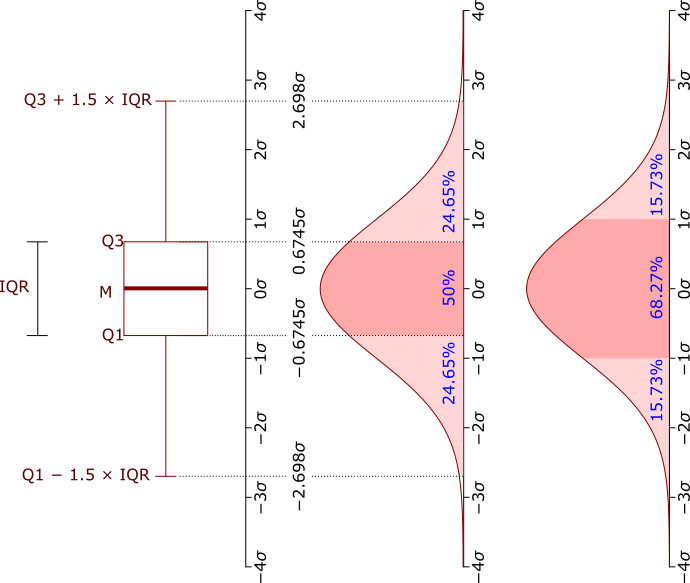
\includegraphics[width=3.3in]
{conventions/Boxplot.png}
\caption{Boxplot plot for Normal
distribution $\caln(\mu=0,\s)$.
$Q_1$ and $Q_3$ are the first and third
quantiles, and $M$ is the median (i.e., half-way point).
For a non-normal skewed
distribution, $Q_1$ and $Q_3$
are not equidistant from the median, and the
median is not exactly equal to the mean. }
 \label{fig-boxplot}
\end{figure}



\item{\bf Standard Deviation}

Error bar endpoints are located one standard deviation
away from the mean.
\beq
\mu-\s< \mu < \mu+\s
\eeq

\item{\bf Confidence Interval}

\beq
\mu-|z^*|SE <\mu < \mu+|z^*|SE
\label{eq-conf-int}
\eeq

$|z^*|=1.96$ for a confidence level of $95\%$.

The origin of Eq.(\ref{eq-conf-int})
is explained in the next section entitled ``Confidence Intervals".
Confidence intervals are
derived from the Gaussian in Fig.\ref{fig-conf-int},
which should not be confused with the
Gaussian of Fig.\ref{fig-boxplot}.
They are different!

\end{itemize}
\section{Confidence Interval}

Normal distribution
with mean $\mu$
and standard deviation $\sigma$:

\beq
\caln(x;\mu, \s^2)=
\frac{1}{\s\sqrt{2\pi}}
e^{-\;\frac{(x-\mu)^2}{2\sigma^2}}
\;.
\eeq

Standard Normal Distribution (SND):
\beq
P(z)=\caln(z;0,1)
\eeq
Cumulative distribution for $P(z)$:

\beq
\Phi(z)=\int_{-\infty}^z dz'\;P(z')
\;.
\eeq

\begin{figure}[h!]
\centering
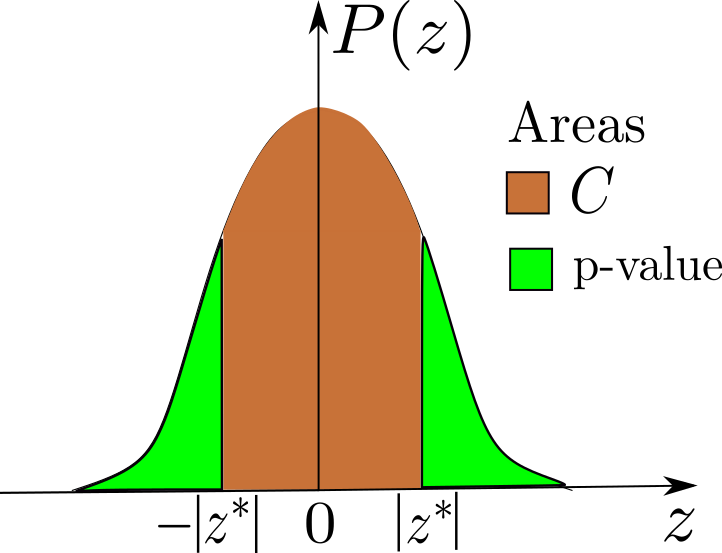
\includegraphics[width=2in]
{conventions/conf-int.png}
\caption{
Interpretation
of confidence level $C$
and p-value as areas under curve of the
Standard Normal Distribution (SND).}
\label{fig-conf-int}
\end{figure}

{\bf Confidence Level} $C$
and corresponding {\bf $|z^*|$ value}
(see Fig.\ref{fig-conf-int}):

\beq
C=\int_{-|z^*|}^{|z^*|} dz\;P(z) =
\Phi(|z^*|)-\Phi(-|z^*|)
=
2\left(\Phi(|z^*|)-\;\frac{1}{2}\right)
\label{eq-conf-level1}
\eeq
Equivalent definition:

\beq
C=P\left(
\underbrace{
\frac{|\rvx-\mu|}{\frac{\sigma}{\sqrt{n}}}
}_{|\rvz|}
<|z^*|\right)
\label{eq-conf-level2}
\eeq
For $C=95\%$,
$|z^*|=1.960\approx 2$.
For $C=99\%$, $|z^*|=2.576$.

Area of each tail
in Fig.\ref{fig-conf-int} is
usually called $\alpha$,
and the area of both tails is called
the {\bf p-value}:
\beq
C+\underbrace{2\alpha}_{p-value}=1
\;.
\eeq

Estimators\footnote{Don't
confuse the sample index $\s$
with the standard deviation $\s$.} of
mean $\mu$  and
standard deviation $\sigma$
from measurements $x^\s$
of a sub-population $\Sigma_1$ of
size $n=|\Sigma_1|$:
\beq
\HAT{\mu}=\ol{x}=\frac{1}{n}\sum_{\s \in\Sigma_1} x^\s
\eeq

\beq
\HAT{\s}^2=
\frac{1}{n-1}
\sum_{\s\in \Sigma_1} (x^\s-\ol{x})^2
\eeq


We get
from Eq.(\ref{eq-conf-level2}),
the {\bf Error bars (a.k.a. confidence intervals)}
and
{\bf Error $E$ (a.k.a. margin of error)}:



\beq
\text{ estimate of $x$
with error bars} =
\ol{x} \pm
\underbrace{
|z^*| \frac{\HAT{\s}}{\sqrt{n}}}_{E}
\label{eq-err-bars}
\eeq

\beq
n= \left(
\frac{|z^*|\HAT{\s}}{E}
\right)^2
\eeq

So far, we have assumed
that the sub-population (a.k.a. sample
population)
is normally distributed.
This might be false
for several reasons.
Some red flags: (1)
$n$ is too small (according to
a rule of thumb derived from
Central Limit Theorem, $n$
should be larger than 30
to insure a Normal Distribution).
(2) Sub-population not truly random
(i.i.d.)
because was taken
without replacement.
In many cases,
especially
when $n<30$,
the Student's t-distribution
models the sub-population statistics
much
better than the Normal distribution.


The {\rm Student's t-distribution } ${\rm Stud}(t;
\nu=n-1)$,
depends
on a parameter $\nu$
called the
number of
degrees of freedom.
In the case being considered here,
$\nu$ equals the
sub-population size $n$
minus one.
When fitting
the data with
Stud(), variable
$t$ replaces
variable $z$,
and ${\rm Stud}(t; \nu=n-1)$
replaces the Standard Normal distribution (SND)
$\caln(z; \mu=0, \sigma=1)$.
Stud() is symmetric about
the origin like SND,
but its tails
are fatter.
When fitting the data with Stud(),
the $|z^*|$
value is replaced
by a $|t^*|$ value.
Eq.(\ref{eq-conf-level1})
is replaced by


\beq
C=\int_{-|t^*|}^{|t^*|} dt\;{\rm Stud}(t) =
\Phi_S(|t^*|)-\Phi_S(-|t^*|)
=
2\left(\Phi_S(|t^*|)-\;\frac{1}{2}\right)
\label{eq-conf-level1-stu}
\;,
\eeq
where $\Phi_S()$
is the cumulative
distribution for  Stud().
Also, Eq.(\ref{eq-err-bars})
is replaced  by

\beq
\text{estimate of $x$
with error bars} =
\ol{x} \pm
\underbrace{
|t^*| \frac{\HAT{\s}}{\sqrt{n}}}_{E}
\;.
\eeq
Tables of $|t^*|(C,\nu=n-1)$
are available. Note
that $|t^*|$
depends on both $C$ and $\nu$,
whereas $|z^*|(C)$
depends only on $C$.

\section{p-value}


Given a parameter $\theta$, call
$\theta=\theta_0$ (or  $\theta<\theta_0$ or $\theta>\theta_0$) the
{\bf null hypothesis} $h_0$,
and call the negation of $h_0$ (i.e., 
$\theta\neq\theta_0$ (or  $\theta\geq\theta_0$ or $\theta\leq \theta_0$))
the {\bf alternative hypothesis} $h_1$.
Assume we
are given data $\vec{x}=\{x^\s|\s\in \Sigma\}$. Assume
also that we are given
distributions $P(\rvx=x|h)$ for $h\in \{h_0, h_1\}$,
and $P(\rvx=x)$. Now let

\beq
P(\vec{x}|h)=\prod_\s P(\rvx=x^\s|h)
\eeq


\beq
P(\vec{x})=\prod_\s P(\rvx=x^\s)
\eeq
(so the $x^\s$ are i.i.d.).

A Bayesian would assume that there
is a prior $P(h)$, and use it to
calculate
$P(h|\vec{x})=\frac{P(\vec{x}|h) P(h)}{P(\vec{x})}$.
$P(\rvh= h_0|\vec{x})$
is the probability that the null hypothesis is true.
A p-value is a monotonically increasing function of
$P(\rvh= h_0|\vec{x})$,
so Bayesians have no trouble saying
that  {\color{red} a p-value is
a measure of
$P(\rvh= h_0|\vec{x})$, i.e.,
a measure of the probability that
the null-hypothesis is true}.

Frequentists, on the other hand,
believe that $h$
is a ``parameter", not a random variable,
so  $P(\rvh= h_0|\vec{x})$
is undefined.
Next, we explain the correct
way of thinking about p-values, according to
Frequentists.
p-values were invented by Frequentists,
so it's worth hearing what they have to say
about them.
The Frequentist definition is not against Bayesianism,
and Bayesians, unlike Frequentists,
 don't accuse Frequentists of
having a sinfully incorrect
 definition of p-values. A Bayesian would just say:
our definition of p-values (shown
in red above) is not incorrect,
but the Frequentist definition is more precise than ours,
and doesn't assume a particular form for a prior.
We welcome it.

Call
the random variable
$\rvt$ the {\bf test statistic} and let 
$t^*$ be a user defined
parameter.
$\rvt$ and $t^*$
are defined so that
when $\rvt=t^*$,
the $h_0$ hypothesis is
on the threshold between 
being and not being satisfied.
Frequentists define the {\bf p-value} $p$ as

\beq
p=
\left\{
\begin{array}{ll}
P(\rvt \geq t^*|h_0)&\text{right-sided-tail,
if $h_0$ is $\theta<\theta_0$}
 \\
 P(\rvt\leq t^*|h_0)&\text{left-sided-tail,
 if $h_0$ is $\theta>\theta_0$}
 \\
 P(|\rvt| > |t^*|\;|h_0)&\text{double-sided-tail,
 if $h_0$ is $\theta=\theta_0$}
\end{array}
\right.
\eeq
Thus, for a Frequentist,
{\color{red} a p-value is a probabilistic
weight of the region
where the $h_0$ hypothesis is
defined (by the user) to be violated}.
If that weight is large,
then the region where
the $h_0$ hypothesis is
defined to be satisfied is small,
which means the $h_0$
hypothesis
is expected to be close to the truth.
The larger the p-value,
the closer $h_0$
is expected to be near the truth,
just like the Bayesian definition
says.
Note that the p-value
is a probability so it ranges in
value from 0 to 1.

Suppose we are given a subpopulation with $n$ samples,
 mean $\ol{x}$ and variance $\HAT{\s}$.
 Let $\theta_0=\mu_0$.
Define

\beq
\rvt=\rvz=
\frac{\rvx-\mu_0}{\frac{\HAT{\s}}{\sqrt{n}}}
\;. 
\eeq
For $n>30$, 

\begin{subequations}
\beqa
P(\rvz\geq z^*|h_0)
=1-\Phi(z^*)=\Phi(-z^*)
&\quad&\text{if $h_0$ is $\mu<\mu_0$}
\\
P(\rvz\leq z^*|h_0)=\Phi(z^*)
&\quad&\text{if $h_0$ is $\mu>\mu_0$}
\\
P(|\rvz|\geq |z^*|\;|h_0)=2\Phi(-|z^*|)
&\quad&\text{if $h_0$ is $\mu=\mu_0$}
\label{eq-double-tail}
\eeqa
\end{subequations}
where $\Phi(x)$ is the cumulative distribution
for the Standard Normal Distribution
$\caln(x;\mu=0, \s=0)$.
For $n<30$, $\Phi()$ is replaced
by $\Phi_S()$, where  $\Phi_S()$ is
the cumulative distribution
for the Student t-distribution ${\rm Stud}(x; \nu=n-1)$.
Note that Eq.(\ref{eq-double-tail})
agrees with
Eq.(\ref{eq-conf-level2}).

The quantity
\beq
z_{score}=
\frac{\ol{x}-\mu_0}{\frac{\HAT{\s}}{\sqrt{n}}}
\eeq
is called the {\bf z score}.
If $|z_{score}| > |z^*|$,
then the $h_0$ hypothesis
is defined to be violated
(for the double sided case).

\section{Short Summary of
Boolean Algebra}
See Ref.\cite{wiki-bool} for more info
about this topic.

Suppose $x, y, z\in \bool$. Define

\beq
x\text{ or }y=x\V y= x+y-xy
\;,
\eeq

\beq
x \text{ and }y=x\A y= xy
\;,
\eeq
and

\beq
\text{not }x=\ol{x}=1-x
\;,
\eeq
where we are using
normal addition and multiplication
on the right hand sides.\footnote{Note the
difference between $\V$ and modulus
2 addition $\oplus$.
For $\oplus$ (a.k.a. XOR): $x\oplus y=x+y-2xy$.}



\begin{table}[h!]
\centering
\begin{tabular}{|
>{\columncolor[HTML]{ECF4FF}}l |l|}
\hline
Associativity & \begin{tabular}[c]{@{}l@{}}$x \V (y \V z)=(x \V y) \V z$\\ $x \A (y \A z)=(x \A y) \A z$\end{tabular} \\ \hline
Commutativity & \begin{tabular}[c]{@{}l@{}}$x \V y=y \V x$\\ $x \A y=y \A x$\end{tabular} \\ \hline
Distributivity & \begin{tabular}[c]{@{}l@{}}$x \A (y \V z)=(x \A y) \V (x \A z)$\\ $x \V (y \A z)=(x \V y) \A (x \V z)$\end{tabular} \\ \hline
Identity & \begin{tabular}[c]{@{}l@{}}$x \V 0=x$\\ $x \A 1=x$\end{tabular} \\ \hline
Annihilator & \begin{tabular}[c]{@{}l@{}}$x \A 0=0$\\ $x \V 1= 1$\end{tabular} \\ \hline
Idempotence & \begin{tabular}[c]{@{}l@{}}$x \V x= x$\\ $x \A x= x$\end{tabular} \\ \hline
Absorption & \begin{tabular}[c]{@{}l@{}}$x \A (x \V y)= x$\\ $x \V (x \A y)= x$\end{tabular} \\ \hline
Complementation & \begin{tabular}[c]{@{}l@{}}$x \A \ol{x} = 0$\\ $x \V \ol{x}   = 1$\end{tabular} \\ \hline
Double negation & $\ol{(\ol{x})} = x$ \\ \hline
De Morgan Laws & \begin{tabular}[c]{@{}l@{}}$\ol{x} \A \ol{y} =\ol{(x \V y)}$\\ $\ol{x} \V \ol{y} = \ol{(x \A y)}$\end{tabular} \\ \hline
\end{tabular}
\caption{Boolean Algebra Identities}
\label{tab-bool-alg}
\end{table}

Actually, since
$x\A y=xy$, we can omit writing
the symbol $\A$. The symbol
$\A$ is useful to
exhibit the symmetry
of the identities, and
to remark
about
the analogous identities
for sets, where
$\A$ becomes intersection $\cap$
and $\V$ becomes union $\cup$. However,
for practical calculations,
$\A$ is an unnecessary nuisance.

Since $x\in \bool$,
\beq
P(\ol{x})=1-P(x)
\;.
\eeq

Clearly, from analyzing
the simple event space $(x,y)\in \bool^2$,
\beq
P(x\V y)= P(x) + P(y) - P(x\A y)
\;.
\eeq

\chapter{Basic Curve Fitting
Using Gradient Descent}
\label{ch-basic-fit}

\begin{figure}[h!]
\centering
$$\xymatrix{
&\vec{\rvx}\ar[d]\ar[r]&\ul{\vecy}
\ar[d]&\\
\phi\ar[r]\ar@/_1pc/[rrr]&
\vec{\hat{\rvy}}\ar[r]&\cale\ar[r]&\phi'
}$$
\caption{Basic curve fitting bnet.}
\label{fig-bfit}
\end{figure}


Samples 
$(x[i], y[i])\in S_\rvx\times S_\rvy$
are given. $nsam(\vecx)=nsam(\vecy)$.

Estimator function 
$\hat{y}(x; \phi)$
for $x\in S_\rvx$ and $\phi\in\RR$
is given.

Let 
\beq
P_{\rvx, \rvy}(x,y)=
\frac{1}{nsam(\vecx)}
\sum_i \indi(x=x[i], y=y[i])
\;.
\eeq


Let 
\beq
\cale(\vecx, \vecy, \phi)=
\frac{1}{nsam(\vec{y})}
\sum_i
|y[i]-\hat{y}(x[i]; \phi)|^2
\;
\eeq
$\cale$ is called the mean square error.

Best fit is parameters $\phi^*$
such that

\beq 
\phi^*= \argmin_\phi
\cale(\vecx, \vecy, \phi)
\;.
\eeq

The node TPMs for
the basic curve fitting bnet
 Fig.\ref{fig-bfit} are
printed below in blue.

\beq\color{blue}
P(\phi) \text{ = given}
\;.
\eeq
The first time
it is used, $\phi$ is arbitrary.
After the first time, it is determined 
by previous stage.

\beq\color{blue}
P(\vecx)=\prod_i P_\rvx(x[i])
\eeq

\beq\color{blue}
P(\vecy|\vecx)=\prod_i P_{\rvy|\rvx}(y[i]\cond x[i])
\eeq

\beq\color{blue}
P(\hat{y}[i]|\phi, \vecx)=
\delta(\hat{y}[i], \hat{y}(x[i];\phi))
\eeq


\beq\color{blue}
P(\cale|\vec{\hat{y}}, \vecy)=
\delta(\cale,\frac{1}{nsam(\vecx)}
\sum_i |y[i]-\hat{y}[i]|^2)
\;.
\eeq


\beq\color{blue}
P(\phi'|\phi, \cale)=
\delta(\phi',
\phi-\eta\partial_\phi\cale)
\eeq
$\eta>0$ is the descent rate.
If $\Delta \phi=\phi'-\phi=-\eta 
\frac{\partial\cale}
{\partial \phi}$, then
 $\Delta \cale=\frac{-1}{\eta}
(\Delta\phi)^2<0$  so this will
minimize the error
$\cale$.
This is called ``gradient descent".
\chapter{Bell  
and Clauser-Horne Inequalities 
in Quantum Mechanics}

\begin{figure}[h!]
\centering
$$\xymatrix{
&\ul{\lambda}\ar[dr]\ar[dl]&\\
\ul{x_1^{\alpha_1}}&&\ul{x_2^{\alpha_2}}
}$$
\caption{bnet used to discuss Bell 
and Clauser-Horne inequalities 
in Quantum Mechanics.}
\label{fig-bell}
\end{figure}

I wrote an article about
this in 2008 for
my blog \qt{Quantum Bayesian Networks}.
See Ref.\cite{bell-blog}.
\chapter{Generative Adversarial Networks
 (GANs)}
%\begin{refsection}

\begin{figure}[h!]
\centering
\includegraphics[width=6in]{gan/gan.png}
\caption{Generative Adversarial  Network (GAN)} 
\label{fig-gan}
\end{figure}

\begin{figure}[h!]
\centering
\includegraphics[width=6in]{gan/gan-detail.png}
\caption{Discriminator node $\ul{V}$ in Fig.\ref{fig-gan} can be
split into 3 nodes $\vec{\rvc}$, $\vec{\rvd}$ and $\ul{V}$.} 
\label{fig-gan-detail}
\end{figure}

Original GAN, 
Ref.\cite{gf2014}(2014). 

Generator $G$ (counterfeiter) generates samples $\vecf$ of fake money and submits them to Discriminator $D$ (Treasury agent). $D$ also gets samples $\vecr$ of real money. $D$ submits veredict $V\in [0,1]$. $G$ depends on parameter $\theta_G$ and $D$ on parameter $\theta_D$. Veredict $V$ and initial $\theta_G, \theta_D$ are used to get new parameters $\theta'_G, \theta'_D$.Process is repeated (Dynamical Bayesian Network) until saddle point in $V(\theta_G, \theta_D)$ is reached. $D$ makes $G$ better and vice versa.  Zero-sum game between $D$ and $G$.



Let $\cald$ be the domain of $D(\cdot, \theta_D)$. Assume that for any $x\in \cald$,

\beq
0\leq D(x,\theta_D)\leq 1
\;.
\eeq
For any $S\subset\cald$, define

\beq
\sum_{x\in S}D(x,\theta_D)=\lam(S,\theta_D)
\;.
\eeq


 In general, 
$G(\cdot,\theta_G)$ need not be real valued. 

Assume that for every $u\in S_\rvu$,
 $G(u,\theta_G)=f\in S_\rvf\subset \cald$. Define
\beq
\ol{D}(f,\theta_D)=1-D(f,\theta_D)
\;.
\eeq
Note that

\beq
0\leq\ol{D}(f,\theta_D)\leq 1
\;.
\eeq

Define:

\beq
V(\theta_G, \theta_D) =
\sum_{r}P(r)
\ln D(r, \theta_D)
+ \sum_{u}P(u)\ln
\ol{D}(G(u,\theta_G),\theta_D)
\;.	
\eeq

We want the first variation of $V(\theta_G, \theta_D)$ to vanish.




\beq
\delta V(\theta_G, \theta_D)=0
\;.
\eeq
This implies

\beq
 \partial_{\theta_G}V(\theta_G, \theta_D)=
 \partial_{\theta_D}V(\theta_G, \theta_D)=0
\;
\eeq
and

\beq
V_{opt}=\min_{\theta_G}\max_{\theta_D} V(\theta_G, \theta_D)
\;.
\eeq

Node TPMs
for Figs.\ref{fig-gan} and \ref{fig-gan-detail} 
are
given next in blue:

\beq\color{blue}
P(\theta_G)=\;{\rm given}
\eeq

\beq\color{blue}
P(\theta_D)=\;{\rm given}
\eeq


\beq\color{blue}
P(\vecu)=\prod_i P(u[i])  \;\;{\rm (usually \;uniform\; distribution)}
\eeq

\beq\color{blue}
P(\vecr)=\prod_i P(r[i])
\eeq


\beq\color{blue}
P(f[i]\cond \vecu, \theta_G)= \delta[f[i], G(u[i],\theta_G)]
\eeq

\beq\color{blue}
P(c[i]\cond \vecf, \theta_D) = \delta(c[i], \ol{D}(f[i], \theta_D))
\eeq

\beq\color{blue}
P(d[j]\cond \vecr, \theta_D)= \delta(d[j], D(r[j], \theta_D))
\eeq




\beq\color{blue}
P(V| \vecd,  \vecc)=
\delta(V, \frac{1}{N}\ln \prod_{i,j}(c[i]d[j]))
\eeq
where $N=nsam(\vecr)nsam(\vecu)$.


Let $\eta_G, \eta_D> 0$. Maximize $V$ wrt $\theta_D$, and
minimize it wrt $\theta_G$.

\beq\color{blue}
P(\theta'_G|V,\theta_G )=
\delta(\theta'_G, \theta_G - \eta_G 
\partial_{\theta_G}V)
\eeq

\beq\color{blue}
P(\theta'_D|V,\theta_D )=
\delta(\theta'_D, \theta_D + \eta_D 
\partial_{\theta_D}V)
\eeq

\hrule
\begin{figure}[h!]
\centering
\includegraphics[width=2in]{gan/gan-emulate.png}
\caption{GAN, Constraining Bayesian Network}
\label{fig-gan-emulate} 
\end{figure}

Constraining B net given in Fig.\ref{fig-gan-emulate}. It adds 2 new nodes, namely $\ul{\vec{U}}$ and $\ul{\vec{R}}$, to  the bnet of Fig.\ref{fig-gan}. The purpose of these 2  barren (childrenless) nodes is to constrain certain functions to be probability distributions.

Node TPMs for the 2 new nodes given next in blue.


\beq\color{blue}
P(U[i]\cond \theta_G)= 
\frac{\ol{D}(G(U[i],\theta_G),\theta_D))}
{\ol{\lam}(\theta_G, \theta_D)}
\eeq
where  $S_{\ul{U[i]}}=S_\rvu$ and $\ol{\lam}(\theta_G, \theta_D)=\sum_u\ol{D}(G(u, \theta_G), \theta_D))$.

\beq\color{blue}
P(R[i]\cond \theta_G, \theta_D)= \frac{D(R[i], \theta_D)}{\lam(\theta_D)}
\eeq
where $S_{\ul{R[i]}}=S_\rvr$ and  $\lam(\theta_D)=\sum_r D(r, \theta_D)$.


\beq\color{blue}
P(V| \vecu,  \vecr)=
\delta(V, \frac{1}{N}\ln \prod_{i,j}(
P(\ul{R[i]}=r[i]\cond \theta_G, \theta_D)P(\ul{U[i]}=u[j]\cond \theta_G)))
\eeq
where $N=nsam(\vecr)nsam(\vecu)$.


$\call=$ likelihood
\beqa
\call&=&
P(\vecr, \vecu| \theta_G, \theta_D)\\
&=&
\prod_{i,j}\left[
 \frac{D(r[i], \theta_D)}{\lam(\theta_D)}
\frac{\ol{D}(G(u[j],\theta_G),\theta_D))}
{\ol{\lam}(\theta_G, \theta_D)}
\right]
\eeqa

\beq
\ln \call = N[V(\theta_G, \theta_D)
-\ln \lam(\theta_D)-\ln \ol{\lam}(\theta_G, \theta_D)]
\eeq



%\printbibliography[heading=subbibliography]
%\end{refsection}


 
%
\chapter{IN PROGRESS: Generative Adversarial Networks, Ensemble GANs}
\begin{refsection}
Bayesian GAN, 
 Ref.\cite{wilson2017} (2017)

Replace $\theta_a$ by $\vtheta_a$ and 
$\theta'_a$ by $\vtheta'_a$ for $a=G,D$



\beq
\delta V(\vtheta_G, \vtheta_D)=0
\eeq

\beq
 \partial_{\vtheta_G}V(\vtheta_G, \vtheta_D)=
 \partial_{\vtheta_D}V(\vtheta_G, \vtheta_D)=0
\eeq

\beq
V_{opt}=\min_{\vtheta_G}\max_{\vtheta_D} V(\vtheta_G, \vtheta_D)
\eeq

\beq
P(\vtheta_G)=\prod_i P(\theta_G[i])
\eeq

\beq
P(\vtheta_D)=\prod_i P(\theta_D[i])
\eeq


\beq
P(\vecu)=\prod_i P(u[i])
\eeq

\beq
P(\vecr)=\prod_i P(r[i])
\eeq


\beq
P(f[i]|\vecu, \vtheta_G)= \prod_i\delta[f[i], G(u[i],\vtheta_G)]
\eeq

\beq
P(c[i]|\vecf, \vtheta_D) = \delta(c[i], \ol{D}(f[i], \vtheta_D))
\eeq

\beq
P(d[j]|\vecr, \vtheta_D)= \delta(d[j], D(r[j], \vtheta_D))
\eeq


\beq
P(V| \vecd,  \vecc)=
\delta(V, \frac{1}{N}\ln \prod_{i,j}(c[i]d[j]))
\eeq
where $N=nsam(\rvr)nsam(\rvu)$







$\eta_G, \eta_D> 0$, maximize wrt $\theta_D$, 
minimize wrt $\theta_G$
\beq
P(\theta'_G|V,\vtheta_G )=
\delta(\vtheta'_G, \vtheta_G - \eta_G 
\partial_{\vtheta_G}V)
\eeq

\beq
P(\theta'_D|V,\vtheta_D )=
\delta(\vtheta'_D, \vtheta_D + \eta_D 
\partial_{\vtheta_D}V)
\eeq


\hrule
Emulated B net

\beq
P(\vtheta_G)=\;\prod_i P(\theta_G[i])
\eeq

\beq
P(\vtheta_D)=\;\prod_i P(\theta_D[i])
\eeq


\beq
P(u[i]|\vtheta_G, \vtheta_D)=  
\ol{D}(G(u[i],\vtheta_G), \vtheta_D)
\eeq


\beq
P(r[i]|\vtheta_D)=  
D(r[i], \vtheta_D)
\eeq

\beq
P(V| \vecd,  \vecc)=
\delta(V, \prod_{i,j,a,b}(u[i]r[j]\theta_G[a]\theta_D[b]))
\eeq



$\eta_G, \eta_D > 0$, maximize wrt $\theta_D$, 
minimize wrt $\theta_G$
\beq
P(\vtheta'_G|V,\vtheta_G )=
\prod_i \delta(\theta'_G[i], \theta_G[i] - \eta_G 
\partial_{\theta_G[i]}\ln V)
\eeq

\beq
P(\vtheta'_D|V,\vtheta_D )=\prod_i
\delta(\theta'_D[i], \theta_D[i] + \eta_D 
\partial_{\theta_D[i]}\ln V)
\eeq

\beq
P(\vecr, \vecu, \vtheta_G, \vtheta_D)=
\prod_{i,j,a,b}
\left\{
P(\theta_G[a])P(\theta_D[b])\\
 \frac{D(r[i], \theta_D[b])}{\lam(\theta_D[b])}
\frac{\ol{D}(G(u[j],\theta_G[a]),\theta_D[b]))}
{\ol{\lam}(\theta_G[a], \theta_D[b])}
\right\}
\eeq


$N=nsam(\vecr)nsam(\vecu)
nsam(\vtheta_G)nsam(\vtheta_D)$

\beq
\ln P(\vecr, \vecu, \vtheta_G, \vtheta_D) =
N\left\{
\begin{array}{l}
-H(P_{\ul{\theta}_D})+ \sum_{r,\theta_D}P(r)P(\theta_D)
\ln \frac{D(r, \theta_D)}{\lam(\theta_D)}
\\
-H(P_{\ul{\theta}_G})+ \sum_{u,\theta_G,\theta_D}P(u)
P(\theta_G)P(\theta_D)\ln
\frac{\ol{D}(G(u,\theta_G),\theta_D)}{\ol{\lam}(\theta_G, \theta_D)}
\end{array}
\right.
\eeq

\beq
\ln P(\vecr, \vecu) =
N\left\{
\begin{array}{l}
 \sum_{r}P(r)
\ln \sum_{\theta_D}P(\theta_D)\frac{D(r, \theta_D)}{\lam(\theta_D)}
\\
+ \sum_{u}P(u)
\ln \sum_{\theta_D, \theta_G}
P(\theta_G)P(\theta_D)
\frac{\ol{D}(G(u,\theta_G),\theta_D)}{\ol{\lam}(\theta_G, \theta_D)}
\end{array}
\right.
\eeq

\beqa
V(\vtheta_G, \vtheta_D) &=&\frac{1}{N} \ln P(\vtheta_G, \vtheta_D|\vecr,\vecu,)\\&=&
\frac{1}{N} [
\ln P(\vecr,\vecu,\vtheta_G, \vtheta_D)
-\ln P(\vecr,\vecu)]
\eeqa



\printbibliography[heading=subbibliography]
\end{refsection}

\chapter{Kalman Filter}\label{ch-kalman}

A Kalman Filter is a special case of a
Hidden Markov Model. HMMs are
 discussed in Chapter \ref{ch-hmm}.

\begin{figure}[h!]
\centering
$$\xymatrix{
\rvx_0\ar[d]\ar[r]&
\rvx_1\ar[d]\ar[r]&
\rvx_2\ar[d]\ar[r]&
\rvx_3\ar[d]\\
\rvz_0&
\rvz_1&
\rvz_2&
\rvz_3
}$$
\caption{Kalman Filter bnet with $T=4$.}
\label{fig-kal}
\end{figure}

Let $t=0, 1, 2, \dots , T-1$.

$\rvx_t\in S_\rvx$ are
random variables that represent
the hidden (unobserved) true
state of the system.

$\rvz_t\in S_\rvz$ are 
random variables that represent
the measured (observed) state of the system.


The Kalman Filter bnet Fig.\ref{fig-kal}
has the following
node TPMs,
printed in blue:


\beq\color{blue}
P(x_t|x_{t-1})=
\caln(x_t;F_tx_{t-1} + B_tu_t, Q_t)\;,
\eeq
where $F_t, Q_t, B_t, u_t$
are given. $P(x_t|x_{t-1})$ becomes $P(x_t)$
for $t=0$.

\beq\color{blue}
P(z_t|x_t)=
\caln(z_t; H_tx_t, R_t)
\;,
\eeq
where $H_t, R_t$ are given.

Define

\beq
\rvZ_t= (\rvz_{t'})_{t'\leq t}
\;.
\eeq
Define $\hat{x}_t$ and $P_t$ by

\beq
P(x_t|Z_t)=
\caln(x_t; \hat{x}_t, P_t)
\;.
\eeq
\hrule
\medskip
\noindent
Problem: Find $\hat{x}_t$ and $P_t$
in terms of 
\begin{enumerate}
\item
 current (at time $t$)
 given values of
$F,Q,H,R,
 B ,u$
\item
 current (at time $t$)
observed  value of 
$z$
\item
prior (previous)
value (at time $t-1$) of $\hat{x}$
and $P$.
\end{enumerate}
See Fig.\ref{fig-kal-plus}.
For that figure,

\beq \color{blue}
P(\hat{x}_t, P_t | z_t,
\hat{x}_{t-1}, P_{t-1})
=\delta(\hat{x}_t,?)
\delta(P_t, ?)
\;.
\eeq

\begin{figure}[h!]
\centering
$$\xymatrix{
\rvx_0\ar[d]\ar[r]&
\rvx_1\ar[d]\ar[r]&
\rvx_2\ar[d]\ar[r]&
\rvx_3\\
\rvz_0\ar[d]&
\rvz_1\ar[d]&
\rvz_2\ar[d]&
\rvz_3\\
\ul{\hat{x}}_0, 
\ul{P}_0\ar[r]&
\ul{\hat{x}}_1, 
\ul{P}_1\ar[r]&
\ul{\hat{x}}_2, 
\ul{P}_2\ar[r]&
\ul{\hat{x}}_3, 
\ul{P}_3
}$$
\caption{Kalman Filter bnet
with deterministic nodes for 
$\hat{x}_t, P_t$.}
\label{fig-kal-plus}
\end{figure}

\hrule \noindent
Solution copied from Wikipedia Ref.\cite{wiki-kalman}:


Define $\eta_{t|t}=\eta_t$ for 
$\eta=\hat{x}, P$.

\begin{itemize}
\item{\bf Predict}

Predicted (a priori) state estimate
\beq
\hat{\mymathbf{x}}_{t\mid t-1} =
 \mymathbf{F}_t
\hat{\mymathbf{x}}_{t-1\mid t-1}
 + \mymathbf{B}_t \mymathbf{u}_{t}
\eeq

Predicted (a priori) estimate covariance
\beq
\mymathbf{P}_{t\mid t-1} =
 \mymathbf{F}_t 
\mymathbf{P}_{t-1\mid t-1}
 \mymathbf{F}_t^\textsf{T} +
 \mymathbf{Q}_t
\eeq

\item{\bf Update}

Innovation (or measurement 
pre-fit residual)
\beq
\tilde{\mymathbf{y}}_{t|t-1}= 
\mymathbf{z}_t - 
\mymathbf{H}_t\hat{\mymathbf{x}}_{t\mid t-1}
\eeq

Innovation (or pre-fit residual)
 covariance
\beq
\mymathbf{S}_t = \mymathbf{H}_t 
\mymathbf{P}_{t\mid t-1} 
\mymathbf{H}_t^\textsf{T} +
 \mymathbf{R}_t
\eeq

\end{itemize}


Optimal Kalman gain
\beq
\mymathbf{K}_t = \mymathbf{P}_{t\mid t-1}
\mymathbf{H}_t^\textsf{T}
 \mymathbf{S}_t^{-1}
\eeq


Updated (a posteriori) state estimate
\beq
\hat{\mymathbf{x}}_{t\mid t} =
 \hat{\mymathbf{x}}_{t\mid t-1} +
 \mymathbf{K}_t\tilde{\mymathbf{y}}_t
\eeq

Updated (a posteriori) estimate covariance
\beq
\mymathbf{P}_{t|t} = \left(\mymathbf{I} -
 \mymathbf{K}_t \mymathbf{H}_t\right) 
\mymathbf{P}_{t|t-1} 
\eeq

Measurement post-fit residual
\beq
\tilde{\mymathbf{y}}_{t\mid t} =
 \mymathbf{z}_t - \mymathbf{H}_t
\hat{\mymathbf{x}}_{t\mid t}
\eeq
\chapter{Linear and Logistic Regression}
%\begin{refsection}

\begin{figure}[h!]
\centering
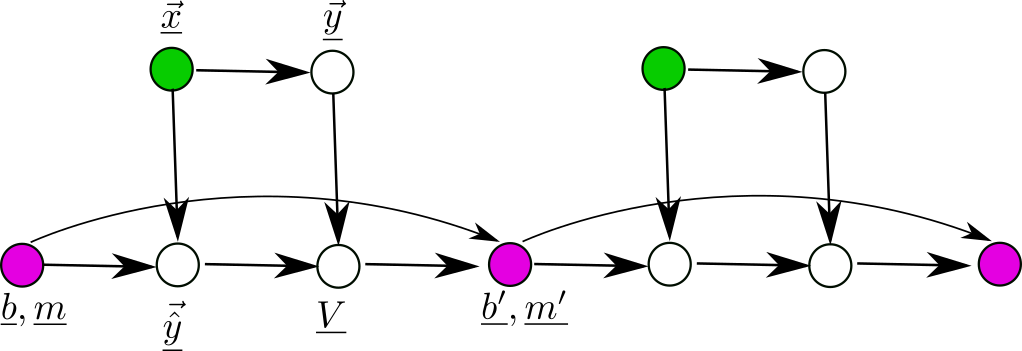
\includegraphics[width=5in]{linreg/linreg.png}
\caption{Linear Regression}
\label{fig-linreg}
\end{figure}

\begin{figure}[h!]
\centering
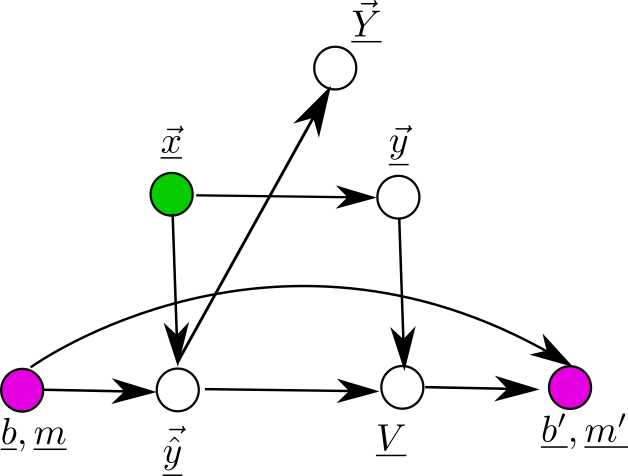
\includegraphics[width=3in]{linreg/linreg-emul.png}
\caption{Bnet of Fig.\ref{fig-linreg}  with new $\vec{\ul{Y}}$ node.}\label{fig-linreg-emul}
\end{figure}



Estimators $\haty$ for linear and logistic regression.
\begin{itemize}
\item

\textbf{Linear Regression:} $y\in \RR$.
Note $\haty\in \RR$. $(x,\haty(x))$ is
the graph
of a straight line
with y-intercept $b$ and slope $m$.
\beq
\haty(x;b, m)= b + mx
\eeq

\item
\textbf{Logistic Regression:} $y\in\{0, 1\}$. Note $\haty\in [0,1]$. $
(x,\haty(x))$ is the graph
of a sigmoid.
 Often in literature, $b,m$ are replaced by $\beta_0, \beta_1$.
\beq
\haty(x;b, m)=\smoid(b + m x)
\eeq
\end{itemize}

Define
\beq
V(b, m)=\sum_{x,y}P(x,y)| y-\haty(x;b, m)|^2
\;.\label{eq-norm-cost}
\eeq
We want to minimize $V(b,m)$ (called a cost or loss function) wrt $b$ and $m$.


The TPMs, printed in blue, for the
Bnet Fig.\ref{fig-linreg}, are as follows.

\beq\color{blue}
P(b,m) \text{ = given}
\eeq
The first time it is used,
$(b,m)$ is arbitrary.
After the first time, it is determined
by previous stage.

Let
\beq
P_{\rvx, \rvy}(x,y)=
\frac{1}{nsam(\vecx)}
\sum_\s \indi(x=x^\s, y=y^\s)
\;.
\eeq

\beq\color{blue}
P(\vecx)=\prod_\s P(x^\s)
\eeq

\beq\color{blue}
P(\vecy|\vecx)=\prod_\s P(y^\s\cond x^\s)
\eeq

\beq\color{blue}
P(\vec{\haty}|\vecx, b, m)=\prod_\s \delta(\haty^\s, \haty(x^\s,b,m))
\label{eq-replace1}
\eeq

\beq\color{blue}
P(V|\vec{\haty}, \vecy)=
\delta(V, \frac{1}{nsam(\vecx)}\sum_\s |y^\s-\haty^\s|^2)
\label{eq-replace2}
\eeq
Let $\eta_b, \eta_m>0$.
For $x=b,m$, if
$x'-x=\Delta x =
-\eta\frac{\partial V}{\partial x}$,
 then $\Delta V\approx
 \frac{-1}{\eta}(\Delta x)^2   \leq 0$
 for $\eta>0$. This is called \enquote{gradient descent}.
\beq\color{blue}
P(b'|V, b)=\delta(b', b-\eta_b\partial_b V)
\eeq
\beq\color{blue}
P(m'|V, m)=\delta(m', m-\eta_m\partial_m V)
\eeq


\section{Generalization to
$x$ with multiple
components (features)}

 Suppose that for each sample $\s$,
instead of $x^\s$ being a scalar,
it has $n$ components called features:

 \beq
x^\s = (x_0^\s, x_1^\s, x_2^\s , \ldots x_{n-1}^\s)
\;.\eeq

Slope $m$ is replaced by weights

\beq
w = (w_0, w_1, w_3, , \ldots, w_{n-1})
\;,\eeq
and the product of 2  scalars $mx^\s$ is replaced by the inner vector product $w^Tx^\s$.

\section{Alternative $V(b,m)$
 for logistic regression}

For logistic regression, since $y^\s\in \{0,1\}$
 and $\haty^\s\in [0,1]$ are both
in the interval $[0,1]$, they can
be interpreted as probabilities. Define
probability distributions $p^\s(x)$ and
$\HAT{p}^\s(x)$ for $x\in \{0,1\}$ by
\beq
p^\s(1)=y^\s,\;\;\; p^\s(0)=1-y^\s
\eeq

\beq
\HAT{p}^\s(1)=\haty^\s,\;\;\; \HAT{p}^\s(0)=1-\haty^\s
\eeq
Then for logistic regression, the following 2 cost functions $V(b,m)$
can be used as alternatives to the cost function Eq.(\ref{eq-norm-cost}) previously given.

\beq
V(b, m)= \frac{1}{nsam(\vecx)}\sum_\s
 D_{KL}(p^\s\parallel \HAT{p}^\s)
\eeq

and

\beqa
V(b, m)&=&\frac{1}{nsam(\vecx)} \sum_\s
CE(p^\s\parallel\HAT{p}^\s)\\
&=& \frac{-1}{nsam(\vecx)}\sum_\s \left\{
y^\s\ln \haty^\s +
(1-y^\s)\ln (1- \haty^\s)\right\}\\
&=&
\frac{-1}{nsam(\vecx)}\sum_\s
\ln \left\{(\haty^\s)^{y^\s}
(1- \haty^\s)^{(1-y^\s)}\right\}\\
&=&
\frac{-1}{nsam(\vecx)}\sum_\s
\ln P(\ul{Y}=y^\s\cond \haty=\haty^\s)\\
&=&
-\sum_{x,y} P(x, y)
\ln P(\ul{Y}=y|\haty=\haty(x,b,m))
\eeqa

Above, we used
\beq
P(\ul{Y}=Y|\haty) = \haty^{Y}
[1-\haty]^{1-Y}
\eeq
for $Y\in S_{\ul{Y}}=\{0,1\}$. (Bernoulli distribution).

There is no node corresponding to $\ul{Y}$
in the Bnet of Fig.\ref{fig-linreg}.
Fig.\ref{fig-linreg-emul} shows a new Bnet
that has a new node called $\vec{\ul{Y}}$
compared to the Bnet of Fig.\ref{fig-linreg}.
One defines the TPMs
for all nodes of Fig.\ref{fig-linreg-emul}
except $\vec{\ul{Y}}$ and $\ul{V}$ the same
as for Fig.\ref{fig-linreg}. For $\vec{\ul{Y}}$
and $\ul{V}$, one defines

\beq\color{blue}
P(Y^\s\cond \vec{\haty})=
P(\ul{Y}=Y^\s\cond \haty^\s)
\eeq

\beq\color{blue}
P(V|\vec{Y}, \vecy)=
\delta(V, \frac{-1}{nsam(\vec{x})}\ln  L)
\;,
\eeq
where $ L =\prod_\s P(\ul{Y}=y^\s\cond \haty^\s )$=likelihood.

\chapter{Monty Hall Problem}
\begin{figure}[h!]
\centering
$$\xymatrix{
\rvc\ar[dr]&&\rvy\ar[dl]\\
&\rvm&
}$$
\caption{Monty Hall Problem.}
\label{fig-monty}
\end{figure}

Mr. Monty Hall, host of the 
game show ``Let’s Make a Deal",
 hides a car behind one of 
three doors and a goat 
behind each of the other two.
 The contestant picks Door No. 1,
 but before opening it, Mr. Hall 
opens Door No. 2 to reveal a goat. 
Should the contestant stick with No. 1 
or 
switch to No. 3?

The Monty Hall problem can be 
modeled by the bnet 
Fig.\ref{fig-monty}, where
\begin{itemize}
\item
$\rvc$= the door behind which the car actually is.
\item
$\rvy$= the door opened by you
 (the contestant), on your 
first selection.
\item
$\rvm$= the door opened by Monty (game host)
\end{itemize}

We label the doors 1,2,3 so
 $S_\rvc=S_\rvy=S_\rvm=\{1,2,3\}$.

Node matrices printed in blue:
\beq\color{blue}
P(c)=\frac{1}{3}\text{ for all $c$}
\eeq

\beq\color{blue}
P(y)=\frac{1}{3}\text{ for all $y$}
\eeq

\beq\color{blue}
P(m|c,y)=\hat{1}(m\neq c)\left[
\frac{1}{2}\hat{1}(y=c)
+
\hat{1}(y\neq c)\hat{1}(m\neq y)\right]
\eeq

It's easy to show that the above
 node probabilities imply that
\beq
P(c=1|m=2,y=1)=\frac{1}{3}
\eeq

\beq
P(c=3|m=2,y=1)=\frac{2}{3}
\eeq

So you are twice as likely to
 win if you switch your final
 selection to be the door 
which is neither 
your first choice nor Monty’s choice.

The way I justify this to myself
is: Monty gives you a
 piece of information.
If you don't switch your choice,
you are wasting that info, whereas
if you switch, you are using the info.



\chapter{Naive Bayes}\label{ch-naive}

\begin{figure}[h!]
\centering
$$\xymatrix{
\rvc\ar[d]\ar[dr]\ar[drr]\ar[drrr]\\
\rvx_0&\rvx_1&\rvx_2&\rvx_3
}$$
\caption{bnet for Naive Bayes
with 4 features}
\label{fig-naive}
\end{figure}
Class node $\rvc\in S_\rvc$. $|S_\rvc|=n_\rvc$=
number of classes.

Feature nodes $\rvx_i\in S_{\rvx_i}$ for 
$i=0, 1, 2, \ldots, F-1$. $F$=number of
features.

Define
\beq
x.=[x_0,x_1, \ldots, x_{F-1}]
\;.
\eeq

For the bnet of Fig.\ref{fig-naive},
\beq
P(c, x.)=P(c)
\prod_{i=0}^{F-1}
P(x_i|c)
\;.
\eeq

Given $x.$ values, 
find most likely class $c\in S_\rvc$.

Maximum a Posteriori (MAP) estimate:
\beqa
c^* &=& \argmax_c P(c|x.)\\
&=&\argmax_c \frac{P(c,x.)}{P(x.)}\\
&=&\argmax_c P(c, x.)
\;.
\eeqa

\chapter{Neural Networks}

In this chapter, we discuss
 Neural Networks (NNs) of the
feedforward kind,
which is the most popular kind. In their
 plain, vanilla form, NNs only
have deterministic nodes.
But the nodes of a bnet can
be deterministic too, because
the transition probability matrix
of a node
can reduce to a delta function.
Hence, NNs should be expressible
as bnets. We will confirm this
in this chapter.

Henceforth in this chapter,
if we replace an index of an
indexed quantity by a dot, 
it will mean the collection
of the indexed quantity
for all values of that
index. For example, $x.$
will mean the 
array of $x_i$ for all $i$.


\begin{figure}[h!]
\centering
$$\xymatrix{
\rvx_0\ar@/^1pc/[rr]
\ar@/^2pc/[rrr]
\ar[d]\ar[dr]\ar[drr]\ar[r]&
\rvx_1\ar@/^1pc/[rr]
 \ar[dl]\ar[d]\ar[dr]\ar[r]&
\rvx_2\ar[dll]\ar[dl]\ar[d]\ar[r]&
\rvx_3\ar[dlll]\ar[dll]\ar[dl]\\
\rvh_0^0\ar[d]\ar[dr]&
\rvh_1^0\ar[dl]\ar[d]&
\rvh_2^0\ar[dll]\ar[dl]\\
\rvh_0^1\ar[d]\ar[dr]&
\rvh_1^1\ar[dl]\ar[d]\\
\rvY_0&
\rvY_1
}$$
\caption{Neural Network (feed forward)
with 4 layers: input layer $\rvx.$,
2 hidden layers $\rvh^0.$,
$\rvh^1.$ and
output layer $\rvY.$ }
\label{fig-nn}
\end{figure}

Consider Fig.\ref{fig-nn}.

$\rvx_i\in 
\{0,1\}$ for 
$i=0, 1, 2, \dots,numx-1$
is the \textbf{input layer}.

$\rvh_i^\lam\in \RR$ for 
$i=0, 1, 2, \dots,numh(\lam)-1$
is the $\lam$\textbf{-th hidden layer}.
$\lam=0, 1, 2, \ldots, \Lambda-1$.
A NN is said to be {\bf deep} if
$\Lambda>1$; i.e., if it has 
more than one hidden layer.

$\rvY_i\in \RR$ for 
$i=0, 1, 2, \dots,numy-1$
is the \textbf{output layer}.
We use a upper case y
here because in the training phase,
we will use pairs $(x.[s],y.[s])$ where
$y_i[s]\in \{0,1\}$ 
for $i=0, 1, \ldots, numy-1$.
$Y=\hat{y}$
is an estimate of $y$.
Note that lower case y is 
either 0 or 1, 
but upper case y may be 
any real. Often, the
activation
functions are chosen so that
$Y\in[0,1]$. 
 

The number of nodes in each layer 
and the number of layers are arbitrary.
Fig.\ref{fig-nn} is fully connected 
(aka dense), meaning that every node
of a layer is impinged 
arrow coming 
from every node of the preceding
layer. Later on in this chapter,
we will
discuss non-dense layers.

Let
  $w^\lam_{i|j}, b_i^\lam\in \RR$
be given,
for $i\in\ZZ_{[0, numh(\lam))}$,
$j\in\ZZ_{[0, numh(\lam-1))}$, 
and $\lam\in\ZZ_{[0, \Lambda)}$.

These are the
transition probability matrices,
printed in blue, for 
the nodes of the bnet 
Fig.\ref{fig-nn}:
 

\beq\color{blue}
P(x_i\cond x_{i-1},
x_{i-1},\dots, x_0)\text{ = given}
\eeq

\beq\color{blue}
P(h^{\lam}_i\cond h^{\lam-1}_.)=
\delta\left(h^{\lam}_i,
\cala_i^\lam(\sum_j w^{\lam-1}_{i|j}
h^{\lam-1}_j + b^{\lam-1}_i)\right)
\eeq

\beq\color{blue}
P(Y_i\cond h^{\Lambda-1}_.)=
\delta\left(Y_i,
\cala_i^\Lambda(\sum_j w^{\Lambda-1}_{i|j}
h^{\Lambda-1}_j + b^{\Lambda-1}_i)\right)
\eeq




\begin{center}
\LARGE\textbf{{Activation Functions} 
$\cala_i^\lam:\RR\rarrow \RR$}
\end{center}
Activation functions must be
nonlinear.

\begin{itemize}
\item {\bf Step function (Perceptron)}

\beq
\cala(x)=\indi(x>0)
\eeq
Zero for $x\leq 0$, one for $x>0$.

\item {\bf Sigmoid function}

\beq
\cala(x)=\frac{1}{1+e^{-x}}
\eeq
Smooth, monotonically increasing 
function.
$\cala(-\infty)=0$,$\cala(0)=0.5$,
$\cala(\infty)=1$

\item {\bf Hyperbolic tangent}
\beq
\cala(x)=\tanh(x)
\eeq
As with sigmoid: smooth,
 monotonically increasing function,
goes
from 0 to 1 as $x$ goes 
from $-\infty$ to
$\infty$.
\item {\bf ReLU (Rectified Linear Unit)}

For some $c>0$,
\beq
\cala(x)=cx\indi(x>0)
\;.
\eeq
Compare this to the step function.

\item {\bf Swish}
\beq
\cala(x)=x*sigmoid(x)
\eeq
\item {\bf Softmax}

\beq
\cala(x_i
|x.)=\frac{e^{x_i}}{\sum_i e^{x_i}}
\label{eq-softmax}
\eeq
It's called softmax because if we 
approximate the exponentials,
 both in the numerator and denominator
of Eq.(\ref{eq-softmax}),
by the largest one,
we get

\beq
\cala(x_i|x.)\approx \indi(x_i=\max_k x_k)
\;.
\eeq

The softmax definition implies
that the bnet nodes
 within a softmax layer
are fully connected by arrows
to form a ``clique".

\end{itemize}

\begin{center}
\LARGE\textbf{{Weight 
optimization via
supervised training and
gradient descent}}
\end{center}

The bnet of Fig.\ref{fig-nn}
is used for classification
of a single data point $x.$.
It assumes that the
weights $w^\lam_{i|j}, b_i^\lam$
are given.

To find the optimum
weights via supervised
training and gradient descent,
one uses the bnet Fig.\ref{fig-nn-ext}.

In Fig.\ref{fig-nn-ext},
the nodes in
Fig.\ref{fig-nn} become 
sampling space vectors.
For example, $\rvx.$ becomes
$\ranvec{x.}$, where the
components of 
$\ranvec{x.}$ in sampling space are
$\rvx.[s]\in \{0,1\}^{numx}$
for $s=0, 1, \ldots, nsam(\vecx)-1$.


$nsam(\vecx)$
is the number of
samples used to calculate the
gradient
during each {\bf stage (aka iteration)} of
Fig.\ref{fig-nn-ext}.
We will also  refer to
$nsam(\vecx)$ as the {\bf mini-batch size}.
A {\bf mini-batch} is a subset 
of the training data set.



To train a bnet with a data
set (d-set),
the standard procedure
is to split the d-set into 3 parts:
\begin{enumerate}
\item
{\bf training d-set}, 
\item
{\bf testing1 d-set}, for
tuning
of hyperparameters 
like $nsam(\vecx)$,  $\Lambda$,
and $nunh(i)$
for each $i$. 
\item
{\bf testing2 d-set}, for measuring
how well the model
tuned with the testing1 d-set
performs.
\end{enumerate}

The training d-set is 
itself split into mini-batches.
An {\bf epoch} is a pass through all 
the training d-set.

Define
\beq
W^\lam_{i|j}=[w^\lam_{i|j}, b^\lam_i]
\;.
\eeq

These are the
transition probability matrices,
printed in blue, for 
the nodes of the bnet 
Fig.\ref{fig-nn-ext}:

\begin{figure}[h!]
\centering
$$\xymatrix{
&&\ranvec{x.}\ar[d]\ar[r]&
\ranvec{y.}\ar[dddd]\\
&\rvW^0_{.|.}, \ar[r]&
\ranvec{h^0_.}\ar[d]\\
&\rvW^1_{.|.}\ar[r]&
\ranvec{h^1_.}\ar[d]\\
&\rvW^2_{.|.}\ar[r]&
\ranvec{h^2_.}\ar[d]\\
\rvW^._{.|.}\ar[ru]\ar[ruu]\ar[ruuu]
\ar@/_2pc/[rrrr]
&&
\vec{\rvY}.\ar[r]&\cale\ar[r]&
(\rvW')^._{.|.}
}$$
\caption{bnet 
for 
finding optimum
weights of the bnet 
Fig.\ref{fig-nn} via
supervised training
and gradient descent.
}
\label{fig-nn-ext}
\end{figure}

\beq\color{blue}
P(x.[s])
\text{ = given}
\;.
\eeq

\beq\color{blue}
P(y.[s]\cond x.[s])
\text{ = given}
\;.
\eeq

\beq\color{blue}
P(h^{\lam}_i[s]\cond h^{\lam-1}_.[s])=
\delta\left(h^{\lam}_i[s],
\cala_i^\lam(\sum_j w^{\lam-1}_{i|j}
h^{\lam-1}_j[s] + b^{\lam-1}_i)\right)
\eeq

\beq\color{blue}
P(Y_i[s]\cond h^{\Lambda-1}_.[s])=
\delta\left(Y_i[s],
\cala_i^\Lambda(\sum_j
 w^{\Lambda-1}_{i|j}
h^{\Lambda-1}_j[s] + b^{\Lambda-1}_i)\right)
\eeq

\beq\color{blue}
P(W^._{.|.})\text{ = given}
\eeq
The first time it is used,
 $W^._{.|.}$ is arbitrary.
After the first time, it is determined 
by previous stage.



\beq\color{blue}
P(W^\lam_{.|.}|W^._{.|.})
=
\delta(W^\lam_{.|.},
(W^._{.|.})^\lam)
\eeq

\beq\color{blue}
P(\cale|\vec{y}., \vec{Y}.)=
\frac{1}{nsam(\vecx)}
\sum_s\sum_i d(y_i[s], Y_i[s])
\;,
\eeq
where 

\beq
d(y,Y)=|y-Y|^2
\;.
\eeq
If $y, Y\in [0,1]$, 
one can use 

\beq
d(y,Y)=XE(y\rarrow Y)=
-y\log Y - (1-y)\log (1-Y)
\eeq
instead.

\beq\color{blue}
P((W')^\lam_{i|j}|\cale, W^._{.|.})
=
\delta((W')^\lam_{i|j},
W_{i|j}^\lam -\alpha
\partial_{W_{i|j}^\lam} \cale
)
\eeq
$\alpha>0$ is called the learning rate.
\begin{center}
\LARGE{\bf Non-dense layers}
\end{center}


The transition
probability matrix for
a non-dense layer is of the
form: 

\beq\color{blue}
P(h^\lam_i[s]\cond h^{\lam-1}_.[s])=
\delta(h^\lam_i[s],H^\lam_i[s])
\;,
\eeq
where
$H^\lam_i[s]$ will
be specified below for each type of
non-dense layer.

\begin{itemize}
\item{\bf Dropout Layer}

The dropout layer was
invented in Ref.\cite{dropout}.
To dropout nodes from a fixed 
layer $\lam$:
For all $i$ of layer $\lam$, 
define a new node $\rvr^\lam_i$
with an arrow 
$\rvr^\lam_i\rarrow\rvh^\lam_i$.
For $r\in \{0,1\}$, 
and some $p\in (0,1)$, define

\beq\color{blue}
P(r^\lam_i=r)=[p]^r
[1-p]^{1-r}
\text{ (Bernouilli dist.)}
\;.
\eeq
Now one has

\beq \color{blue}
P(h^\lam_i[s]\cond h^{\lam-1}_.[s], r^\lam_i)=
\delta(h^\lam_i[s],H^\lam_i[s])
\;,
\eeq
where

\beq
H^\lam_i[s]=
\cala^\lam_i(
r^\lam_i\sum_j w^\lam_{i|j}h^{\lam-1}_j[s]
+b^\lam_i
)
\;.
\eeq

This reduces ovefitting.
Overfitting might 
occur if the weights follow too closely
several similar minibatches.
This dropout procedure adds a random
component to each minibatch
making groups of similar minibatches
less likely.

The random $\rvr^\lam_i$ nodes
that induce dropout are 
only used in the training bnet Fig.\ref{fig-nn-ext},
not in the classification bnet Fig.\ref{fig-nn}.
We prefer to remove the 
$\rvr^\lam_i$ stochasticity from classification 
and for Fig.\ref{fig-nn} to act as an average
over sampling space of Fig.\ref{fig-nn-ext}.
Therefore,
if weights $w^\lam_{i|j}$ are obtained
for a dropout layer $\lam$ in Fig.\ref{fig-nn-ext},
then that layer is used in Fig.\ref{fig-nn} with 
no $\rvr^\lam_i$ nodes but
with weights $\av{r^\lam_i}w^\lam_{i|j}=
pw^\lam_{i|j}$.


Note that dropout adds non-deterministic
nodes to a NN, 
which in their vanilla form only have
deterministic nodes.


\item {\bf Convolutional Layer}

\begin{itemize}
\item 1-dim

Filter function $\calf:\{0, 1, \ldots, 
numf-1\}\rarrow \RR$.

$\sigma$=stride length

For $i\in \{0,1,\dots,numh(\lam)-1\}$,
let

\beq
H^\lam_i[s]=
\sum_{ j=0}^{numf-1}
h^{\lam-1}_{j+i\sigma}[s] \calf(j)
\;.
\label{eq-conv1}
\eeq
For the indices not to
go out of bounds in Eq.(\ref{eq-conv1}),
we must have

\beq
numh(\lam-1)-1=numf-1 +
(numh(\lam)-1)\sigma
\;
\eeq
so
\beq
numh(\lam)=\frac{1}{\sigma}[numh(\lam-1)-
numf] + 1
\;.
\eeq
\item 2-dim

$h_i^\lam[s]$ becomes
$h_{(i,j)}^\lam[s]$.
Do 1-dim convolution
along both $i$ and $j$ axes.

\end{itemize}
\item{\bf Pooling Layers 
(MaxPool, AvgPool)}

Here each node $i$ 
of layer $\lam$ is impinged by
arrows from  a subset $Pool(i)$
of the set of all
nodes of the previous layer $\lam-1$.
Partition set
$\{0,,1,\dots,numh(\lam-1)-1\}
$ into $numh(\lam)$ mutually
disjoint, nonempty sets
called $Pool(i)$, where
$i\in \{0, 1, \ldots,numh(\lam)-1\}$.

\begin{itemize}
\item AvgPool
\beq
H^\lam_i[s]=\frac{1}
{size(Pool(i))}
\sum_{j\in Pool(i)}h^{\lam-1}_j[s]
\eeq
\item MaxPool
\beq
H^\lam_i[s]=
\max_{j\in Pool(i)}h^{\lam-1}_j[s]
\eeq

\end{itemize}


\end{itemize}


\chapter{Recurrent Neural Networks}

This chapter is mostly
based on Ref.\cite{ng-rnn}.

This chapter
assumes you are
familiar 
with the material
and notation of Chapter \ref{ch-nn}
on plain Neural Nets.


\begin{figure}[h!]
\centering
$$\xymatrix{
\rvx(0)\ar[d]&
\rvx(1)\ar[d]&
\rvx(2)\ar[d]\\
\rvh(0)\ar[d]\ar[r]&
\rvh(1)\ar[d]\ar[r]&
\rvh(2)\ar[d]\\
\rvY(0)&
\rvY(1)&
\rvY(2)
}$$
\caption{Simple example of 
RNN witb $T=3$}
\label{fig-rnn}
\end{figure}

Suppose

$T$ is a positive integer.

$t=0, 1, \ldots, T-1$,

$\rvx_i(t)\in \RR$ for
 $i=0,1, \ldots,numx-1$,

$\rvh_i(t)\in \RR$ for
 $i=0,1, \ldots,numh-1$,

$\rvY_i(t)\in \RR$ for
 $i=0,1, \ldots,numy-1$,

$W^{h|x}\in\RR^{numh\times numx}$,

$W^{h|h}\in\RR^{numh\times numh}$,

$W^{y|h}\in\RR^{numy\times numh}$,

$b^y\in \RR^{numy}$,

$b^h\in \RR^{numh}$.

The simplest kind of
recurrent neural network (RNN)
has
the bnet Fig.\ref{fig-rnn}
with arbitrary $T$.
The node
transition matrices, printed in
blue, for this bnet, are as follows.

\beq\color{blue}
P(x(t))\text{ = given}
\eeq

\beq\color{blue}
P(h(t)\cond h(t-1), x(t))=
\delta(h(t),
\cala(W^{h|x}x(t) +
 W^{h|h}h(t-1) + b^h))
\;,
\eeq
where
$h(-1)=0$.

\beq\color{blue}
P(Y(t)\cond h(t))=
\delta(h(t),
\cala(W^{y|h}h(t) + b^y))
\eeq

Define

\beq
W^h=[W^{h|x}, W^{h|h}, b^h]
\;,
\eeq
and

\beq
W^y=[W^{y|h}, b^y]
\;.
\eeq

The bnet of Fig.\ref{fig-rnn}
can be used for
classification once 
its parameters 
$W^h$ and $W^y$
have been optimized.
To optimize
those parameters via gradient
descent,
one can use the bnet 
of Fig.\ref{fig-rnn-ext}.

Let $s=0,1, \ldots, nsam(\vecx)-1$
be the labels for a minibatch of samples.
The node transition matrices,
 printed in blue,
for bnet Fig.\ref{fig-rnn-ext},
 are as follows.



\begin{figure}[h!]
\centering
$$\xymatrix{
&\vec{\rvx}(0)\ar[d]\ar@/^1pc/[ddd]&
\vec{\rvx}(1)\ar[d]&
\vec{\rvx}(2)\ar[d]\\
\rvW^h\ar[r]\ar@/^2pc/[rr]\ar@/^2pc/[rrr]
\ar@/_3pc/[ddddd]
&\vec{\rvh}(0)\ar[d]\ar[r]&
\vec{\rvh}(1)\ar[d]\ar[r]&
\vec{\rvh}(2)\ar[d]\\
\rvW^y\ar[r]\ar@/^2pc/[rr]\ar@/^2pc/[rrr]
\ar@/_3pc/[ddddd]
&\vec{\rvY}(0)\ar@/^1pc/[dd]&
\vec{\rvY}(1)\ar@/^1pc/[dd]&
\vec{\rvY}(2)\ar@/^1pc/[dd]
\\
&
\vec{\rvy}(0)\ar[d]&
\vec{\rvy}(1)\ar[d]&
\vec{\rvy}(2)\ar[d]
\\
\ul{\cale}\ar[dd]
\ar@/_2pc/[ddd]&
\ul{\cale}(0)\ar[l]&
\ul{\cale}(1)\ar@/_1pc/[ll]&
\ul{\cale}(2)\ar@/_2pc/[lll]
\\
&
\vec{\rvx}(0)'
&\vec{\rvx}(1)'
&\vec{\rvx}(2)'
\\
(\rvW^h)'\\
(\rvW^y)'
}
$$
\caption{RNN bnet used
to optimze parameters $W^h$
and $W^y$ of RNN bnet Fig.\ref{fig-rnn}.}
\label{fig-rnn-ext}
\end{figure}

\beq\color{blue}
P(x(t)[s])\text{ = given}
\eeq

\beq\color{blue}
P(h(t)[s]\cond h(t-1)[s], x(t)[s])=
\delta(h(t)[s],
\cala(W^{h|x}x(t)[s] + W^{h|h}h(t-1)[s] + b^h)
\eeq

\beq\color{blue}
P(Y(t)[s]\cond h(t-1)[s])=
\delta(Y(t)[s],
\cala(W^{y|h}h(t-1)[s] + b^y)
\eeq

\beq\color{blue}
P(y(t)[s]\cond x(t)[s])\text{ = given}
\eeq

\beq\color{blue}
P(\cale(t)\cond \vecy(t), \vec{Y}(t))
=\frac{1}{nsam(\vecx)}
\sum_s d(y(t)[s], Y(t)[s])
\;,
\eeq
where 

\beq
d(y,Y)=|y-Y|^2
\;.
\eeq
If $y, Y\in [0,1]$, 
one can use 

\beq
d(y,Y)=XE(y\rarrow Y)=
-y\log Y - (1-y)\log (1-Y)
\eeq
instead.

\beq\color{blue}
P(\cale\cond [\cale(t)]_{\forall t})=
\delta(\cale, \sum_t \cale(t))
\eeq

For $a=h,y$,
\beq\color{blue}
P(W^a)\text{ = given}
\;.
\eeq
The first time it is used,
$W^a$ is fairly arbitrary. Afterwards,
it is determined by previous 
horizontal
stage.

\beq\color{blue}
P((W^a)'|\cale, W^a)=
\delta((W^a)', W^a -
\eta ^a\partial_{W^a}\cale)
\;.
\eeq
$\eta ^a>0$ is the learning rate
for $W^a$.

\section*{Language Sequence Modeling}

Figs.\ref{fig-rnn}, and \ref{fig-rnn-ext}
with arbirary $T$ can be used 
as follows to do
Language Sequence Modeling.

For this usecase, one must
train with the following
transition matrix for node $\vecy(t)$:

\beq\color{blue}
P(y(t)[s]\cond [x(t)[s]]_{t'\leq t})=
\indi(\;\;\;y(t)[s]=
P(x(t)[s]\cond [x(t')[s]]_{t'<t})
\;\;\;)
\eeq

With such training, one gets

\beq
P(Y(t)|h(t))=
\indi(\;\;\;
Y(t)=P(x(t)\cond [x(t')]_{t'<t})\;\;\;)
\;.
\eeq
Therefore,

\beq
Y(0)=P(x(0))
\;,
\eeq

\beq
Y(1)=P(x(1)|x(0))
\;,
\eeq

\beq
Y(2)=P(x(2)|x(0), x(1))
\;,
\eeq
and so on.

We can use this to: 
\begin{itemize}
\item
predict the probability 
of a sentence,

example: Get $P(x(0), x(1), x(2))$.
\item
predict 
the most likely 
next word in a sentence,

example: Get $P(x(2)| x(0), x(1))$.
\item generate fake sentences.

example: 

Get $x(0)\sim P(x(0))$.

Next get $x(1)\sim P(x(1)|x(0))$.

Next get $x(2)\sim P(x(2)|x(0), x(1))$.


\end{itemize}

 
\section*{Other types of RNN}

\begin{figure}[h!]
\centering
$$\xymatrix{
\rvx(0)\ar[d]&
\rvx(1)\ar[d]&
\\
\rvh(0)\ar[r]&
\rvh(1)\ar[r]&
\rvh(2)\ar[d]\ar[r]&
\rvh(3)\ar[d]\\
&
&
\rvY(2)&
\rvY(3)
}$$
\caption{RNN bnet of the
many to many kind. This
one can be used for  translation.
$x(0)$ and $x(1)$ might
denote two words of an English
sentence, and $Y(2)$ 
and $Y(3)$ might be
their Italian translation.}
\label{fig-rnn-translation}
\end{figure}

Let $\calt=\{0,1, \dots , T-1\}$,
and
$\calt^x, \calt^y\subset \calt$.
Above, 
we assumed that 
$\rvx(t)$ and $\rvY(t)$
were both defined 
for all $t\in \calt$.
More generally, they 
might be defined only
for subsets of $\calt$:
$\rvx(t)$ for $t\in \calt^x$
and 
$\rvY(t)$ for $t\in \calt^y$.
If $|\calt^x|=1$ and
$|\calt^y|>1$, 
we say the RNN bnet is of
the 1 to many kind.
In general, can have 
{\bf 1 to 1, 1 to many, many to 1, 
many to many} RNN bnets.

Plain RNNs can suffer 
from the
{\bf vanishing or exploding
 gradients problem}.
There are various ways to
mitigate this (good choice of initial
$W^h$ and $W^y$, 
good choice of activation 
functions, regularization).
Or by using GRU or LSTM (discussed below).
 {\bf GRU and LSTM}
were designed to mitigate
vanishing or exploding gradients problem.
They are very popular in NLP (Natural
Language Processing).



\newpage

\section*{Long  
Short Term Memory (LSTM) unit (1997)}

This section
is based on Wikipedia article 
Ref.\cite{lstm}. In this section,
$\odot$
will denote the Hadamard matrix product
(elementwise product)  
and $\sigma$ the sigmoid function.

\begin{figure}[h!]
\centering
$$\xymatrix{
&&\rvx(t)\ar[ddd]\ar[dl]\ar[ldd]\ar[lddd]
\\
&\rvi(t)\ar[rddd]
&\\
&\rvf(t)\ar[rdd]&\\
&\rvo(t)\ar[ddr]
&\tilde{\rvc}(t)\ar[d]
\\
\rvc(t-1)\ar[rr]
&&\rvc(t)\ar[d]
\\
\rvh(t-1)\ar[ruuuu]\ar[ruuu]\ar[ruu]\ar[rruu]
&&\rvh(t)\ar[d]\\
&&\rvY(t)
}$$
\caption{
bnet for a Long Short Term Memory
 (LSTM) unit.}
\label{fig-rnn-lstm}
\end{figure}

Let

$\rvx_{t}\in \RR^{numx}$: 
input vector to the LSTM unit

$\rvf_{t}\in \RR^{numh}$:
forget gate's activation vector

$\rvi_{t}\in \RR^{numh}$: 
input/update gate's activation vector

$\rvo_{t}\in \RR^{numh}$: 
output gate's activation vector

$\rvh_{t}\in \RR^{numh}$: 
hidden state vector also known as
 output vector of the LSTM unit

${\tilde {\rvc}}_{t}\in \RR^{numh}$: 
cell input activation vector

$\rvc_{t}\in \RR^{numh}$: 
cell state vector

$\rvY(t)\in \RR^{numy}$: 
classification of $x(t)$.

$W\in \RR^{numh\times numx}$, 
$U\in \RR^{numh\times numh}$
and 
$b\in \RR^{numh}$: 
weight matrices and bias vectors,
 parameters learned by training.

$\calw^{y|h}\in \RR^{numy\times numh}$:
 weight matrix


Fig.\ref{fig-rnn-lstm}
is a bnet net
for a LSTM unit.
The node transition matrices, printed in blue,
for this bnet, are
as follows.

\beq\color{blue}
P(f(t)|x(t), h(t-1))=\indi(\;\;\;
f(t)=\sigma(W^{f|x}x(t)+
U^{f|h}h(t-1)+b^{f})
\;\;\;)
\;,
\eeq
where $h(-1)=0$.

\beq\color{blue}
P(i(t)|x(t), h(t-1))=\indi(\;\;\;
i(t)=\sigma(W^{i|x}x(t)
+U^{i|h}h(t-1)+b^{i})
\;\;\;)
\eeq

\beq\color{blue}
P(o(t)|x(t), h(t-1))=\indi(\;\;\;
o(t)=\sigma(W^{o|x}x(t)
+U^{o|h}h(t-1)+b^{o})
\;\;\;)
\eeq

\beq\color{blue}
P(\tilde{c}(t)|x(t), h(t-1))=\indi(\;\;\;
\tilde{c}(t)=\tanh
(W^{c|x}x(t)+U^{c|h}h(t-1)+b^{c})
\;\;\;)
\eeq

\beq\color{blue}
P(c(t)|f(t), c(t-1), i(t),
 \tilde{c}(t))
=\indi(\;\;\;
c(t)=f(t)\odot c(t-1)+
i(t)\odot {\tilde {c}}(t)
\;\;\;)
\eeq

\beq\color{blue}
P(h(t)|o(t), c(t))=\indi(\;\;\;
h(t)=o(t)\odot \tanh
(c(t))
\;\;\;)
\eeq



\beq\color{blue}
P(Y(t)|h(t))=\indi(\;\;\;
Y(t)= \cala(\calw^{y|h}h(t) + b^y)
\;\;\;)
\eeq

\newpage
\section*{Gated Recurrence Unit
 (GRU) (2014)}

This 
section is based 
on Wikipedia article Ref.\cite{gru}. In this section,
$\odot$
will denote the Hadamard matrix product
(elementwise product)  
and $\sigma$ the sigmoid function.

GRU is a more recent (17 years later)
attempt at simplifying LSTM unit.

\begin{figure}[h!]
\centering
$$\xymatrix{
&\rvr(t)\ar[dr]&\rvx(t)\ar[d]\ar[dl]\ar[l]
\\
&\rvz(t)\ar[dr]
&\hat{\rvh}(t)\ar[d]
\\
\rvh(t-1)\ar[ur]\ar[rr]\ar[urr]\ar[uur]
&&\rvh(t)\ar[d]
\\
&&\rvY(t)
}$$
\caption{bnet for a Gated
Recurrent Unit (GRU).}
\label{fig-rnn-gru}
\end{figure}

Let

$\rvx(t)\in \RR^{numx}$: input vector

$\rvh(t)\in\RR^{numh}$: output vector

$\hat{\rvh}(t)\in\RR^{numh}$: candidate activation vector

$\rvz(t)\in\RR^{numh}$: update gate vector

$\rvr(t)\in\RR^{numh}$: reset gate vector

$\rvY(t)\in \RR^{numy}$: 
classification of $x(t)$.

$W\in \RR^{numh\times numx}$, 
$U\in \RR^{numh\times numh}$
and 
$b\in \RR^{numh}$: 
weight matrices and bias vectors,
 parameters learned by training.

$\calw^{y|h}\in \RR^{numy\times numh}$:
 weight matrix

Fig.\ref{fig-rnn-gru}
is a bnet net
for a GRU.
The node transition matrices, printed in blue,
for this bnet, are
as follows.


\beq\color{blue}
P(z(t)|x(t),h(t-1))=\indi(\;\;\;
z(t) = \sigma(W^{z|x} x(t) + U^{z|h} h(t-1) + b^z)
\;\;\;)
\;,
\eeq
where $h(-1)=0$.

\beq\color{blue}
P(r(t)|x(t), h(t-1))=\indi(\;\;\;
r(t) = \sigma(W^{r|x} x(t) + U^{r|h} h(t-1) + b^r)
\;\;\;)
\eeq

\beq\color{blue}
P(\hat{h}(t)|x(t), r(t), h(t-1))=
\indi(\;\;\;
\hat{h}(t) = \tanh(W^{h|x} x(t) +
 U^{h|h} (r(t) \odot h(t-1)) + b^h)
\;\;\;)
\eeq

\beq\color{blue}
P(h(t)|z(t), h(t-1),\hat{h}(t))=\indi(\;\;\;
h(t) =  (1 - z(t)) \odot h(t-1) +
 z(t) \odot \hat{h}(t)
\;\;\;)
\eeq

\beq\color{blue}
P(Y(t)|h(t))=\indi(\;\;\;
Y(t)= \cala(\calw^{y|h}h(t) + b^y)\;\;\;)
\eeq
\chapter{Reinforcement Learning (RL)}
\begin{figure}[h!]
\centering
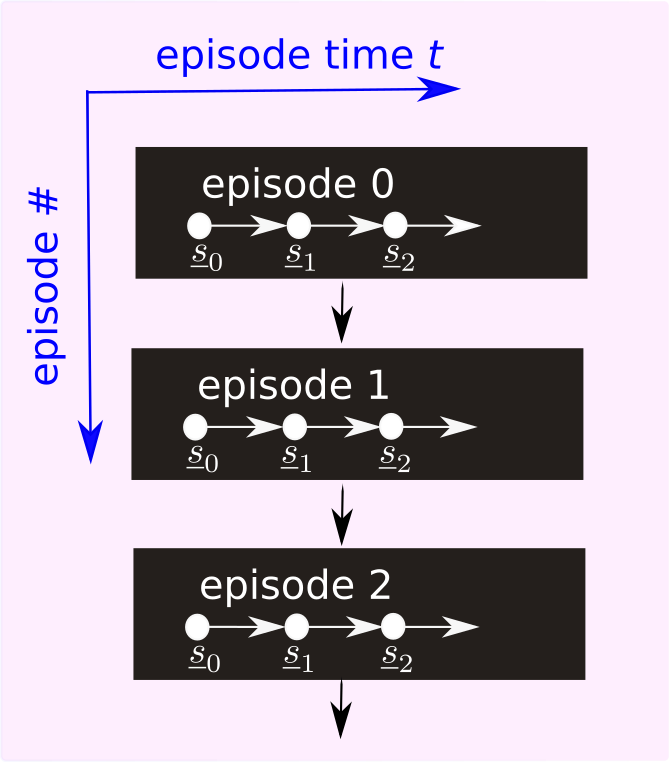
\includegraphics[width=3in]{RL/episodes.png}
\caption{Axes 
for episode time and episode number.} 
\label{fig-epi}
\end{figure}

I based this chapter on the following 
references. Refs.\cite{fox}\cite{levine}

In RL, we consider an ``agent" or
robot that
is learning. 

Let $T\in \ZZ_{>0}$ be the duration time
of an {\bf episode} of learning.
If $T=\infty$, we say that the episode
has an infinite time horizon.
A learning episode will 
 evolve
towards the right,
 for times $t=0,1, \ldots, T-1$. 
We will consider multiple learning episodes.
The episode number will
evolve from top to bottom.
This is illustrated in Fig.\ref{fig-epi}.

 Let $\rvs_t\in S_\rvs $ 
for $t\in [0,T-1]_\ZZ$ be random variables that record the {\bf state} of the
agent at various times $t$.

Let $\rva_t\in S_\rva$ for 
$t\in [0,T-1]_\ZZ$ be random variables that record the {\bf action} of the agent at various times $t$.

Let $\rvtheta_t\in S_\rvtheta$ 
for $t\in [0,T-1]_\ZZ$ be
random variables that record the
 {\bf policy parameters} 
at various times $t$.



For $\rvX\in \{\rvs, \rva, \rvtheta\}$, define $\rvX$ followed by a dot to be the vector 
\beq
\rvX. = 
[\rvX_0, \rvX_1, \ldots, \rvX_{T-1}]
\;.
\eeq
Also let
\beq
\rvX_{\geq t} = 
[\rvX_t, \rvX_{t+1}, \ldots, \rvX_{T-1}]
\;.
\eeq

\begin{figure}
\centering
$$\xymatrix{
\rvtheta_0\ar@/^1pc/[dd]&
\rvtheta_1\ar@/^1pc/[dd]&
\rvtheta_2\ar@/^1pc/[dd]&\\
\rvs_0\ar[r]\ar[d]\ar@/^1pc/[dd]&
\rvs_1\ar[r]\ar[d]\ar@/^1pc/[dd]&
\rvs_2\ar[d]\ar@/^1pc/[dd]\\
\rva_0\ar[ur]\ar[d]&
\rva_1\ar[ur]\ar[d]&
\rva_2\ar[d]
\\
\rvr_0&
\rvr_1&
\rvr_2
}$$
\caption{State-Action-Reward dynamical bnet}
\label{fig-basic-rl}
\end{figure}

Fig.\ref{fig-basic-rl} shows
the basic State-Action-Reward bnet
for an agent that is learning.
The TPMs for the
nodes of Fig.\ref{fig-basic-rl} are
given in blue below:

\beq\color{blue}P(a_t|s_t, \theta_t)\text{ = given.}
\eeq
 $P(a_t|s_t, \theta_t)$ is called  a
{\bf policy with parameter $\theta_t$.} 

\beq\color{blue}P(s_{t}|s_{t-1}, a_{t-1})
\text{ = given.}\eeq
$P(s_t|s_{t-1}, a_{t-1})$ is called the
 {\bf TPM of the model}.
$P(s_t|s_{t-1}, a_{t-1})$ reduces to $P(s_0)$ when $t=0$.

\beq\color{blue}
P(r_t|s_t, a_t)=\delta(r_t, r(s_t, a_t)))
\;.\eeq
$r:S_\rvs\times S_\rva\rarrow \RR$ 
is a given
 {\bf one-time reward function}.


Note that 
\beq
P(s., a.|\theta.)=\prod_{t=0}^{T-1}
\{
P(s_t|s_{t-1}, a_{t-1})
P(a_t|s_t, \theta_t)\}
\;.
\eeq
Define the {\bf all times reward} 
$\Sigma$ by

\beq
\Sigma(s., a.) = 
\sum_{t=0}^{T-1}\gamma^t r(s_t, a_t)
\;.
\eeq
Here $0<\gamma<1$. 
$\gamma$, called the {\bf discount rate},
is included to assure 
convergence of $\Sigma$ when
$T\rarrow \infty$. 
If $r(s_t, a_t)< K$ for all $t$, then
$\Sigma< K \frac{1}{1-\gamma}$.

Define the {\bf objective (i.e. goal)
 function}
$E\Sigma(\theta.)$ by

\beq
E\Sigma(\theta.)=
E_{\rvs., \rva.|\theta.}
\Sigma(\rvs., \rva.)=
\sum_{s., a.}
P(s., a.|\theta.)\Sigma(s., a.)
\eeq
The goal of RL  is to
maximize the 
objective function over
its parameters $\theta.$.
The parameters $\theta^*.$ that 
maximize the objective function 
are the optimum strategy:

\beq 
\theta.^* = \argmax_{\theta.}
E\Sigma(\theta.)
\eeq

\hrule
Define a {\bf future reward} for
 times $\geq t$ as:
\beq
\Sigma_{\geq t}((s_{t'},
 a_{t'})_{t'\geq t}) =
 \sum_{t'=t}^{T-1}\gamma^{t'-t} r(s_{t'}, a_{t'})
\eeq

Define the following {\bf expected conditional 
future rewards} (rewards for times 
$\geq t$,
conditioned on certain quantities
having given values):

\beqa
v_t &=& v(s_t, a_t; \theta.)=E_{\rvs., \rva.|s_t,a_t, \theta.}[\Sigma_{\geq t}]\\
V_t &=& V(s_t;\theta.)=E_{\rvs., \rva.|s_t, \theta.}[\Sigma_{\geq t}]=
E_{\rva_t|s_t, \theta.}[v(s_t, \rva_t;\theta.)]
\eeqa

$v$ is usually called $Q$
in the literature. We will
refer to $Q$ as $v$
in order to follow
a convention wherein an
$\rva_t$-average changes a lower case
letter to an upper case one.  

We will sometimes
write $v(s_t, a_t)$
instead of $v(s_t, a_t;\theta.)$.

Since $E\Sigma_{\geq t}$ only depends on
$\theta_{\geq t}$, $v(s_t, a_t;\theta.)=
v(s_t, a_t;\theta_{\geq t})$, and
$V(s_t;\theta.)=
V(s_t;\theta_{\geq t})$.

Note that the objective function 
$E\Sigma$ can be expressed in terms of 
$v_0$ by averaging over its unaveraged
parameters:
\beq
E\Sigma(\theta.)=
E_{\rvs_0,\rva_0|\theta_0}
v(\rvs_0, \rva_0;\theta.)
\eeq

Define
a {\bf one-time reward}
 and an 
{\bf expected conditional one-time  reward} as:
\beqa
r_t &=& r(s_t, a_t)\\
R_t &=& R(s_t;\theta_t)=
E_{\rva_t|s_t, \theta_t}[r(s_t, \rva_t)]\
\;.
\eeqa


\hrule

Note that

\beqa
\Sigma_{\geq t} &=& r_t + \gamma r_{t+1} 
+ \gamma^2 r_{t+2} +\ldots
+ \gamma^{T-1-t} r_{t+(T-1-t)}\\
&=& r_t + \gamma \Sigma_{\geq t+1}
\label{eq-Sigma}
;.
\eeqa

 
If we take
 $E_{\rvs., \rva.|s_t, a_t, \theta.}
[\cdot]$
of both sides of Eq.(\ref{eq-Sigma}), 
we get

\beq
v_t = r_t + \gamma E_{\rvs_{t+1},
 \rva_{t+1}|\theta.} [v_{t+1}]
\;.
\eeq
If we take $E_{\rvs., \rva.|s_t, \theta.}[\cdot]$
of both sides of Eq.(\ref{eq-Sigma}), 
we get

\beq
V_t = R_t + \gamma E_{\rvs_{t+1}|\theta.}
[V_{t+1}]
\;.
\eeq

Note that
\beqa
\Delta r_t&=& r_t -R_t\\
&=& r_t -(V_t - 
\gamma E_{\rvs_{t+1}|\theta.} [V_{t+1}])\\
&=& r_t
+ \gamma E_{\rvs_{t+1}|\theta.} [V_{t+1}]
-V_t
\;.
\eeqa
Define
\beq
\Delta v_t = v_t - V_t
\;. 
\eeq
Note that 
\beq
\Delta v_t = \Delta r_t
\;.
\eeq

Next, we will discuss 3 RL bnets
\begin{itemize}
\item
exact RL bnet 
(exact, assumes policy is known)
\item
Actor-Critic RL bnet (approximate, 
assumes
policy is known)
\item
Q function learning RL bnet (approximate, 
assumes
policy is NOT known)
\end{itemize}



\section{Exact RL bnet}

\begin{figure}
\centering
$$\xymatrix{
\rvtheta.\ar[d]\ar[dr]\ar[drr]\ar[drrr]
\ar@/_2pc/[dddddd]\\
\rvtheta_0\ar@/^1pc/[dd]&
\rvtheta_1\ar@/^1pc/[dd]&
\rvtheta_2\ar@/^1pc/[dd]&
\rvtheta_3&\\
\rvs_0\ar[r]\ar[d]\ar@/^1pc/[dd]&
\rvs_1\ar[r]\ar[d]\ar@/^1pc/[dd]&
\rvs_2\ar[r]\ar[d]\ar@/^1pc/[dd]&
\rvs_3\\
\rva_0\ar[d]\ar[ur]&
\rva_1\ar[d]\ar[ur]&
\rva_2\ar[d]\ar[ur]&
\rva_3\\
\rvr_0\ar[d]&
\rvr_1\ar[d]&
\rvr_2\ar[d]&
\rvr_3\\
\rvv_0(\cdot)\ar[d]&
\rvv_1(\cdot)\ar[l]&
\rvv_2(\cdot)\ar[l]&
\rvv_3(\cdot)\ar[l]\\
\rvtheta'.
}$$
\caption{Exact RL bnet. 
$v_t(\cdot)$ means the  array
$[v_t(s_t,a_t)]_{\forall s_t, a_t}$ 
The
following arrows 
are implicit:
 for all $t$, arrow
from $\rvtheta.\rarrow \rvv_t(\cdot)$.
We did not draw those arrows
so as not to clutter the diagram.}
\label{fig-exact-rl}
\end{figure}
An exact RL bnet is given by
 Fig.\ref{fig-exact-rl}.


Fig.\ref{fig-exact-rl} is the 
same as Fig.\ref{fig-basic-rl} but
 with more nodes added in order to
optimize the policy parameters.
Here are the TPMs, printed
in blue, 
for the nodes not already discussed
in connection to 
Fig.\ref{fig-basic-rl}.

 

\beq \color{blue}
P(\theta_t|\theta.) =
\delta(\theta_t, (\theta.)_t)
\eeq


\beq\color{blue}\forall (s_t, a_t):\;\;
P(v_t(s_t, a_t)|r_t, v_{t+1}(\cdot),\theta.)
=\delta(v_t(s_t,a_t), r_t + 
\gamma E_{\rvs_{t+1},\rva_{t+1}
|\theta.}[ v_{t+1}])
\eeq

\beq \color{blue}
P(\theta.'|\theta., v_0(\cdot))=
\delta(\theta'.,
\theta. + \alpha\partial_{\theta.}
\underbrace{E_{\rvs_0, \rva_0|\theta_0}
v(\rvs_0, \rva_0
;\theta.)}_{E\Sigma(\theta.)})
\eeq
$\alpha>0$ is called the
{\bf learning rate}. This method
of improving $\theta.$ is 
called gradient ascent.

Concerning the
gradient of the
objective function, note that

\beqa
\partial_{\theta_t}E\Sigma(\theta.)&=&
\sum_{s., a.}
\partial_{\theta_t}P(s., a.|\theta.)
\Sigma(s., a.)\\
&=& 
\sum_{s., a.}P(s., a.|\theta.)
\partial_{\theta_t}
\ln P(s., a.|\theta.)\Sigma(s., a.)
\\
&=&
E_{\rvs., \rva.|\theta.}\left\{
\partial_{\theta_t}
\ln P(a_t|s_t, \theta_t)
\Sigma(s., a.)
\right\}
\;.
\eeqa
If we run the
agent $nsam(\vecs_t)$
times and obtain
samples $s_t[i], a_t[i]$ for all $t$ and
for $i=0, 1, \ldots,nsam(\vecs_t)-1$, 
we can express this  gradient as
follows:

\beq
\partial_{\theta_t}E\Sigma(\theta.)
\approx
\frac{1}{nsam(\vecs_t)}
\sum_{i}\sum_{t=0}^{T-1}
\partial_{\theta_t}
\ln P(a_t[i]\cond s_t[i], \theta_t)
r(s_t[i], a_t[i])
\;.
\label{eq-grad-samples}
\eeq

The exact RL bnet 
Fig.\ref{fig-exact-rl} is difficult to
use to calculate the
optimum parameters $\theta^*.$.
The problem 
is that $\rvs_t$
propagates towards the future
and the $\rvv_t(\cdot)$
propagates towards the past,
so we don't have a Markov Chain 
with a chain link for each $t$ (i.e., 
a
dynamical bnet) in the 
episode time direction.
Hence,
people have come up
with approximate RL bnets
that are
doubly dynamical (i.e.,
dynamical along
the episode time and
episode number axes.)
We discuss some of those
approximate RL bnets next. 



\section{Actor-Critic RL bnet}

For the actor-critic RL 
bnet, 
we approximate Eq.(\ref{eq-grad-samples})
by

\beq
\partial_{\theta_t}E\Sigma(\theta.)
\approx
\frac{1}{nsam(\vecs)}
\sum_{i}\sum_{t=0}^{T-1}
\underbrace{
\partial_{\theta_t}
\ln P(a_t[i]\cond s_t[i], \theta_t)
}_{Actor}
\underbrace{
\Delta r_t(s_t[i], a_t[i])
}_{Critic}
\eeq


\begin{figure}
\centering
$$\xymatrix{
\rvtheta_0\ar@/^1pc/[dd]\ar@/_1pc/[ddddd]&
\rvtheta_1\ar@/^1pc/[dd]\ar@/_1pc/[ddddd]&
\rvtheta_2\ar@/^1pc/[dd]\ar@/_1pc/[ddddd]&
\rvtheta_3\\
\vec{\rvs}_0\ar[r]\ar[d]\ar@/^1pc/[dd]
\ar@/^2pc/[ddd]&
\vec{\rvs}_1\ar[r]\ar[d]\ar@/^1pc/[dd]
\ar@/^2pc/[ddd]\ar[dddl]&
\vec{\rvs}_2\ar[r]\ar[d]\ar@/^1pc/[dd]
\ar@/^2pc/[ddd]\ar[dddl]&
\vec{\rvs}_3\ar[dddl]\\
\vec{\rva}_0\ar[d]\ar[ur]\ar@/^1pc/[dd]&
\vec{\rva}_1\ar[d]\ar[ur]\ar@/^1pc/[dd]&
\vec{\rva}_2\ar[d]\ar[ur]\ar@/^1pc/[dd]&
\vec{\rva}_3\\
\vec{\rvr}_0&
\vec{\rvr}_1&
\vec{\rvr}_2&
\vec{\rvr}_3\\
\ul{\Delta \vec{v}}_0\ar[d]&
\ul{\Delta \vec{v}}_1\ar[d]&
\ul{\Delta \vec{v}}_2\ar[d]&
\ul{\Delta \vec{v}}_3\\
\rvtheta'_0&
\rvtheta'_1&
\rvtheta'_2&
\rvtheta'_3
}$$
\caption{Actor-Critic RL bnet.  }
\label{fig-ac-rl}
\end{figure}
The actor-critic RL bnet
is given by Fig.\ref{fig-ac-rl}. This
bnet is approximate and assumes
that the policy is known. The
TPMs for its nodes
are given in blue below.



\beq\color{blue}
P(\theta_t) \text{ = given}
\eeq

\beq\color{blue}
P(s_t[i]\cond s_{t-1}[i], a_{t-1}[i]) = \text{ given} 
\eeq

\beq\color{blue}
P(a_t[i]\cond s_t[i], \theta_t)= \text{ given}
\eeq

\beq\color{blue}
P(r_t[i]\cond s_t[i],a_t[i])=
\delta(r_t[i],r(s_t[i], a_t[i]))
\eeq
$r:S_\rvs\times S_\rva\rarrow\RR $ is given.

\beq\color{blue}
P(\Delta v_t[i]\cond s_t[i], a_t[i], s_{t+1}[i])=
\delta(\Delta v_t[i], r(s_t[i], a_t[i]) +
\gamma \hat{V}(s_{t+1}[i];\phi')
- \hat{V}(s_t[i]);\phi)
\;.
\eeq

\beq\color{blue}
P(\theta'.)=\delta(\theta'.,
\theta_t +
\alpha \partial_{\theta_t}\sum_i
\ln P(a_t[i]\cond s_t[i], \theta_t )
\Delta v_t[i])
\eeq

$\hat{V}(s_t[i]);\phi)$ is
obtained by curve fitting
 (see Chapter \ref{ch-basic-fit})
using samples $(s_t[i], a_t[i])$ 
$\forall t,i$
with

\beq
 y[i]=\sum_{t'=t}^{T}
r(s_{t'}[i],a_{t'}[i])
\label{eq-V-approx}
\eeq
and 

\beq
\hat{y}[i]=
\hat{V}(s_t[i];\phi)
\;.
\eeq
Eq.(\ref{eq-V-approx}) 
is an approximation
because $(s_{t'}, a_{t'})_{t'>t}$ 
are averaged over in the exact
expression for $V(s_t)$.
$\hat{V}(s_{t+1}[i]);\phi')$ is
obtained in the same way as
$\hat{V}(s_t[i]);\phi)$
but with $t$ replaced by $t+1$
and $\phi$ by $\phi'$.

\section{Q function learning RL bnet}

\begin{figure}
\centering
$$\xymatrix{
\rvs_0\ar[r]\ar[d]
\ar@/^1pc/[dd]&
\rvs_1\ar[r]\ar[d]
\ar@/^1pc/[dd]&
\rvs_2\ar[r]\ar[d]
\ar@/^1pc/[dd]&
\rvs_3\\
\rva_0\ar[d]\ar[ur]&
\rva_1\ar[d]\ar[ur]&
\rva_2\ar[d]\ar[ur]&
\rva_3\\
\rvr_0&
\rvr_1&
\rvr_2&
\rvr_3\\
\rvQ_0(\cdot)\ar@/_1pc/[uu]\ar[r]&
\rvQ_1(\cdot)\ar@/_1pc/[uu]\ar[r]&
\rvQ_2(\cdot)\ar@/_1pc/[uu]\ar[r]&
\rvQ_3(\cdot)
}$$
\caption{Q function learning  RL bnet. }
\label{fig-learn-q}
\end{figure}
The Q-function learning RL bnet
is given by Fig.\ref{fig-learn-q}. This
bnet is approximate and assumes
that the policy is NOT known. The
TPMs for its nodes
are given in blue below. (Remember
that $Q=v$).

\beq\color{blue}
P(s_t|s_{t-1}, a_{t-1}) = \text{ given} 
\eeq



\beq\color{blue}
P(a_t|s_t, v_t(\cdot))=
\delta(a_t, \argmax_{a}v_t(s_t, a))
\eeq

\beq\color{blue}
P(r_t|s_t,a_t)=\delta(r_t, r(s_t, a_t))
\eeq
$r:S_\rvs\times S_\rva\rarrow\RR $ is given.

\beqa\color{blue}\forall (s_t, a_t):\;\;
\lefteqn{P(v_t(s_t, a_t)| 
v_{t-1}(\cdot))=}\nonumber
\\
&\color{blue}=&\color{blue}
\delta(v_t(s_t, a_t), 
r(s_{t}, a_{t})+ \gamma \text{max}_{a}
E_{\rvs_{t+1}|s_{t}, a_{t}}
v_{t-1}(\rvs_{t+1}, a))
\label{eq-sprime-av}
\eeqa
This 
value for $v_t(s_t, a_t)$
approximates $v_t = r_t +\gamma 
E_{\rvs_{t+1}, \rva_{t+1}}v_{t+1}$.

Some people 
use the bnet of 
Fig.\ref{fig-learn-q-approx})
instead of Fig.\ref{fig-learn-q}
and replace 
 Eq.(\ref{eq-sprime-av})
by

\beqa\color{blue}\forall (s_t, a_t):\;\;
\lefteqn{P(v_t(s_t, a_t)| s_{t+1},
v_{t-1}(\cdot))=}\nonumber
\\
&\color{blue}=&\color{blue}
\delta(v_t(s_t, a_t), 
r(s_{t}, a_{t})+ \gamma \text{max}_{a}
v_{t-1}(s_{t+1}, a))
\;.
\eeqa



\begin{figure}
\centering
$$\xymatrix{
\rvs_0\ar[r]\ar[d]
\ar@/^1pc/[dd]&
\rvs_1\ar[r]\ar[d]
\ar@/^1pc/[dd]
\ar[lddd]&
\rvs_2\ar[r]\ar[d]
\ar@/^1pc/[dd]
\ar[lddd]&
\rvs_3
\ar[lddd]\\
\rva_0\ar[d]\ar[ur]&
\rva_1\ar[d]\ar[ur]&
\rva_2\ar[d]\ar[ur]&
\rva_3\\
\rvr_0&
\rvr_1&
\rvr_2&
\rvr_3\\
\rvQ_0(\cdot)\ar@/_1pc/[uu]\ar[r]&
\rvQ_1(\cdot)\ar@/_1pc/[uu]\ar[r]&
\rvQ_2(\cdot)\ar@/_1pc/[uu]\ar[r]&
\rvQ_3(\cdot)
}$$
\caption{Q function learning  RL bnet.
Same as Fig.\ref{fig-learn-q}
but with new arrow
passing $s_t$ to $Q_{t-1}$. }
\label{fig-learn-q-approx}
\end{figure}
\chapter{Simpson's Paradox}
This chapter 
is based on Chapter 6 of 
``The Book of Why", Ref.\cite{book-why}.
See also
Ref.\cite{wiki-simpson}
and references therein.


Simpson's paradox is a recurring 
nightmare for all statisticians 
overseeing a clinical trial for 
a medicine. It is possible that
 if they leave out a certain 
"confounding" variable from a study, 
the study's conclusion on whether
 a medicine is effective or not, might be,
 without measuring that confounding variable, 
the opposite of what it would have 
been had that variable been measured.

Simpson's Paradox is greatly clarified
 by Judea Pearl's theory of causality.
 At the end of this chapter, 
we explain how.

Here is a simple example of 
Simpson's Paradox.

An equal 
number of  patients of male and 
female genders
 are given a heart medicine or a placebo 
in a double blind study.
 Some subsequently have a heart 
attack. Let

$ \ul{a}=$ heart attack? No=0, Yes=1

$ \ul{t}=$ took medicine? No=0, Yes=1

$ \ul{g}=$ gender? Female=0, Male=1



\begin{figure}[h!]
\centering
$$\xymatrix{
&\rvg\ar[dl]&\\
\rva&&\ul{\rvt}\ar[ul]\ar[ll]
}$$
\caption{bnet for a simple example of 
Simpson's paradox.
Here node $g$ is 
a chain junction and a mediator.}
\label{fig-simpson-chain}
\end{figure}

\begin{figure}[h!]
\centering
$$\xymatrix{
&\rvg\ar[dl]\ar[dr]&\\
\rva&&\ul{\rvt}\ar[ll]
}$$
\caption{bnet that is probabilistically
but not physically
equivalent to bnet
Fig.\ref{fig-simpson-chain}.
Here node $g$ is 
a fork junction and a confounder.}
\label{fig-simpson-fork}
\end{figure}




This situation can be modeled by 
either
bnet Fig.\ref{fig-simpson-chain}.
or bnet
 Fig.\ref{fig-simpson-fork}.
The two bnets are 
probabilistically
equivalent 
(i.e., they
both represent the same
probability distribution $P(a, t, g)$)
because

\beq
P(g|t)P(t)=P(g,t)=P(t|g)P(g)
\;.
\eeq

For the bnet
Fig.\ref{fig-simpson-chain}, 
one has

\beq
P(a,g,t)=P(a|g,t)P(g|t)P(t)
\;.
\eeq
Therefore,

\beq
P(a=1|t)=
\sum_g P(a=1|t, g)P(g|t)=E_{\ul{g}|t}
P(a=1|t, \ul{g})
\;,
\eeq
where $ E_{\ul{g}|t}$ is 
a conditional expected value
 (a kind of weighted average).

Suppose $ q_0, q_1$ are 
non-negative real numbers. 
For the vector $ \vec{q}=(q_0, q_1)$:

Define a positive outcome 
(or success or $ q_t$ 
increasing with $ t$) 
if $ q_0 \leq q_1$.

Define a negative outcome 
(or failure or $ q_t$ 
decreasing with $ t$)
 if $ q_0 \geq q_1$.

Let

\beq
\vec{q}^{\;g}=
[P(\rva=1|t,g)]_{t=0,1}
\;
\eeq
for $g=0,1$, and

\beq
\vec{q}^{\;*}=[P(\rva=1|t)]_{t=0,1}
\;.
\eeq

\begin{figure}[h!]
\centering
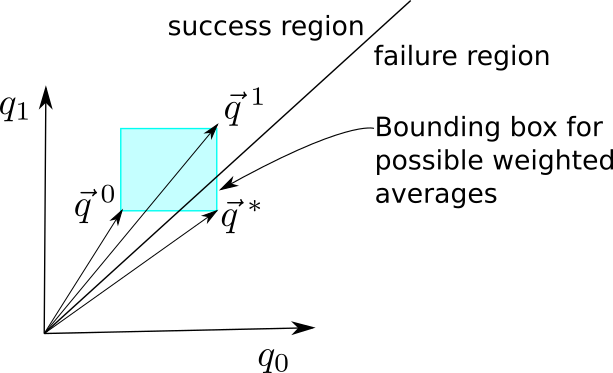
\includegraphics[width=3.5in]
{simpson/q-vecs.png}
\caption{$\vec{q}^{\;0}$,
$\vec{q}^{\;1}$ vectors
and bounding box for vector $\vec{q}^{\;*}$.  } 
\label{fig-simpson-q-vecs}
\end{figure}

It is possible (see Fig.\ref{fig-simpson-q-vecs} 
for a graphical explanation of how)
 to find perverse cases in which
 $ P(a=1|t, g=0)$ and $ P(a=1|t, g=1)$
 increase with $ t$ but $ P(a=1|t)$ 
decreases with $ t$. So it is possible 
to conclude that the medicine is a failure
 for each of the two $ g$ populations 
considered separately, yet the medicine 
is a success when both populations are 
``amalgamated". The lesson is that a
 ``trend reversal" is possible 
upon amalgamation. Trends
are not necessarily preserved 
when we do a weighted average of
 type $ E_{\ul{g}|t}$. 
$ E_{\ul{g}|t}$ is an expected value
 on the random variable $ \ul{g}$
 conditioned on the root 
random variable $ \ul{t}$.


So far, we have proven that probabilistically, 
the drug can be a failure for the populations
 of both sexes considered separately, 
but a success for the aggregate population.

\section*{Pearl Causality}

Pearl Causality would add 
the following two 
important insights 
to this problem:
\begin{enumerate}
\item bnets Fig.\ref{fig-simpson-chain} 
and Fig.\ref{fig-simpson-fork}, 
although they are
probabilistically equivalent, 
do not represent the same physical
 situation. In fact, only
 Fig.\ref{fig-simpson-fork} 
occurs in this case.
\item To decide whether the
 medicine is effective, we 
must apply a $do()$ operator to
 the $ t$ variable in
 Fig.\ref{fig-simpson-fork}. 
The effect of that $do()$ operator
 is to erase the arrow going 
from $ g$ to $ t$. This in turn means
 that the average $ E_{\ul{g}|t}$
 in our equation for $ P(a=1|t)$
 becomes a simpler average $ E_{\ul{g}}$
 which is independent of $ t$. 
But for such an average,
 the
 bounding box in Fig.\ref{fig-simpson-q-vecs}
 degenerates to its diagonal 
line that connects the tips
 of the two vectors $ \vec{q}^{\;0}$
 and $ \vec{q}^{\;1}$. The vector 
$ \vec{q}^{\;*}$ must now fall on 
that diagonal line and must therefore
 also fall in the success region.
\end{enumerate}
In conclusion, as Judea Pearl would say,
 if we ask the right question to Nature,
 i.e., what is
 $ P[a=1 | do(\ul{t}=t)]$ for $ t=0,1$,
 we get as an answer that the 
aggregate population preserves 
rather than reverses the
 unanimous trend of the 
two gendered populations.
\newpage
\section*{Numerical Example}

\begin{table}[h!]
\centering
\begin{tabular}{|l|l|l|}
\hline
\rowcolor[HTML]{ECF4FF} 
(a,t,g) & \begin{tabular}[c]{@{}l@{}}number of patients\\ separated by gender\end{tabular} & \begin{tabular}[c]{@{}l@{}}number of patients\\ of either gender\end{tabular} \\ \hline
0,0,0 & 19 & 47 \\ \cline{1-2}
0,0,1 & 28 &  \\ \hline
0,1,0 & 37 & 49 \\ \cline{1-2}
0,1,1 & 12 &  \\ \hline
1,0,0 & 1 & 13 \\ \cline{1-2}
1,0,1 & 12 &  \\ \hline
1,1,0 & 3 & 11 \\ \cline{1-2}
1,1,1 & 8 &  \\ \hline
\end{tabular}
\caption{Data for numerical example 
 of Simpson's Paradox. This 
fictitious data was taken directly
 from Table 6.4, page 210
of ``The Book of Why", 
Ref.\cite{book-why}.}
\label{tab-simpson-heat-attack}
\end{table}

\beq
P(a|t,g)=
\begin{array}{c|cccc}
&\scriptstyle 0,0 & \scriptstyle 0,1 &
\scriptstyle  1,0 &\scriptstyle 1,1\\\hline
\scriptstyle  0& 19/20 & 28/40 & 37/40 & 12/20\\
\scriptstyle 1& 1/20 & 12/40 & 3/40 & 8/20
\end{array}
\eeq

\beq
P(a|t)=
\begin{array}{c|cc}
&\scriptstyle 0 & \scriptstyle 1\\\hline
\scriptstyle 0& 47/60& 49/60\\
\scriptstyle  1& 13/60 & 11/60
\end{array}
\eeq

\beq
\begin{array}{lll}
\frac{
P(a=1,t=1, g=0)
}{
\sum_aP(a, t=1, g=0)
}=
P(a=1|t=1, g=0) &=& \frac{3}{40}
\\
\frac{
P(a=1,t=0, g=0)
}{
\sum_aP(a, t=0, g=0)
}=
P(a=1|t=0, g=0) &=& \frac{1}{20}=\frac{2}{40}
\end{array}
\label{eq-g-eq-0}
\eeq

\beq
\begin{array}{lll}
\frac{
P(a=1,t=1, g=1)
}{
\sum_aP(a, t=1, g=1)
}=
P(a=1|t=1, g=1) &=& \frac{8}{20}=\frac{16}{40}
\\
\frac{
P(a=1,t=0, g=1)
}{
\sum_aP(a, t=0, g=1)
}=
P(a=1|t=0, g=1) &=& \frac{12}{40}
\end{array}
\label{eq-g-eq-1}
\eeq

\beq
\begin{array}{lll}
\frac{
\sum_g P(a=1,t=1, g)
}{
\sum_g\sum_aP(a, t=1, g)
}=
P(a=1|t=1) &=& \frac{11}{60}
\\
\frac{
\sum_g P(a=1,t=0, g)
}{
\sum_g\sum_aP(a, t=0, g)
}=
P(a=1|t=0) &=& \frac{13}{60}
\end{array}
\label{eq-g-eq-all}
\eeq

Note
that the right hand
side
of 
Eq.\ref{eq-g-eq-0}
is higher
for $t=1$
than for $t=0$.
Same trend 
occurs
in Eqs.\ref{eq-g-eq-1}
but
is reversed in Eqs.\ref{eq-g-eq-all}.
\bibliographystyle{unsrt}
\bibliography{references}
\end{document}	